\documentclass[a4paper, 12pt]{report}
\usepackage{cmap}
\usepackage{amssymb}
\usepackage{amsmath}
\usepackage{graphicx}
\usepackage{amsthm}
\usepackage{upgreek}
\usepackage{setspace}
\setcounter{secnumdepth}{5}
\setcounter{tocdepth}{5}
\usepackage[T2A]{fontenc}
\usepackage[utf8]{inputenc}
\usepackage[normalem]{ulem}
\usepackage{mathtext} % русские буквы в формулах
\usepackage[left=2cm,right=2cm, top=2cm,bottom=2cm,bindingoffset=0cm]{geometry}
\usepackage[english,russian]{babel}
\usepackage[unicode]{hyperref}
\newenvironment{Proof} % имя окружения
{\par\noindent{$\blacklozenge$}} % команды для \begin
{\hfill$\scriptstyle\boxtimes$}
\newcommand{\Rm}{\mathbb{R}}
\newcommand{\Cm}{\mathbb{C}}
\newcommand{\Z}{\mathbb{Z}}
\newcommand{\I}{\mathbb{I}}
\newcommand{\N}{\mathbb{N}}
\newcommand{\rank}{\operatorname{rank}}
\newcommand{\Ra}{\Rightarrow}
\newcommand{\ra}{\rightarrow}
\newcommand{\FI}{\Phi}
\newcommand{\Sp}{\text{Sp}}
\renewcommand{\leq}{\leqslant}
\renewcommand{\geq}{\geqslant}
\renewcommand{\alpha}{\upalpha}
\renewcommand{\beta}{\upbeta}
\renewcommand{\gamma}{\upgamma}
\renewcommand{\delta}{\updelta}
\renewcommand{\varphi}{\upvarphi}
\renewcommand{\phi}{\upvarphi}
\renewcommand{\tau}{\uptau}
\renewcommand{\theta}{\uptheta}
\renewcommand{\eta}{\upeta}
\renewcommand{\lambda}{\uplambda}
\renewcommand{\psi}{\uppsi}
\renewcommand{\mu}{\upmu}
\renewcommand{\omega}{\upomega}
\renewcommand{\d}{\partial}
\renewcommand{\xi}{\upxi}
\renewcommand{\epsilon}{\upvarepsilon}
\renewcommand{\Re}{\operatorname{Re}}
\newcommand{\intx}{\int\limits_{x_0}^x}
\newcommand\Norm[1]{\left\| #1 \right\|}
\newcommand{\sumk}{\sum\limits_{k=0}^\infty}
\newcommand{\sumi}{\sum\limits_{i=0}^\infty}
\newtheorem*{theorem}{Теорема}
\newtheorem*{cor}{Следствие}
\newtheorem*{lem}{Лемма}
\title{\textbf{\Huge{Численные методы}}\\Конспект по 3 курсу 
	специальности «прикладная математика»\\(лектор А. М. Будник)}
\date{}
\begin{document}
	\maketitle
	\tableofcontents{}
	\newpage
	\chapter{Методы решения нелинейных уравнений.}
	В данной главе будут рассмотрены некоторые методы решения нелинейных уравнений и систем уравнений. Рассмотрим случай одного нелинейного уравнения.
	\section{Постановка задачи.}
	Пусть задана функция $f(x)$ действительного переменного $x \in \Rm$. Требуется найти корни уравнения $$f(x) = 0,\eqno(1)$$
	или, что то же самое, нули функции $f(x)$. \\\\
	Выясним, является ли эта задача корректно поставленной. Для ответа на вопрос существования и единственности решения введем теорему из математического анализа.
	\begin{theorem}
		Если функция $f(x)$ непрерывна на отрезке $[a,b]$ и принимает на его концах значения разных знаков, то на этом отрезке существует по крайней мере один корень уравнения $f(x) = 0$.
		Если при этом функция $f(x)$ будет монотонной на отрезке $[a,b]$, то она может иметь только один корень.
	\end{theorem}
	\begin{Proof}
		Без доказательства.
	\end{Proof}\\\\
	Выясним условие устойчивости для рассматриваемой задачи. Как правило, в качестве входных данных мы имеем функцию $f(x)$, заданную в виде функциональной формы. Поэтому понятие устойчивости здесь отпадает.
	\\\\
	Нелинейные уравнения в зависимости от вида функции $f(x)$ можно разделить на два класса:
	\begin{enumerate}
		\item алгебраические;
		\item трансцендентные.
	\end{enumerate}
	В первом классе функция $f(x)$ содержит только алгебраические функции. Например, полином $P_n(x)$ является целой алгебраической функцией. Ко второму же классу относятся все другие функции, которые содержат тригонометрические, показательные, логарифмические выражения и так далее.\\\\
	Методы решения нелинейных уравнений делятся на прямые и итерационные. В курсе численных методов рассматриваются лишь итерационные методы. \\\\
	Задача нахождения корней уравнения (1) обычно решается в два этапа:
	\begin{enumerate}
		\item Отделение корней.\\\\
		На этом этапе изучается расположение корней (в общем случае на комплексной плоскости), проводится их разделение, то есть выделяются области, содержащие только один корень. Кроме того изучается вопрос о кратности корней. Находятся некоторые начальные приближения $x^0$ для точного решения.
		\item Построение метода.
		\\\\
		На этом этапе, используя заданное начальное приближение, строится итерационный процесс, позволяющий уточнить значение отыскиваемого корня до некоторой заданной точности $\epsilon$. То есть, зная начальное приближение $x^0$, мы строим последовательность $x^k \xrightarrow[k\to\infty]{\epsilon}x^*$.
	\end{enumerate}
	В заключение этого параграфа запишем несколько соображений, касающихся первого этапа. По отделению корней мы можем выделить несколько способов нахождения начального приближения:
	\begin{itemize}
		\item из физических соображений;
		\item графический способ;
		\item построение таблицы значений функции $f(x)$ на заданной сетке узлов;
		\item метод деления отрезка пополам (метод дихотомии, метод бисекции).
	\end{itemize}
	Метод деления отрезка пополам заключается в том, что мы берем отрезок $[a,b]$ и смотрим, чтобы на этом отрезке функция меняла знак. Затем делим отрезок пополам, берем точку $c : a<c<b$ и в зависимости от того, где меняется знак, переходим к следующему отрезку $[a,c]$ или $[c,b]$ и так далее. В итоге мы придем к тому, что отрезок получится меньше заданного $\epsilon$, то есть мы и получим искомый корень. Число делений отрезка пополам $$N \geq \log_2 \dfrac{b-a}{\epsilon}.$$
	\section{Метод простой итерации решения нелинейного уравнения.}
	Применение метода простой итерации требует предварительного приведения уравнения $f(x) = 0$ к каноническому виду 
	$$x = \varphi(x), \eqno(1)$$ где $\varphi(x)$ --- это заданная функция. Для канонической формы метод простой итерации будет иметь следующий вид: $$x^{k+1} = \varphi(x^k),\ k = 0,1,2,\ldots,\eqno(2)$$
	где $x^k$ --- последовательность, начинающаяся с $x^0$, которая должна сходится к точному решению. Область изменения аргумента $x$ на числовой оси обозначим через $X$, а через $Y$ обозначим область значений функции $y = \varphi(x)$. Тогда функцию $\varphi(x)$ можно рассматривать как оператор, преобразующий $X$ в $Y$, то есть $$\varphi : X \to Y.$$
	Таким образом, нам нужно найти такие точки области $X$, которые при преобразовании оператором $\varphi$ переходят сами в себя, то есть точки остающиеся неподвижными при преобразовании $X$ в $Y$. Значит решения уравнения $(1)$ --- это точки, остающиеся неподвижными при преобразовании $X$ в $Y$. Геометрически это можно изобразить следующим образом $$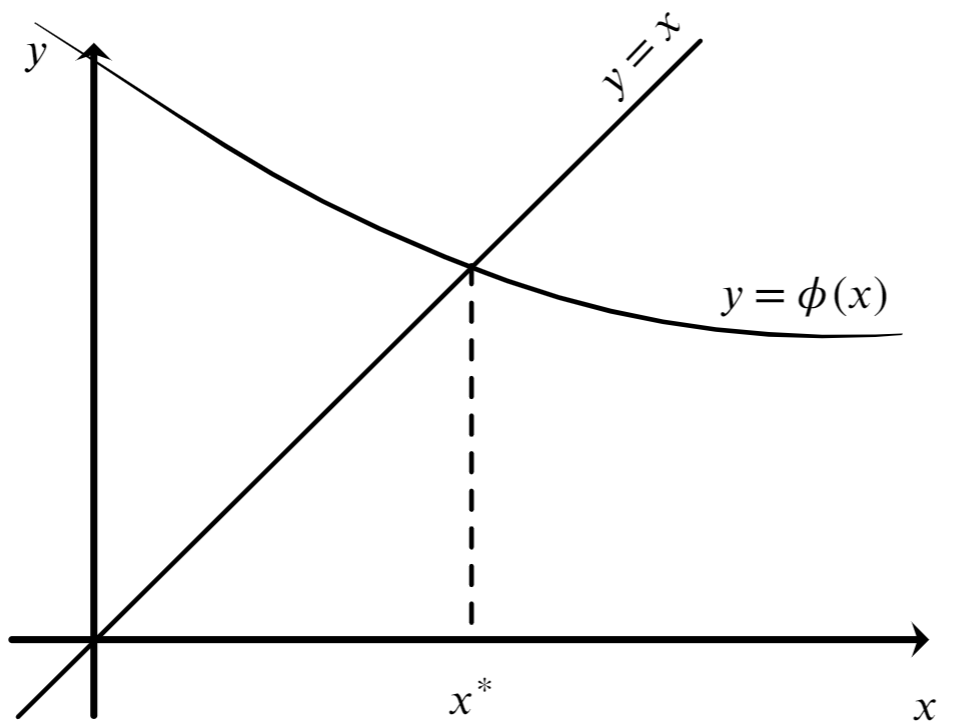
\includegraphics[scale=0.4]{img1.png}$$
	Итак, для решения задачи отыскания корней нелинейного уравнения мы сперва отделяем корни. После процедуры отделения корней мы находим начальное приближение $x^0$ в окрестности корня $x^*$. И по найденному начальному приближению по формуле (2) строится итерационная последовательность, которая и называется \textbf{методом простой итерации.}\\\\
	Мы должны обеспечить сходимость этого итерационного процесса. Сформулируем и докажем для этого теорему.
	\begin{theorem}
		[о сходимости метода простой итерации]
		Пусть выполняются следующие условия:\begin{enumerate}
			\item функция $\varphi(x)$ определена на отрезке $$|x - x^0| \leq \delta,\eqno(3)$$ непрерывна на нем и удовлетворяет условию Липшица с постоянным коэффициентом меньше единицы, то есть $\forall x, \widetilde{x}$ $$|\varphi(x) - \varphi(\widetilde{x})| \leq q |x - \widetilde{x}| ,\quad 0 \leq q < 1;\eqno(4)$$
			\item для начального приближения $x^0$ верно неравенство $$|x^0 - \varphi(x^0)| \leq m;$$
			\item числа $\delta, q, m$ удовлетворяют условию $$\dfrac{m}{1-q}\leq \delta. \eqno(5)$$
		\end{enumerate}
		Тогда \begin{enumerate}
			\item уравнение $(1)$ в области $(3)$ имеет решение;
			\item последовательность $x^k$, построенная по правилу $(2)$, принадлежит отрезку $[x^0 - \delta, x^0 + \delta]$, является сходящейся, и ее предел удовлетворяет уравнению $(1)$: $$x^k \xrightarrow[k\to \infty]{} x^*;$$
			\item скорость сходимости последовательности $x^k$ к ее пределу $x^*$ оценивается неравенством $$|x^* - x^k| \leq \dfrac{m}{1- q}q^k,\ k = 1,2,\ldots \eqno(6)$$
		\end{enumerate}
		Также эта теорема может называется \textbf{методом сжимающих отображений}.
	\end{theorem}
	\begin{Proof}
		Докажем второй пункт, т.е. принадлежность последовательности $x^k$ к отрезку $[x^0 - \delta, x^0 + \delta]$.
		Методом математической индукции покажем, что при всех значениях $k=1,2,\ldots$ приближения $x^k \in [x^0 - \delta, x^0 + \delta]$ и для них верно неравенство $$|x^{k+1} - x^k| \leq mq^k.\eqno(7)$$
		При $k=0$ имеем $x^1 = \varphi(x^0)$, а $x^1$ всегда может быть найден, поскольку $\varphi$ определена в $x^0$. Кроме того  $$|x^1 - x^0| = |\varphi(x^0) - x^0| \leq m,$$ т.е. формула (7) справедлива. Докажем, что $x^1$ находится не дальше чем $m$ от $x^0$: $$m \leq \dfrac{m}{1-q}\leq \delta,$$ отсюда следует, что $x^1 \in [x^0 - \delta, x^0 + \delta]$.
		\\\\
		Пусть данное предположение справедливо при $x^0,x^1,\ldots, x^k \in [x^0 - \delta, x^0 + \delta]$ и $$|x^{n+1} - x^n| \leq mq^n,\ n = 0,1,\ldots, k-1.$$
		По предположению $x^k \in [x^0 - \delta, x^0 + \delta]$. Следовательно, $x^{k+1} = \varphi(x^k)$ может быть вычислено. По сделанному допущению справедливо $$|x^k - x^{k-1}| \leq m q ^{k-1}.$$
		Теперь рассмотрим неравенство для $(k+1)$-ой итерации: $$|x^{k+1} - x^k| = |\varphi(x^k) - \varphi(x^{k-1})|\leq q|x^k - x^{k-1}| \leq mq^k.$$
		Осталось проверить $x^k \in  [x^0 - \delta, x^0 + \delta]$. Рассмотрим разность $$|x^{k+1} - x^0| = \Big|(x^{k+1} - x^k) + (x^k - x^{k-1}) + \ldots + (x^1 - x^0)\Big|\leq mq^k + mq^{k-1} +\ldots + m.$$
		Эта сумма легко подсчитывается как сумма геометрической прогрессии и равна $$\dfrac{m - mq^{k+1}}{1-q} < \dfrac{m}{1-q} \leq \delta.$$
		Итак, мы доказали, что $x^{k+1}$ принадлежит отрезку (3). \\\\
		Докажем сходимость последовательности $x^k$ к решению уравнения $x^*$. Для этого покажем, что для последовательности $x^k$ выполняется условие Больцано-Коши $$|x^{k+p} - x^k| = \Big|(x^{k+p} - x^{k+p-1}) + (x^{k+p-1} - x^{k+p-2}) + \ldots + (x^{k+1} - x^k)\Big|\leq \dfrac{m}{1-q}q^k.$$
		Так как оценка не зависит от $p$, а также учитывая то, что $0\leq q < 1$, можно утверждать, что признак сходимости для последовательности $x^k$ выполняется, а значит существует предел этой последовательности $$\exists \lim\limits_{k\to\infty}x^k = x^*.$$
		Нужно доказать, что $x^* \in [x^0 - \delta; x^0 + \delta]$. Это следует из того, что все $x^k$ принадлежат этому отрезку, то есть и предел находится в этом отрезке. Также нужно доказать, что $x^*$ удовлетворяет уравнению (1). Для доказательства этого в формуле (2) устремим $k\to\infty$, тогда $$x^* = \varphi(x^*).$$
		Ввиду непрерывности функции $x^*$ является решением искомого уравнения, т.е. уравнение (1) превращается в тождество.\\\\
		Последнее, что нужно доказать, --- оценка из третьего пункта теоремы. Для получения неравенства (6) достаточно в соотношении $$|x^{k+p} - x^k| \leq \dfrac{m}{1-q}q^k.$$ устремить $p \to \infty$. Тогда $$|x^* - x^k| \leq \dfrac{m}{1-q}q^k,$$ что и является искомой оценкой.
	\end{Proof}\\\\
	\textbf{Замечания.}\begin{enumerate}
		\item На всяком множестве точек, где для функции $\varphi(x)$ выполняется условие $$|\phi(x) - \phi(y)| <|x-y|,\ x\ne y,$$ уравнение (1) может иметь не более одного решения.
		\item Пользуясь оценкой (6), можно найти априорное количество итераций, необходимое для получения приближенного решения с заданной точностью $$k \geq \dfrac{\lg \frac{\epsilon(1-q)}{m}}{\lg q}.$$
		\item Для построения сходящегося метода простой итерации в практических вычислениях первое условие теоремы о сходимости метода простой итерации обычно заменяется более строгим требованием, а именно для всех $x$ из отрезка $|x - x^0| \leq \delta$ функция $\varphi(x)$ имеет непрерывную первую производную $\varphi'(x)$ такую, что $$|\varphi'(x)|<1 \ \forall x \in [x_0 - \delta; x_0 + \delta].$$
		Более того, если $0\leq\varphi'(x)<1$, то поведение последовательных приближений будет монотонным. Если $-1<\varphi'(x)\leq 0$, то поведение итерационной последовательности будет колебательным.\\\\
		Геометрический смысл метода простой итерации продемонстрируем на графике:
		$$
			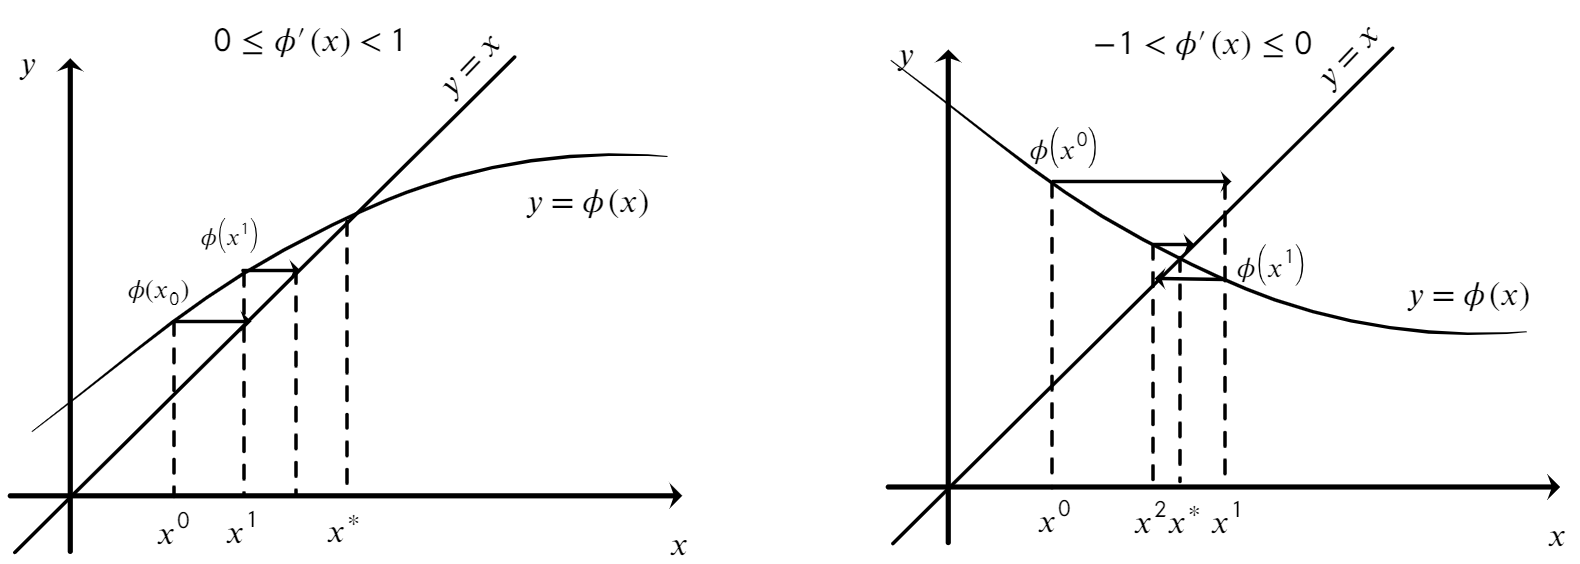
\includegraphics[scale=0.5]{img2}
		$$
		В свою очередь, при $\varphi'(x) > 1$ процесс расходится, это можно увидеть из графика 
		$$
			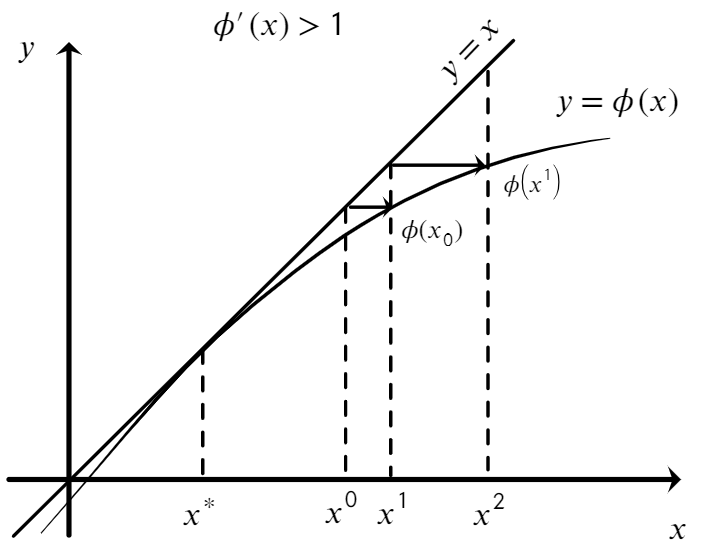
\includegraphics[scale=0.5]{img4}
		$$
		\item Так как сходимость метода простых итераций возможна при сжимающем отображении, то условие $|\varphi'(x)|<1$ является определяющим при приведении исходного уравнения к каноническому виду.
		Наиболее универсальными способом приведения к каноническому виду является преобразование $$x = \underbrace{x+f(x)}_{\varphi(x)},$$
		но нам необходимо выполнение условия $|\varphi'(x)|<1$. Поэтому мы вводим параметр $\psi(x)$, выбираемый таким образом, чтобы обеспечить сходимость: $$x = \underbrace{x+\psi(x)f(x)}_{\varphi(x)},$$ Параметр $\psi(x)$ должен быть непрерывным и  $\psi(x^*)\ne 0.$ Самый простой вариант --- взять постоянную функцию $\psi(x)=\operatorname{const}$ и подобрать эту константу из условия $|\varphi'(x)|<1$.
		\item Поведение последовательности приближений мы будем исследовать, изучая величину $$\epsilon_k = x^* - x^k$$ --- \textbf{погрешность приближенного решения на $k$-ой итерации}. Из этого соотношения легко увидеть, что $$x^k = x^* - \epsilon_k$$ и подставим это в формулу (2). Тогда $$x^* - \epsilon_{k+1} = \varphi(x^* - \epsilon_k).$$
		Предполагая, что функция $\varphi(x)$ имеет непрерывную производную в окрестности точек $x_k$ и $x_{k+1}$, разложим правую часть в ряд Тейлора в окрестности $x^*$:
		$$x^* - \epsilon_{k+1} = \varphi(x^*) - \varphi'(x^*)\epsilon_k + O(\epsilon_k^2).$$ Такое разложение возможно при условии, что функция $\varphi(x)$ дифференцируема и при предположении достаточной малости $\epsilon_k$, чтобы мы могли отбросить остальные члены. Учитывая $x^* = \varphi(x^*)$ и отбрасывая достаточно малые слагаемые $O(\epsilon_k^2)$, получим приближенное равенство $$\epsilon_{k+1} \approx \varphi'(x^*)\epsilon_k.\eqno(8)$$
		Формула (8) дает ответ о скорости сходимости метода простой итерации. То есть погрешность на каждой итерации уменьшается по сравнению с предыдущей в величину $\varphi'(x^*)$. Таким образом, \begin{enumerate}
			\item нам нужно обеспечить $|\varphi'|<1$, чтобы $\epsilon_{k+1} < \epsilon_k$;
			\item сходимость метода осуществляется по закону геометрической прогрессии со знаменателем $q = \varphi'$.
		\end{enumerate}
	\end{enumerate}
	\section{Метод Ньютона решения нелинейного уравнения.}
	Рассмотрим уравнение $$f(x) = 0,\eqno(1)$$ где $f(x)$ достаточно гладкая функция вещественного переменного. Предположим, что для точного решения $x^*$ каким-либо образом задано начальное приближение $x^0$. Для построения метода рассмотрим погрешность $\epsilon_0 = x^* - x^0$. В предположении, что $\epsilon_0$ достаточно малая по модулю величина, подставим в уравнение (1) $x^*$ вместо $x$, тогда $$f(x^0 + \epsilon_0)=0.$$
	Разложим это выражение в ряд Тейлора в окрестности точки $x^0$:$$f(x^0 + \epsilon_0) = f(x^0) + \epsilon_0 f'(x^0) + O(\epsilon_0^2) = 0.$$
	Теперь отбросим слагаемое $O(\epsilon_0^2)$ и получим в рамках отброшенной величины получим приближенное уравнение $$f(x^0) + \epsilon_0 f'(x^0)\approx 0.$$
	Решая это уравнение относительно $\epsilon_0$, получим $$\epsilon_0 \approx -\dfrac{f(x^0)}{f'(x_0)}.$$
	Тогда выразим из $x^* = x^0 + \epsilon_0$ и учитывая, что равенство приближенное, получим $$x^* \approx x^0 - \dfrac{f(x^0)}{f'(x_0)}.$$
	В итоге, повторяя описанную процедуру, мы можем построить итерационную формулу, которая носит название \textbf{метода Ньютона} $$x^{k+1} = x^k - \dfrac{f(x^k)}{f'(x^k)},\quad k = 0,1,\ldots;\quad x_0\eqno(2)$$
	(добавка $x_0$ означает, что начальное приближение задано).
	Иногда этот метод называют \textbf{методом касательных}. Это название следует из геометрического смысла.
	Если рассмотреть уравнение кривой $y = f(x)$, то в точке $x^k$ касательная к ней задается уравнением $$y - f(x^k) = f'(x^k) (x-x^k).$$ Находим точку пересечения касательной с осью $Ox$, полагая $y=0$, и тогда $$x= x^k - \dfrac{f(x^k)}{f'(x^k)}.$$ Таким образом строим приближение $x^{k+1}$ и так далее:
	$$
		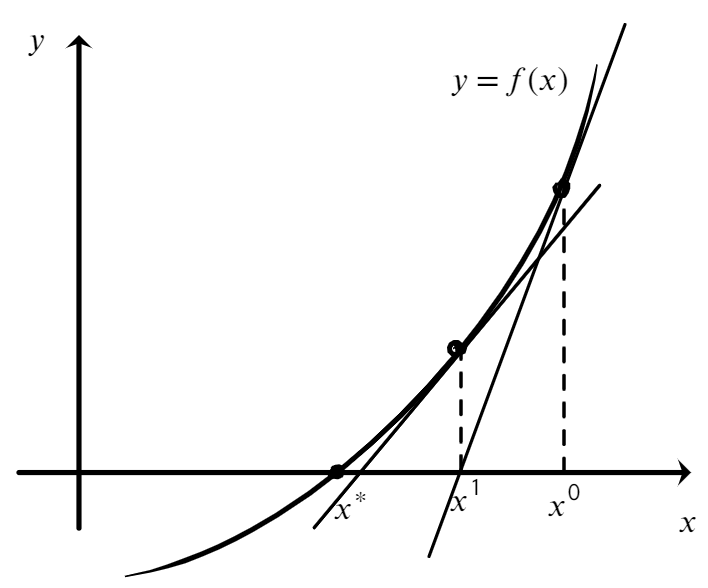
\includegraphics[scale=0.5]{img3}
	$$
	То есть мы приближаемся к корню по последовательности касательных прямых.\\\\
	Выясним, какова скорость сходимости этого метода. С помощью подстановки получим формулу для скорости сходимости $$\epsilon_{k+1} = \dfrac{\epsilon_k f'(x^* - \epsilon_k) + f(x^* - \epsilon_k)}{f'(x^* - \epsilon_k)}.$$ 
	Для того, чтобы получить ответ на вопрос, какова скорость сходимости, необходимо сделать несколько преобразований данного выражения. Воспользуемся тем, что мы можем разложить функции в ряд Тейлора в окрестности $x^*$: $$f(x^* - \epsilon_k) = f(x^*) - \epsilon_kf'(x^*) + \dfrac{1}{2}\epsilon_k^2 f''(x^*) + O(\epsilon_k^3),$$
	$$f'(x^* - \epsilon_k) = f'(x^*) - \epsilon_kf''(x^*) + \dfrac{1}{2}\epsilon_k^2 f'''(x^*) + O(\epsilon_k^3).$$
	В итоге после подстановки мы получим формулу $$\epsilon_{k+1} =- \dfrac{1}{2} \dfrac{f''(x^*)}{f'(x^*)}\epsilon_k^2 + O(\epsilon_k^3).$$
	Отбросив величину более высокого порядка, чем $\epsilon_k^2$, мы получим приближенное равенство $$\epsilon_{k+1} \approx - \dfrac{1}{2} \dfrac{f''(x^*)}{f'(x^*)}\epsilon_k^2=\alpha\epsilon_k^2. \eqno(3)$$
	Формула (3) доказывает, что при $|\alpha|<1$ последовательность $x^k$ построенная по формуле (2) обладает квадратичной сходимостью.
	\begin{theorem}
		[о сходимости метода Ньютона]
		Пусть выполняются следующие условия:
		\begin{enumerate}
			\item Функция $f(x)$ определена и дважды непрерывно дифференцируема на отрезке $$s_0 = [x^0; x^0 + 2h_0],\quad h_0 =- \dfrac{f(x^0)}{f'(x^0)}.$$
			При этом на концах отрезка $f(x)f'(x)\ne 0$.
			\item Для начального приближения $x^0$ выполняется неравенство $$2|h_0|M \leq |f'(x_0)|,\quad M = \underset{x\in s_0}{\max}|f''(x)|.$$
		\end{enumerate}
		Тогда справедливы следующие утверждения: \begin{enumerate}
			\item Внутри отрезка $s_0$ уравнение $f(x) = 0$ имеет корень $x^*$ и при этом этот корень единственный.
			\item Последовательность приближений $x^k$, $k=1,2,\ldots$ может быть построена по формуле $(2)$ с заданным приближением $x^0$.
			\item Последовательность $x^k$ сходится к корню $x^*$, то есть $x^k \xrightarrow[k\to\infty]{}x^*$.
			\item Скорость сходимости характеризуется неравенством $$|x^* - x^{k+1}|\leq |x^{k+1} - x^k|\leq \dfrac{M}{2|f'(x^*)|}\cdot (x^k-x^{k-1})^2,\quad k=0,1,2,\ldots\eqno(4)$$
		\end{enumerate}
	\end{theorem}
	\begin{Proof}
		Сначала докажем утверждение 2, т.е., что последовательность приближений $x^k$ может быть построена. Будем доказывать по индукции. По условию 1 теоремы первый член последовательности (2) можно построить $$x^1 = x^0 - \dfrac{f(x_0)}{f'(x_0)},\quad f'(x_0) \ne 0.$$
		Чтобы доказать возможность построения $x^2$, докажем, что $x^1 \in s_0$ и $f'(x^1)\ne 0$. Учитывая тот факт, что $$x_1  = x_0 + h_0,$$
		получим тот факт, что $x^1$ является серединой отрезка $s_0$. Далее рассмотрим следующее выражение, пользуясь вторым условием, теоремы $$|f'(x^1) - f'(x^0)| = \Big|\int\limits_{x^0}^{x^1} f''(x_0)dx\Big|\leq M|x^1 - x^0| = M | h_0|\leq \dfrac{|f'(x^0)|}{2}.$$
		Теперь рассмотрим $$|f'(x^1)| = \big|f'(x^0) - (f'(x^0) - f'(x^1))\big|\geq |f'(x_0)| - |f'(x^0) - f'(x^1)|\geq |f'(x^0)| - \dfrac{|f'(x^0)|}{2} = \dfrac{|f'(x_0)|}{2} \ne 0.$$
		Таким образом, $f'(x^1)\ne 0$, а значит $x^2$ может быть построено. Тогда $$x^2 = x^1 + h_1,\quad h_1 = -\dfrac{f(x^1)}{f'(x^1)}.$$
		И так далее все $x^k$ могут быть вычислены.\\\\
		 Рассмотрим, как себя ведут отрезки для того, чтобы доказать сходимость итерационного процесса. Наряду с отрезком $s_0$ рассмотрим отрезок $$s_1 = [x^1; x^1 + 2h_1].$$
		Середина этого отрезка --- это $x^2$. Покажем, что $s_1 \subset s_0$. Для этого нам нужно показать, что $h_1 < h_0$. Оценим величину $h_1$. Для этого используем разложение в ряд Тейлора: $$|f(x^1)| = \Big|f(x^0) + h_0f'(x^0) + \dfrac{h_0^2}{2}f''(x^0 + \theta h_0)\Big| = \Big|\dfrac{h_0^2}{2}f''(x^0 + \theta h_0)\Big|\leq \dfrac{h_0^2}{2}M.$$
		$$|h_1| = \Big|-\dfrac{f(x^1)}{f'(x^1)}\Big|\leq \dfrac{h_0^2}{2}\dfrac{M}{|f'(x^1)|}\leq \dfrac{h_0^2}{2}\dfrac{2M}{|f'(x^0)|} = h_0\dfrac{M}{|f'(x^0)|}\leq \dfrac{|h_0|}{2}.$$
		Итак $2|h_1| \leq |h_0|$, следовательно, $$x^1 + 2h_1 = x^0 + h_0 + 2h_1 \leq x^0 + 2h_0 \in s_0.$$
		Отсюда следует, что $s_1 \subset s_0$.\\\\
		Далее мы можем показать по индуктивному предположению, что на отрезке $s_1$ итерация $x^1$ будет удовлетворять условиям 1 и 2 теоремы. Обе части неравенства $|h_1|\leq \dfrac{|h_0|}{2}$ домножим на $\dfrac{2M}{|f'(x^1)|}$, тогда $$\dfrac{2M}{|f'(x^1)|}|h_1|\leq \dfrac{2|h_0| M}{2|f'(x^1)|}$$
		Воспользуемся ранее произведенными оценками:
		$$2|h_0| M \leq |f'(x^0)|,\quad 2|f'(x^1)|\geq \dfrac{1}{2}|f'(x^0)|$$
		Тогда $$\dfrac{2|h_0| M}{2|f'(x^1)|} \leq 1\Rightarrow 2|h_1| M \leq |f'(x^1)|.$$
		Таким образом, на отрезке $s_1$ функция $f(x)$ удовлетворяет условиям теоремы 1 и 2. Теперь по индукции очевидна возможность построения последовательности $x^{k+1}$ по формуле (2). При этом $x^{k+1}$ является серединой отрезка $$s_k = [x^k; x^k + 2h_k], \quad h_k = -\dfrac{f(x^k)}{f'(x^k)}.$$
		А отрезок $s_k\subset s_{k-1}$ и не превосходит половины длины $s_{k-1}$. Кроме того, выполняется неравенство, являющегося оценкой половины длины отрезка $$|h_k| \leq \dfrac{h_{k-1}^2M}{2|f'(x^k)|}.$$
		То есть мы доказали утверждение 2.\\\\
		Докажем утверждения 3 и 1. Так как мы построили последовательность вложенных отрезков $$s_k \subset s_{k-1}\subset \ldots \subset s_1 \subset s_0,$$ длины которых с ростом $k$ стремятся к нулю, то, таким образом, эти отрезки стягиваются в точку. А следовательно последовательность $x^{k+1}$, элементы которой являются серединами этих отрезков, также является сходящейся к некоторому значению $x^*$. Отсюда $$x^{k+1}\xrightarrow[k\to\infty]{} x^*,$$
		но существование предела еще не означает, что это нужный нам предел. Покажем, что $x^*$ -- это корень уравнения (1). Для этого в формуле (2) перейдем к пределу при $k\to\infty$: $$x^* = x^* - \dfrac{f(x^*)}{f'(x^*)},$$ но дробь нужно рассмотреть отдельно. Для того, чтобы перейти к пределу в $f(x^k)$, мы должны доказать, что $$\lim\limits_{k\to\infty}f(x^k) = f(\lim\limits_{k\to\infty}x^k),$$
		этот переход возможен в силу непрерывности функции $f$ и в силу того, что $f'(x^k)\ne 0$ $\forall k$. Тогда записанная нами формула будет верна. А из этой формулы можно сделать вывод, что $$f(x^*) =0.$$
		Теперь докажем единственность этого корня $x^*$. Для этого предположим, что $M > 0$ (случай $M = 0$ мы не рассматриваем, иначе функция будет линейной, а в таком случае на первой же итерации мы получим точное решение). По условию теоремы $$f'(x^0) \ne 0,\quad f'(x^0 + 2h_0) \ne 0.$$
		Учитывая этот факт, мы можем утверждать, что $$f'(x) \ne 0,\quad \forall x \in s_0,$$
		действительно докажем это. Для этого рассмотрим любую точку отрезка $x \in s_0$: $$|f'(x) - f'(x^0)|  = \Big|\int\limits_{x^0}^x f''(t)dt\Big|\leq M|x-x^0| < M \cdot 2|h_0|\leq |f'(x^0)|.$$
		Теперь мы можем оценить величину $\forall x \in s_0$ $$|f'(x)| = |f'(x^0) - (f'(x^0) - f'(x))| \geq |f'(x^0)| - |f'(x^0) - f'(x)|>  |f'(x^0)| - |f'(x_0)| = 0.$$
		То есть $f'(x)\ne 0$ в любой точке отрезка $s_0$. Этот факт говорит о том, что $f(x)$ строго монотонна на $s_0$. Следовательно, уравнение (1) имеет не более одного корня.\\\\
		Докажем утверждение 4. По доказанным ранее утверждениям $x^{k+1}$ --- это середина отрезка $s_k$ длиной $2|h_k|$ и $x^* \in s_k$. Тогда можно рассмотреть $$|x^* - x^{k+1}| \leq |h_k|\leq \dfrac{h_{k-1}^k M}{2 |f'(x^1)|},\ k=0,1,\ldots$$
		Отсюда и следует формула (4).
	\end{Proof}\\\\
	\textbf{Замечания.}\begin{enumerate}
		\item Из оценки (4) можно получить априорную оценку количества итераций, необходимых для достижения заданной точности $\epsilon$ (доказать самостоятельно)
		$$ k \geq \log_2 \dfrac{\ln(\alpha \epsilon)}{\ln(\alpha |x^1 - x^0|)},\quad \alpha = \underset{x\in s_0}{\max}\Big|\dfrac{f''(x)}{2f'(x)}\Big|.$$
		\item Если в окрестности корня производная $f'(x)$ сохраняет знак и монотонна, то приближение $x_k$ построенное по формуле (2) сходится с одной стороны.
	\end{enumerate}
	\section{Видоизменения метода Ньютона и метода простой итерации.}
	\subsection{Модификации метода Ньютона.}
	Все видоизменения связаны с тем, что мы хотим упростить формулу метода Ньютона и уменьшить количество арифметических операций, а для этого будем пытаться заменить вычисление производной вычислением другой более простой функции.
	\subsubsection{Метод Ньютона с постоянной производной.}
	Формула этого метода имеет следующий вид $$x^{k+1} = x^k - \dfrac{f(x^k)}{f'(x^0)},\ k=0,1,\ldots,\quad x^0.$$
	Это видоизменение напрямую связано с уменьшением количества арифметических операции, поскольку мы отказываемся от вычисления последовательности $f'(x^k)$. Таким образом, с точки зрения количества операций метод простой итерации и метод Ньютона становятся сравнимы между собой.\\\\ Геометрически это означает, что, выбрав $x^0$, мы движемся по касательной. Найдя $x^1$, мы будем двигаться из точки $x^1$ по той же касательной, т.е. все касательные будут параллельны касательной в точке, которая является начальным приближением к корню.
	$$
		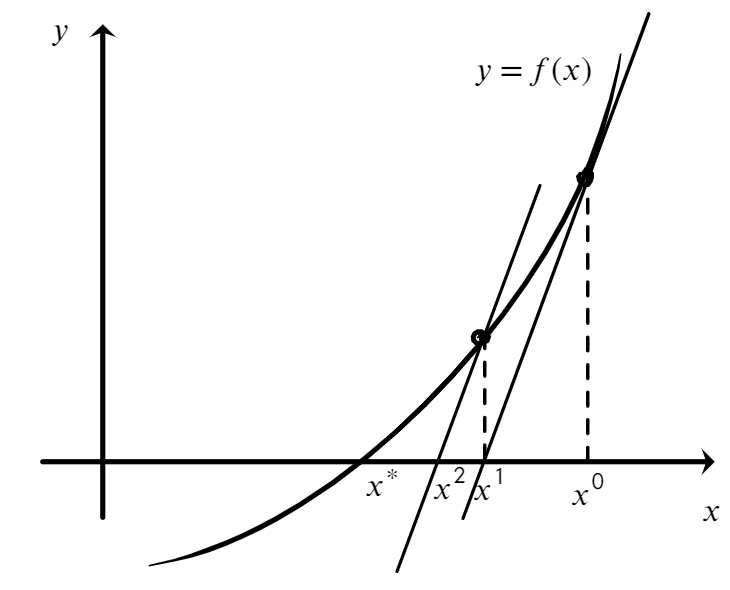
\includegraphics[scale=0.5]{img5}
	$$
	Но скорость сходимости данного метода ухудшится. Легко видеть, что погрешность на каждой итерации будет меняться по следующему закону $$\epsilon_{k+1} = \epsilon_k + \dfrac{f(x^* - \epsilon_k)}{f'(x^0)}.$$
	Проделав необходимые вычисления, связанные с разложением функции в окрестности $x^*$, можно получить $$\epsilon_{k+1}\approx\Big(1 - \dfrac{f'(x^*)}{f'(x^0)}\Big)\epsilon_k.\eqno(2)$$
	Исходя из вида формулы (2), мы можем утверждать, что такая модификация имеет линейную скорость сходимости.
	\subsubsection{Метод секущих.}
	Возьмем за основу формулу производной $$f'(x^k)\approx \dfrac{f(x^k) -f(x^{k-1})}{x^{k} - x^{k-1}},\ k = 1,2,\ldots.$$
	И, подставляя в формулу Ньютона, мы получим следующую формулу $$x^{k+1} = x^k - f(x^k)\dfrac{x^k - x^{k-1}}{f(x^k) - f(x^{k-1})},\ k = 1,2,\ldots;\ x^0,\ x_1\eqno(3)$$
	Однако мы должны знать не только $x^0$, но и $x^1$, поэтому метод секущих двухшаговый.\\\\
	Геометрически мы выбираем два приближения $x^0$ и $x^1$ и через две эти точки мы проводим прямую, и она является не касательной, а секущей. Таким образом, при пересечении секущей с осью $Ox$ мы получаем точку $x^2$. Проводим через $x^1$ и $x^2$ следующую секущую, получаем точку $x^3$ и так далее.
	$$
		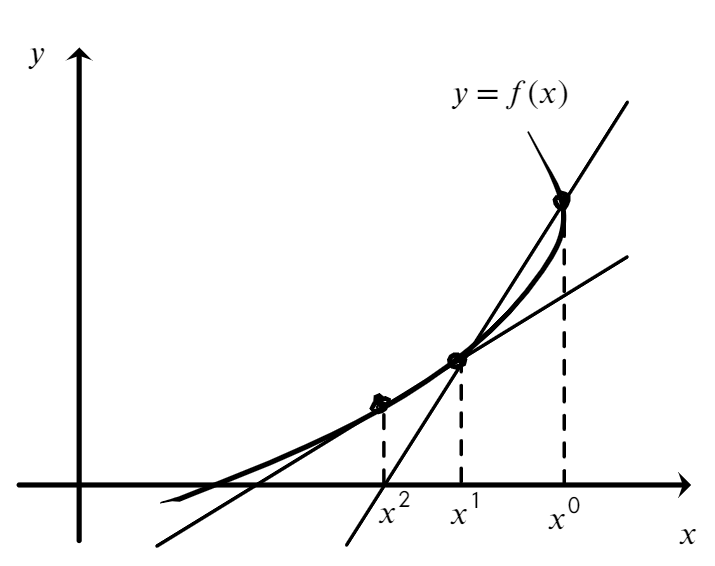
\includegraphics[scale=0.5]{img6}
	$$
Количество операций в этом случае сравнимо с количеством операций метода Ньютона с постоянной производной. Но при этом мы выигрываем в скорости, покажем это. Мы имеем следующее уравнение для погрешности:
$$\epsilon_{k+1} = \epsilon_k - \dfrac{(\epsilon_k - \epsilon_{k+1})f(x^* - \epsilon_k)}{f(x^* - \epsilon_k) - f(x^* - \epsilon_{k-1})}.$$
После выделения главной части из формулы и приведения подобных слагаемых, мы получим соотношение между погрешностями $$\epsilon_{k+1}\approx -\dfrac{1}{2} \dfrac{f''(x^*)}{f'(x^*)}\epsilon_k\epsilon_{k-1}\eqno(4)$$
Таким образом, она выше чем линейная, но ниже, чем квадратичная. Для уточнения необходимо преобразовать данную величину. Соотношение на $k+1$ и $k$ итерациях может быть оценено как $$\epsilon_{k+1}\approx C\epsilon_k^\alpha,\quad \alpha = \dfrac{1+\sqrt5}{2}.$$
\subsubsection{Метод хорд.}
Формула метода хорд имеет вид $$x^{k+1} = x^k - f(x^k)\dfrac{x^k - x^0}{f(x^k) - f(x^0)},\ k=1,2,\ldots;\ x^0, x^1\eqno(5)$$
Для подсчетов нам нужно два приближения, но сам метод одношаговый.\\\\
Геометрически мы строим хорды, проходящие через точку $f(x^0)$ и $f(x^k)$ на каждой итерации. Точка пересечения этой хорды с осью $Ox$ приводит нас к новому приближению $x^{k+1}$:
$$
	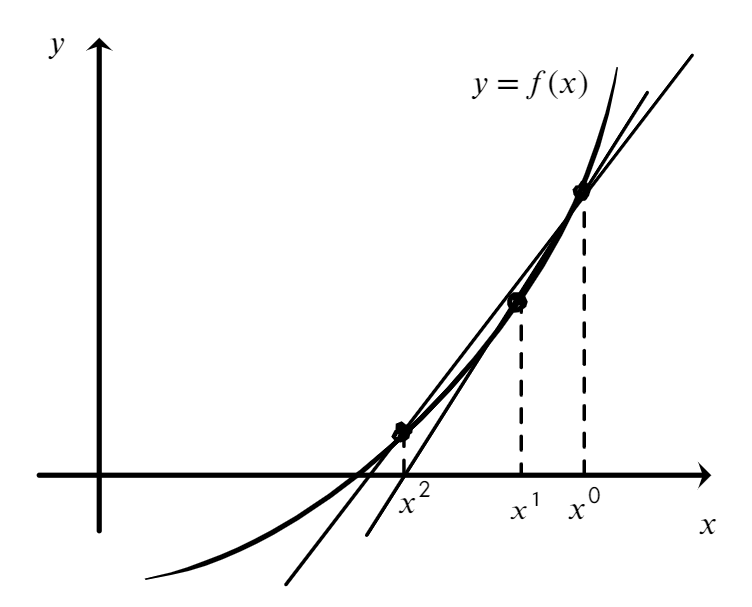
\includegraphics[scale=0.5]{img7}
$$
 В количестве операций мы не выигрываем. Можно показать, что погрешность в данном случае будет иметь вид $$\epsilon_{k+1} \approx -\dfrac{1}{2}\dfrac{f''(x^*)}{f'(x^*)}\epsilon_0\epsilon_k\eqno(6)$$
Отсюда можно сделать вывод, что метод хорд сходится по закону геометрической прогрессии, а значит по линейному закону, но знаменатель прогрессии будет зависеть от $\epsilon_0$. При достаточно хорошем начальном приближении этот метод может сходиться быстрее, чем остальные методы. Практически обычно метод хорд используется для того, чтобы сузить область, где находится корень.
\subsection{Модификации метода простой итерации.}
Все модификации сводятся к тому, что мы хотим повысить скорость сходимости метода.
\subsubsection{Метод Стеффенсена.}
Метод Стеффенсена основывается на том, что мы укажем способ вычисления $x^{k+1}$ через $x^k$ таким образом, чтобы обеспечить квадратичную скорость сходимости. Для увеличения скорости сходимости в данном методе используется преобразование Эйткена. Суть его состоит в том, что, если имеется сходящаяся последовательность чисел $s_0, s_1,\ldots, s_n,\ldots$, которая сходится к числу $s$, и при этом мы знаем, что характер сходимости носит вид $$s_n = s + Aq^n,\quad A = \operatorname{const}, q < 1,$$ то есть сходимость по закону геометрической прогрессии со знаменателем $q$. Тогда закон Эйткена позволяет сразу получить значение искомого предела по формуле Эйткена, построив последовательность $$\sigma_0,\sigma_1,\ldots,\sigma_n, \quad \sigma_n = s = \dfrac{s_{n+1}s_{n-1} - s_n^2}{s_{n+1} - 2s_n + s_{n-1}} = \lim\limits_{n\to\infty} s_n.\eqno(7)$$
Мы будем использовать эту формулу для того, чтобы сразу найти нужный нам предел в методе простой итерации. \\\\
Пусть мы имеем $x^0$. Берем приближения $$x^1 = \varphi(x^0), \quad x^2 = \varphi(x^1) = \varphi(\varphi(x^0)).$$
Тогда, используя формулу (7), мы можем при $n=1$ получить $$\sigma_1 = \dfrac{x^0x^2 - (x^1)^2}{x^2 - 2x^1 +x^0} = \dfrac{x^0 \varphi(\varphi(x^0)) - (\varphi(x^0))^2}{\varphi(\varphi(x^0)) - 2 \varphi(x^0) + x^0}.$$
Заменим в этой формуле соответствующим образом индексы. В итоге получается итерационная формула, которая получила название \textbf{метод Стеффенсена}
$$x^{k+1} = \dfrac{x^k \varphi(\varphi(x^k)) - (\varphi(x^k))^2}{\varphi(\varphi(x^k)) - 2 \varphi(x^k) + x^k},\ k=0,1,\ldots;\ x^0.\eqno(8)$$
Метод Стеффенсена можно трактовать как метод простой итерации примененный к уравнению вида $$x = \Phi(x),$$ где $$\Phi(x) = \dfrac{x \varphi(\varphi(x)) - \varphi^2(x)}{\varphi(\varphi(x)) - 2\varphi(x) + x}.$$ 
Возникает вопрос сходимости метода.
Можно доказать, что функция $\Phi(x)$ вместе со своей производной будет непрерывна в окрестности точки $x^*$, причем $$\lim\limits_{x\to x^*}\Phi(x) = x^*.$$ Если предположить, что функция $\Phi(x^*) = x^*$ (то есть мы доопределяем ее), то $\Phi(x)$ будет непрерывна в точке $x^*$. Кроме того можно утверждать, что $$\Phi'(x^*) = \lim\limits_{x\to x^*}\dfrac{\Phi(x) - \Phi(x^*)}{x - x^*} = 0.$$
Таким образом, можно утверждать, что сходимость метода Стеффенсена будет квадратичной. То есть мы построили метод, обладающий повышенной скоростью сходимости. Но в 2 раза увеличивается объем вычислений, из-за того, что нужно вычислять функцию $\varphi(\varphi(x))$.
\subsubsection{Метод Чебышева.}
Идея метода базируется на способе построения итерационного процесса таким образом, чтобы обеспечить обращение в ноль производных от функции $\varphi(x)$ в точке $x^*$, то есть мы берем уравнение $$x = \varphi(x)$$ и стараемся построить метод, у которого максимальное количество производных обращается в ноль в точке $x^*$. Для этого функцию $\varphi(x)$ запишем в виде $$\varphi(x) = x+ \psi_1(x) f(x) + \psi_2(x)f^2(x) + \ldots + \psi_{n-1}(x)f^{n-1}(x),\eqno(9)$$
где $f(x)$ --- это исходная функция, для которой мы ищем корни. Требуется выбрать функции $\psi_1(x),\ldots, \psi_{n-1}(x)$ так, чтобы $$\varphi^{(j)}(x)\Big|_{f(x)=0} = 0,\quad j=1,2,\ldots,n-1 \eqno(10)$$
Рассмотрим условие на первую производную \begin{multline*}
	\varphi'(x)\Big|_{f(x) = 0} = 1 + \psi_1'(x)f(x) + \psi_1(x) f'(x) + \psi_2'(x) f^2(x) + 2\psi_2(x) f(x) f'(x) + \ldots \Big|_{f(x) = 0}=\\=1 + \psi_1(x) f'(x) \Big|_{f(x) = 0} = 0.
\end{multline*}
Аналогичным образом мы можем записать вторую производную
$$\varphi''(x)\Big|_{f(x) = 0} = 2\psi_1' f'(x) + \psi_1(x) f''(x) + 2\psi_2(x) (f'(x))^2 \Big|_{f(x) = 0} = 0.$$
Из условия $\varphi'(x)\Big|_{f(x) = 0}=0$ следует, что функция $$\psi_1(x) = -\dfrac{1}{f'(x)}.$$ Отсюда $$\varphi(x) = x + \Big(-\dfrac{1}{f'(x)}\Big)f(x),$$ то есть мы пришли к методу Ньютона, итерационному процессу второго порядка.
Из условия, что $\varphi''(x)\Big|_{f(x) = 0}=0$, применяя простые арифметические действия, мы можем получить $$\psi_2(x) = -\dfrac{f''(x)}{2(f'(x))^3}.$$ Учитывая выражения для $\psi_1$ и $\psi_2$ мы можем построить итерационный процесс третьего порядка с кубической скоростью сходимости $$x^{k+1} = x^k - \dfrac{f(x^k)}{f'(x^k)} - \dfrac{f^2(x^k)f''(x^k)}{2(f'(x^k))^3}\eqno(11)$$ и будем называть эту формулу \textbf{методом Чебышева}. В этом методе мы также увеличиваем количество операций, так как необходимо вычислять значения $f(x), f'(x), f''(x)$.
\section{Метод Лобачевского.}
Метод Лобачевского является методом отыскания корней алгебраического уравнения. Данные метод не требует предварительного задания начального приближения для корней и кроме того позволяет найти сразу все корни.\\\\
Рассмотрим алгебраическое уравнение следующего вида $$P(x) = a_0x^n + a_1x^{n-1} + \ldots + a_{n-1}x + a_n = 0,\quad a_0 \ne 0.\eqno(1)$$
Пусть $a_i\in \Rm$ и предположим, что все корни $x_i$ простые, вещественные и удовлетворяют соотношению $$|x_1| >> |x_2| >> \ldots >> |x_n|,\eqno(2)$$ то есть отношение эквивалентно $$\dfrac{|x_{k+1}|}{|x_k|}<<1,\ k=\overline{1,n-1}.$$
Если выполняется условие (2), то говорят, что \textbf{корни сильно разделены} в смысле отношения $(k+1)$-го корня к $k$-ому. \\\\
Из алгебры известно, что соотношение Виета, связывающее корни многочлена с его коэффициентами, является системой вида $$\begin{cases}
	x_1 + x_2 + \ldots + x_n = -\dfrac{a_1}{a_0},\\
	x_1x_2 + x_1x_3 + \ldots + x_{n-1}x_n = \dfrac{a_2}{a_0},\\
	x_1x_2x_3 + \ldots + x_{n-2} x_{n-1}x_n = -\dfrac{a_3}{a_0},\\
	\dotfill\\
	x_1x_2\ldots x_n=(-1)^n\dfrac{a_n}{a_0}.
\end{cases}\eqno(3)$$
В случае выполнения соотношения (2) в левых частях соотношений (3) главными членами будут все первые слагаемые. Тогда вместо точных равенств можно записать приближенные: $$\begin{cases}
x_1 \approx -\dfrac{a_1}{a_0},\\
x_1x_2 \approx \dfrac{a_2}{a_0},\\
x_1x_2x_3 \approx - \dfrac{a_3}{a_0},\\
\dotfill\\
x_1x_2\ldots x_n \approx (-1)^n\dfrac{a_n}{a_0}.
\end{cases}$$
Отсюда можно найти приближенные значения корней
$$x_i \approx -\dfrac{a_i}{a_{i-1}}, i=\overline{1,n}.\eqno(4)$$
Если требование сильной разделенности корней не выполняется, то мы будем строить новое уравнение, корни которого будут высокими степенями корней исходного уравнения. При этом можно надеяться получить уравнение с сильно разделенными корнями. Метод Лобачевского основан на построении уравнения, корни которого являются квадратами корней исходного.\\\\
Запишем уравнение $P(x) =0$ в виде $$P(x) = a_0(x-x_1)(x-x_2)\ldots(x-x_n) =0.$$
Также рассмотрим полином $$P^*(x) = a_0(x+x_1)(x+x_2)\ldots (x+x_n)=0.$$
Корни полинома $P^*(x)$ отличаются от корней исходного уравнения только знаком. По многочленам $P(x)$ и $P^*(x)$ построим многочлен $P_1(y)$ такой, что корнями этого полинома будут являться значения $y_i = x_i^2$, $i=\overline{1,n}.$ Для этого перемножим $$P(x)P^*(x) = a_0^2(x^2 - x_1^2)(x^2 - x_2^2)\ldots(x^2 - x_n^2).$$
Сделав замену $y_i = x_i^2$, мы получим полином $P_1(y)$. Обозначим коэффициенты полинома $P_1(y)$ через $a_i^{(1)}$ и формально перемножим $P(x)$ с $P^*(x)$:
$$P(x)P^*(x) = (a_0x^n + a_{1}x^{n-1} + \ldots + a_n)(a_0x^n - a_1x^{n-1} +\ldots + (-1)^na_n).$$
Тогда коэффициенты нового полинома $$\begin{cases}
	a_0^{(1)} = a_0^2,\\
	a_1^{(1)} =2a_0a_2 - a_1^2,\\
	a_2^{(1)} = 2a_0a_4 - 2a_1a_3 + a_2^2,\\
	\dotfill\\
	a_n^{(1)} = (-1)^na_n^2.
\end{cases}\eqno(5)$$
Предположим, что на основании соотношения (5) мы можем построить последовательность многочленов $$P_k(x) = a_0^{(k)}x^n + a_1^{(k)}x^{n-1} + \ldots + a_n^{(k)}$$ и корнями каждого уравнения $P_k(x) = 0$ будут являться $x_i^{2^k}$, где $x_i$ --- корни исходного уравнения (1). Тогда на каком-то $k$-ом шаге, предполагая сильную разделенность корней, воспользуемся формулой (4) $$x_i^{2^k}\approx - \dfrac{a_i^{(k)}}{a_{i-1}^{(k)}},\quad i =\overline{1,n},$$
а отсюда мы можем извлечь корень степени $2^k$ и найти модули корней исходного уравнения, а их знаки определим подстановкой в многочлен.\\\\
Исследуем вопрос о том, сколько шагов описанного процесса (квадрирования) нужно провести, чтобы получить сильную разреженность корней. Мы укажем один из способов получения условий, который гарантирует сильную разделенность. Пусть процесс квадрирования проведен $k$ раз и мы построили полином $P_k(x)$ такой, что его корни достаточно разделены. Тогда $$\begin{cases}
x_1^{2^k}\approx -\dfrac{a_1^{(k)}}{a_0^{(k)}},\\
x_1^{2^k}x_2^{2^k}\approx \dfrac{a_2^{(k)}}{a_0^{(k)}},\\
\dotfill\\
x_1^{2^k}\ldots x_n^{2^k}\approx (-1)^n\dfrac{a_n^{(k)}}{a_0^{(k)}}.
\end{cases}$$
Теперь мы можем сделать еще один шаг квадрирования 
$$\begin{cases}
	x_1^{2^{k+1}}\approx -\dfrac{a_1^{(k+1)}}{a_0^{(k+1)}},\\
	x_1^{2^{k+1}}x_2^{2^{k+1}}\approx \dfrac{a_2^{(k+1)}}{a_0^{(k+1)}},\\
	\dotfill\\
	x_1^{2^{k+1}}\ldots x_n^{2^{k+1}}\approx (-1)^n\dfrac{a_n^{(k+1)}}{a_0^{(k+1)}}.
\end{cases}$$
Из этих двух систем видно, что $$(x_1^{2^{k+1}}) = (x_1^{2^k})^2.$$
Подставим и получим $$-\dfrac{a_1^{(k+1)}}{a_0^{(k+1)}}\approx \Big(-\dfrac{a_1^{(k)}}{a_0^{(k)}}\Big)^2 \Rightarrow a_1^{(k+1)}\approx -(a_1^{(k)})^2$$
И так далее. При достаточно больших $k$ с требуемой точностью эти величины будут равны. Значит мы достигли требуемой степени разреженности корней. Таким образом, условием того, что достигнута требуемая разделенность корней является следующая связь между коэффициентами многочлена
$$a_i^{(k+1)}\approx (-1)^i(a_i^{(k)})^2.\eqno(6)$$
Тогда, если это выполнено, $x_i$ могут быть посчитаны по формулам $$|x_i| = \sqrt[2^{k+1}]{-\dfrac{a_i^{(k+1)}}{a_{i-1}^{(k+1)}}}\eqno(7)$$
Таким образом, алгоритм метода Лобачевского определен.
\section{Методы решения систем нелинейных уравнений (СНУ).}
В общем виде СНУ можно записать как в координатном виде $$f_i(x_1,\ldots, x_n) = 0,\quad i=\overline{1,n},\eqno(1)$$ так и в векторном виде $$f(x) = 0,\quad f=(f_1,\ldots, f_n)^T,\ x = (x_1,\ldots, x_n)\eqno(1)$$
Частные случаи при $n=1$ -- одно нелинейное уравнение. Если $n>1$, но функции $f_i$ линейные, то получим СЛАУ. Поэтому рассмотрим случай, когда функции нелинейные и $n\geq 2$. Основные этапы решения СНУ:
\begin{enumerate}
	\item отделение корня;
	\item построение последовательности приближений;
	\item контроль сходимости.
\end{enumerate}
Следует иметь ввиду, что проблема отделения корня в общем случае не имеет решений.
\subsection{Метод простой итерации (МПИ).}
Применение метода простой итерации требует приведения исходной системы (1) к виду удобному для итераций, т.е. канонической форме, $$\begin{cases}
	x_1 = \varphi_1(x_1, \ldots, x_n),\\
	\dotfill,\\
	x_n = \varphi_n(x_1,\ldots, x_n);
\end{cases}\eqno(2)$$
или в векторной форме $$x = \varphi(x),\quad \varphi = (\varphi_1,\ldots, \varphi_n)^T,\ x=(x_1, \ldots, x_n).$$
Мы будем предполагать, что $x^*=(x_1^*,\ldots, x_n^*)$ --- точное решение, а $x^k = (x_1^k,\ldots, x_n^k)$ --- итерационное приближение. Если выбрано начальное приближение $x_0$, то все последующие приближения находятся по формуле $$x_{i}^{k+1} = \varphi_i(x_1^k,\ldots, x_n^k), \quad i = \overline{1,n},\ k=0,1,\ldots$$ или в векторной форме $$x^{k+1} = \varphi(x^k)\eqno(3)$$
Будем считать функции $\varphi_i(x)$ непрерывно дифференцируемыми в общей области их задания. Будем далее предполагать, что решение $x^*$ так же, как и все приближения $x^k$, лежат внутри этой области.\\\\
Выясним поведение вектора погрешности $\epsilon^k = (\epsilon_1^k,\ldots, \epsilon_n^k)$ $$\epsilon^k = x^* - x^k = (x_1^* - x_1^k,\ldots, x_n^* - x_n^k)$$
Посмотрим, как будет вести себя погрешность с увеличением количества итераций. Для этого подставим в формулу (3) выражение $x^k$ через $\epsilon^k$ и получим следующее выражение $$x_i^* - \epsilon_i^{k+1} = \varphi_i(x_1^* - \epsilon_1^k,\ldots, x_n^* - \epsilon_n^k).$$
Разложим правую часть последних равенств по степеням $\epsilon^k$ в окрестности точки $x^*$ и выделим главную часть, учитывая, что $x^* = \varphi(x^*)$. Тогда получим $$\epsilon_i^{k+1} = \sum_{j=1}^{n}\dfrac{\partial}{\partial x_j}\varphi_i(x_1^*,\ldots, x_n^*)\epsilon_j^* + O\Big(\max_j (\epsilon_j^k)^2\Big),\quad i = \overline{1,n}.$$
Если мы предположим, что $\epsilon_j^k$ достаточно малые, то можем отбросить достаточно малые слагаемые и записать приближенно отношения между $k$-ой и $(k+1)$-ой итерациями: $$\epsilon^{k+1}\approx A\epsilon^k\eqno(4)$$
где $A$ -- это матрица Якоби построенная по системе функций $\varphi_i$:
$$A = \begin{pmatrix}
	\dfrac{\partial \varphi_1(x^*)}{\partial x_1} & \dots & \dfrac{\partial \varphi_1(x^*)}{\partial x_n}\\
	\vdots & \ddots & \vdots\\
	\dfrac{\partial \varphi_n(x^*)}{\partial x_1} & \dots & \dfrac{\partial \varphi_n(x^*)}{\partial x_n}
\end{pmatrix}$$ 
Таким образом, видно что вектор погрешности на одном шаге испытывает линейное преобразование. Для того, чтобы сделать вывод об условиях сходимости, преобразуем формулу (4). Запишем спектральное разложение матрицы $A$. Предположим, что все элементарные делители матрицы $A$ являются простыми. Тогда эту матрицу можно записать в виде спектрального разложения $$A = S^{-1}\Lambda S,\quad \Lambda = \operatorname{diag}\{\lambda_1,\ldots, \lambda_n\}$$
Тогда соотношение (4) можно записать в виде $$\epsilon^{k+1} \approx S^{-1}\Lambda S \epsilon^k.$$
Обозначим $$r^k = S \epsilon^k.$$
Домножим обе части слева на $S$, тогда $$r^{k+1}\approx \Lambda r^k$$
или покоординатно $$r_i^{k+1} = \lambda_i r^k_i,\quad i=\overline{1,n}$$
Если все $|\lambda_i| <1$ $\forall i$, то $$r_i^k\xrightarrow[k\to \infty]{}0.$$ По условию $\epsilon^k = S^{-1}r^{k}$, а значит $$\epsilon^k\xrightarrow[k\to \infty]{}0.$$
Тогда можно утверждать, что $$x^k\xrightarrow[k\to\infty]{} x^*.$$
Таким образом, необходимым и достаточным условием сходимости является условие $|\lambda_i| <1$ $\forall i$ (по аналогии с МПИ для СЛАУ). Но в практических целях проверка этого условия достаточно затруднительна. Сформулируем теорему о достаточных условиях сходимости МПИ в случае СНУ.
\begin{theorem}
	[о сходимости МПИ в случае СНУ]
	Пусть выполняются условия\begin{enumerate}
		\item функции $\varphi_i(x_1,\ldots, x_n)$ определены и непрерывно дифференцируемы в области $$S_\delta = \max_{1\leq i \leq n}|x_i - x^0_i|\leq \delta;$$
		\item функции $\varphi_i$ удовлетворяют на $S_\delta$ неравенству
		$$\max_{1\leq i \leq n} \max_{x \in S_\delta} \sum_{j=1}^{n}\Big|\dfrac{\partial \varphi_i(x)}{\partial x_j}\Big|\leq q < 1;$$
		\item для начального приближения $x^0$ выполняется условие $$\max_{1\leq i \leq n}|x_i^0 - \varphi_i(x_1^0,\ldots, x_n^0)| \leq m;$$
		\item для чисел $m,\delta, q$ выполняется неравенство $$\dfrac{m}{1-q}\leq \delta.$$
	\end{enumerate}
	Тогда исходная система (2) в области $S_\delta$ имеет решение $x^*$, к которому сходится итерационная последовательность $x^k$, вычисляемая по правилу (3). Кроме того скорость сходимости $x^k \to x^* \in S_\delta$ определяется неравенством $$\max_{1\leq i \leq n}|x_i^* -x_i^k|\leq \dfrac{m}{1-q}q^k.$$
\end{theorem}
\begin{Proof}
	Аналогично подобной теореме для одномерного случая.
\end{Proof}
\subsection{Видоизменения метода простой итерации.}
\subsubsection{Метод Зейделя.}
Аналогично методу Зейделя для СЛАУ, уточненную координату $x_i$ мы будем использовать при уточнении следующей координаты:
$$\begin{cases}
	x_1^{k+1} = \varphi(x_1^k, x_2^k,\ldots, x_n^k),\\
	x_2^{k+1} = \varphi(x_1^{k+1}, x_2^k,\ldots, x_n^k),\\
	\dotfill\\
	x_n^{k+1} = \varphi(x_1^{k+1}, x_2^{k+1},\ldots, x_n^k),
\end{cases} \eqno(5)
$$ или в более компактной форме $$x_i = \varphi_i(x_1^{k+1},\ldots x_{i-1}^{k+1}, x_i^k,\ldots, x_n^k),\quad i=\overline{1,n},\ k=0,1,\ldots\eqno(5)$$
-- \textbf{метод Зейделя} для системы (2). Скорость сходимости метода Зейделя линейная, как и у МПИ. Достаточное условие сходимости аналогично достаточному условию сходимости для МПИ, за исключением того, что в условии 2 теперь $$\Norm{\dfrac{\partial \varphi(x)}{\partial x}}_1 < 1,\quad x \in S_\delta,\quad \Norm{x-x^0}_1\leq \delta.\eqno(6)$$
\subsubsection{Метод Гаусса-Зейделя.}
В отличие от метода Зейделя это видоизменение не требует предварительного приведения приведения системы (1) к каноническому виду. Итерационный процесс будет выглядеть следующим образом $$\begin{cases}
	f_1(x_1^{k+1},x_2^k,\ldots,x_n^k) = 0,\\
	f_2(x_1^{k+1},x_2^{k+1},\ldots,x_n^k) = 0,\\
	\dotfill\\
	f_n(x_1^{k+1},x_2^{k+1},\ldots,x_n^{k+1}) = 0.
\end{cases}\quad k=0,1,\ldots\eqno(7)$$
Нахождение каждого нового значения $x_i^{k+1}$ требует решения нелинейного уравнения вида $$f_i(x_1^{k+1},\ldots, x_{i-1}^{k+1}, x_i^{k+1}, x_{i+1}^k, \ldots, x_n^k) = 0,$$
где все $x_j^k, j>i$ известны как значения с предыдущей итерации, а значения $x_j^{k+1}, j<i$ также известны как координаты точек, которые мы ранее вычислили. Тогда уравнение является уравнением от одной переменной $x_i^{k+1}$. Тогда для решения этого уравнения мы можем применять методы, используемые для одного уравнения.\\\\
Таким образом, мы получаем два вложенных итерационных процесса: внешний и внутренний.\\\\
В качестве примера запишем метод Гаусса-Зейделя с организацией внутреннего итерационного процесса по методу Ньютона (индекс $k$ -- внешний итерационный процесс, а $s$ -- внутренний)
$$x_i^{k+1, s+1} = x_i^{k+1, s} - \dfrac{f_i(x_1^{k+1},\ldots, x_{i-1}^{k+1}, x_i^{k+1, s}, x_{i+1}^k, \ldots, x_n^k)}{\dfrac{\partial}{\partial x_i} f_i(x_1^{k+1},\ldots, x_{i-1}^{k+1}, x_i^{k+1, s}, x_{i+1}^k, \ldots, x_n^k)},\quad s = 0,1,\ldots\eqno(8)$$
В качестве начального приближения возьмем значение соответствующей компоненты, полученное на предыдущей внешней итерации $$x_i^{k+1, 0} = x_i^k.$$
\subsection{Метод Ньютона.}
Построение итерационной последовательности аналогично случаю одного уравнения. Обозначим погрешность $$\epsilon^k = x^* - x^k.$$
Подставим $x^*$ в уравнение и получим $$f(x^k + \epsilon^k) = 0.$$
Разложим в ряд Тейлора левую часть по степеням $\epsilon^k$ в окрестности $x^*$, отбросив достаточно малые слагаемые:
$$f(x^k) + \dfrac{\partial f(x^k)}{\partial x} \epsilon^k\approx 0.$$
Обозначим $$\Delta x^k \approx \epsilon^k,$$ тогда получим следующее выражение $$\dfrac{\partial f(x^k)}{\partial x}\Delta x^k = -f(x^k).\eqno(9)$$
Таким образом, если матрица Якоби $\dfrac{\partial f(x^k)}{\partial x}$ будет невырожденной, то из последнего равенства можно единственным образом найти вектор поправок $\Delta x^k$. Тогда, зная $\Delta x^k$, мы можем построить итерационный процесс $$x^{k+1} = x^k + \Delta x^k.\eqno(10)$$
Если из (9) выразить $\Delta x^k$ и подставить в формулу (10), то можно получить объединенную формулу $$x^{k+1} = x^k - \Big(\dfrac{\partial f(x^k)}{\partial x}\Big)^{-1}f(x^k),\quad k=0,1,\ldots\eqno(11)$$ --- \textbf{метод Ньютона} решения СНУ.\\\\
Если мы будем решать систему линейных алгебраических уравнений (9) итерационными методами, то мы снова получим вложенные итерационные процессы.\\\\
На качественных примерах можно показать, что этот метод будет обладать более высокой скоростью сходимости нежели метод простой итерации.\\\\
Сформулируем теорему о сходимости метода Ньютона для СНУ.
\begin{theorem}
	[о сходимости метода Ньютона для СНУ]
	Пусть в области $$\Omega(x^*, \delta) = \{x\in \Rm: \Norm{x^* - x}\leq \delta\}$$ при некоторых значениях $\delta>0$ и значениях констант $0\leq a_1, a_2<\infty$ выполнены условия \begin{enumerate}
		\item $$\Norm{\Big(\dfrac{\partial f(x^k)}{\partial x}\Big)^{-1}}\leq a_1\quad \forall x \in \Omega(x^*, \delta);$$
		\item $$\Norm{f(x') - f(x'') - \dfrac{\partial f(x'')}{\partial x}(x'-x'')}\leq a_2\Norm{x' -x''}^2,\quad \forall x', x'' \in \Omega(x^*, \delta);$$
		\item $$x^0 \in \Omega(x^*, b),\quad b = \min\{\delta, c^{-1}\},\ c = a_1\cdot a_2.$$
	\end{enumerate}
	Тогда метод Ньютона $(11)$ сходится в области $\Omega(x^*, b)$ и имеет место оценка погрешности $$\Norm{x^k - x^*}\leq \dfrac{1}{c}\Big(c \Norm{x^0 - x^*}\Big)^{2^k}.$$
\end{theorem}
\textbf{Замечания.}\begin{enumerate}
	\item Из оценки погрешности следует квадратичная сходимость метода Ньютона.
	\item В отличие от одномерного случая существования решения  $x^*$ предполагается, что существует обратная матрица $\Big(\dfrac{\partial f}{\partial x}\Big)^{-1}$.
	\item Условие 2 теоремы выполняется автоматически, если функция $f\in C^{2}(\Omega(x^*, \delta))$.
\end{enumerate}
\subsection{Видоизменения метода Ньютона.}
\subsubsection{Метод Ньютона с постоянной матрицей Якоби.}
Запишем формулы метода $$\dfrac{\d f(x^0)}{\d x}\Delta x^k = -f(x^k),\quad x^{k+1} = x^k + \Delta x^k,\ k=0,1,\ldots\eqno(12)$$
Данное видоизменение характеризуется тем, что на каждой итерации необходимо решать СЛАУ с одной и той же матрицей. Это позволяет уменьшить объем вычислений на каждом $k$-ом шаге. 
\subsubsection{Дискретный метод Ньютона.}
Задаем некоторый векторный параметр $h^k \in \Rm^n$, все компоненты которого достаточно малы (близки к нулю) для того, чтобы обеспечить требуемую точность. Тогда частные производные, которые входят в матрицу Якоби, мы приближенно заменяем на разность: $$\dfrac{\d f_i(x_1,\ldots, x_n)}{\d x_j} \approx \dfrac{f_i(x_1,\ldots, x_j,\ldots, x_n) - f_i(x_1,\ldots, x_j-h_j^k,\ldots, x_n)}{h_j^k}.$$
Тогда матрица Якоби в методе Ньютона заменяется некоторой матрицей: $$\begin{pmatrix}
	\dfrac{\d f(x^k)}{\d x}
\end{pmatrix}\sim J(x^k, h^k),$$
элементами которой являются отношения, указанные выше. Тогда получится следующий метод: $$J(x^k, h^k) \Delta x^k =  -f(x^k),\quad x^{k+1} = x^k + \Delta x^k,\ k=0,1,\ldots\eqno(13)$$  --- дискретный метод Ньютона.
\subsubsection{Метод секущих.}
Это частный случай дискретного метода. В данном случае мы будем рассматривать разность $$h^k = x^k - x^{k-1}.$$
Тогда $$\dfrac{\d f_i(x_1^k,\ldots, x_n^k)}{\d x_j}\approx \dfrac{ f_i(x_1^k,\ldots, x_j^k,\ldots, x_n^k) - f_i(x_1^k,\ldots, x_j^{k-1},\ldots, x_n^k)}{x_j^k - x_j^{k-1}}.\eqno(14)$$
Таким образом, с учетом последней формулы мы получим метод вида (13), где элементы матрицы $J(x^k, h^k)$ определяются по формулам (14).
\subsection{Метод градиентного спуска.}
На основании исходной системы нелинейных уравнений системы (1) рассмотрим функцию $$\Phi(x) = \sum\limits_{i=1}^n f^2_i(x_1,\ldots, x_n).\eqno(15)$$
Функция $\Phi(x)$ неотрицательна и обращается в ноль тогда и только тогда, когда все $f_i \equiv 0$. Таким образом, решение исходной системы нелинейных уравнений будет одновременно нулевым минимумом скалярной функции многих переменных $\Phi(x)$.\\\\
По методу градиентного спуска итерационная последовательность к решению определяется формулой $$x^{k+1} = x^k - t\operatorname{grad} \Phi(x^k),\quad k=0,1,\ldots,\ t\geq 0\eqno(16)$$
Параметр $t$ выберем из условия минимума функции $\Phi$ в точке $x^{k+1}$:
$$\Phi(x^{k+1}) = \Phi(x^k - t\operatorname{grad} \Phi(x^k)) = \varphi (t).$$
И будем искать такую функцию, чтобы $\varphi(t)$ была минимальна. \\\\
В итоге, решая уравнение $$\varphi'(t) = 0,$$ находим $t$ на каждой итерации. Таким образом и строится формула (16). Для того, чтобы найти $t$ из этого уравнения, можно использовать любой метод для нахождения корня нелинейной функции одной переменной. \\\\
Иногда функцию $\varphi(t)$ бывает сложно посчитать. Условие $\varphi'(t) = 0$ можно заменить эквивалентным ему. Выразим $$\operatorname{grad} \Phi(x) = 2 (f_i,\operatorname{grad} f_i).$$
И пользуясь выражением для градиента, мы можем записать уравнение $\varphi'(t) = 0$ в следующем виде: $$\sum_{i=1}^{n} 2 f_i (x^k - t\operatorname{grad} \Phi(x^k))\cdot \dfrac{d}{dt}f_i(x^k - t\operatorname{grad} \Phi(x^k)) =0\eqno(17)$$
Для определения $t$ можно использовать один из методов решения нелинейных уравнений.\\\\
\textbf{Замечания}.\begin{enumerate}
	\item Если решить уравнение относительно $t$ не представляется возможным, то требование $\varphi'(t) = 0$ заменяется на менее жесткое: $$\Phi(x^{k+1}) < \Phi(x^k).$$
	\item Методы спуска сходятся для гладких функций всегда, но зачастую довольно медленно. Но они могут использоваться для получения хорошего начального приближения к решению, чтобы использовать более быстро сходящиеся методы.
\end{enumerate}
\chapter{Приближение функций.}
\section{Общие положения проблемы приближения функций.}
В самом широком смысле проблему приближения функций мы сформулируем следующим образом:\begin{enumerate}
	\item имея значения функции $f(x_i)$ в одних точках, найти значения функции в других точках;
	\item имея некоторую функцию $f(x)$, которую трудно вычислить, мы будем заменять ее другой функцией $\varphi(x)$, которую легко вычислить, при этом задача, связанная с приближением функций, состоит в том, чтобы найти такую функцию $\varphi(x)$ и она приближала функцию $f(x)$ с некоторой точностью $\epsilon$.
\end{enumerate}
Примеры задач в рамках поставленной проблемы:
\begin{enumerate}
	\item Задачи планирования экспериментов;
	\item Задачи обработки данных экспериментов;
	\item Задачи вычисления элементарных или специальных функций.
\end{enumerate}
Для решения задачи приближения функции можно рассматривать некоторую функцию $f(x) \in \mathcal F$. Для нее ставится задача -- приблизить или заменить ее другой функцией $\varphi(x,a)\in \Phi (x, a)\subset \mathcal F$, где $a$ -- это некоторый векторный параметр. В зависимости от способа оценки близости $f$ и $\varphi$ получаются различные способы приближения. Укажем два из них:
\begin{itemize}
	\item наилучшее приближение (для решения задачи 1);
	\item интерполяционное приближение (для решения задач 2 и 3).
\end{itemize}
Мы будем рассматривать так называемые линейные задачи приближения функций.
\\\\ 
$\bullet$ \textit{Задача приближения функции называется \textbf{линейной}, если множество $\Phi(x,a)$ размерности $n+1$ линейно относительно параметра $a=(a_0,a_1,\ldots, a_n)$. Таким образом, $\Phi(x,a)$ является линейным подпространством исходного пространства $\mathcal{F}$, натянутым на базисные функции $\varphi_k(x)$, $k=\overline{0,n}$, $x = (x_0,x_1,\ldots, x_n)$. В противном случае задача будет \textbf{нелинейной}.}\\\\ 
В зависимости от аргументов $x_i$ наиболее часто употребляются следующие случаи определения функции $\varphi(x,a)$:
\begin{enumerate}
	\item полиномиальное приближение;
	\item экспоненциальное приближение;
	\item тригонометрическое приближение;
	\item дробно-рациональное приближение.
\end{enumerate}
\section{Наилучшее приближение функции.}
\subsection{Общая постановка задачи.}
Пусть $R$ --- линейное нормированное пространство, $f\in R$ --- элемент, который нужно приблизить. Возьмем в $R$ $(n+1)$ элементов $\varphi_i$, $i=\overline{0,n}$, причем пусть они являются линейно независимыми. С помощью этой системы функций образуем линейное подпространство $\Phi$ всевозможных линейных комбинаций вида $$\varphi = \sum_{i=0}^n c_i\varphi_i,\eqno(1)$$
 где $c_i$ --- действительные коэффициенты. Рассмотрим числовое множество $$\Delta (f,\varphi) = \Norm{f - \varphi}\eqno(2)$$ где $f$ --- фиксированный элемент, а $\varphi$ --- произвольный элемент из $\Phi$. Это числовое множество (2) ограничено снизу, то есть $\exists \Delta (f)$:
 $$\Delta (f) = \underset{\varphi \in \Phi}{\inf} \Delta (f,\varphi)\eqno(3)$$
 $\bullet$ \textit{Величина $\Delta (f)$ называется \textbf{наилучшим приближением элемента} $f$ на множестве $\Phi$.} \\\\
 $\bullet$ \textit{Элемент $\varphi^*\in \Phi$, для которого выполняется равенство (3), называется \textbf{элементом наилучшего приближения} $f$ на $\Phi$.}
 \begin{theorem}
 	Для любого элемента $f \in R$ в подпространстве $\Phi$ существует элемент наилучшего приближения.
 \end{theorem}
 \begin{Proof}
 	Без доказательства.
 \end{Proof}\\\\
 $\bullet$ \textit{Нормированное пространство называется \textbf{строго нормированным}, если} $$\Norm{f+g} = \Norm{f} + \Norm{g} \Longleftrightarrow f = \lambda g,\lambda > 0.$$
 Примером такого пространства является $L_p(a,b)$, $1 < p < \infty$. Пространство $C[a,b]$ не является строго нормированным.
 \begin{theorem}
 	В строго нормированном пространстве $R$ элемент наилучшего приближения единственный.
 \end{theorem}
 \begin{Proof}
 	Без доказательства.
 \end{Proof}
 \subsection{Наилучшее приближение в гильбертовом пространстве.}
 Пусть $R$ --- гильбертово пространство, а $H$ --- его линейное подпространство. Так как гильбертово пространство строго нормировано, то в $H$ существует и единственен элемент наилучшего приближения. 
 \begin{theorem}
 	Для того, чтобы элемент $\Phi_0$ был элементом наилучшего приближения $f$ в подпространстве $H$, необходимо и достаточно, чтобы выполнялось соотношение $$f - \Phi_0 \perp H$$
 	(то есть $(f - \Phi_0, h) = 0$ $\forall h \in H$).
 \end{theorem}
 \begin{Proof}
 	Без доказательства.
 \end{Proof}\\\\
 Рассмотрим вопрос о построении элемента наилучшего приближения.
 Пусть подпространство $\Phi$ порождено элементами $\varphi_0,\varphi_1,\ldots, \varphi_n$. Обозначим $\Phi_0$ --- элемент наилучшего приближения к $f$ в $\Phi$. Поскольку $\Phi_0 \in \Phi$, то он представим в виде линейной комбинации $$\Phi_0 = \sum_{i=0}^{n}c_i\varphi_i.$$
 Задача отыскания $\Phi_0$ равносильна отысканию коэффициентов $c_0,\ldots, c_n$ таких, чтобы выполнялось равенство $$(f-\Phi_0, \varphi) = 0\ \forall \varphi \in \Phi.$$
 Последнее равенство равносильно системе условий вида $$(f-\Phi_0, \varphi_j) = 0, j = 0,1,\ldots, n.$$
 Эти равенства представляют собой систему линейных алгебраических уравнений вида $$\begin{cases}
 	c_0(\varphi_0,\varphi_0) + \ldots + c_n(\varphi_n, \varphi_0) = (f,\varphi_0),\\
 	\dotfill\\
 	c_0(\varphi_0,\varphi_n) + \ldots + c_n(\varphi_n, \varphi_n) = (f,\varphi_n)
 \end{cases}\eqno(4)$$
 Матрица системы (4) называется \textbf{матрицей Грамма} $$G_{n+1} = G(\varphi_0,\varphi_1,\ldots, \varphi_n).$$
 Учитывая тот факт, что $(\varphi_i, \varphi_j) = \overline{(\varphi_j, \varphi_i)}$, то матрица этой системы является эрмитовой и в силу линейной независимости функций является положительно определенной, а тогда $|G_{n+1}|\ne 0$. Следовательно, система (4) имеет единственное решение.\\\\
 Таким образом, для построение элемента наилучшего приближения в гильбертовом пространстве необходимо сделать два пункта \begin{enumerate}
 	\item выбрать систему базисных элементов $\varphi_0,\ldots, \varphi_n$ подпространства $\Phi$;
 	\item составить и решить систему (4).
 \end{enumerate}
 После решения СЛАУ (4) мы можем построить элемент $\Phi_0$.
 \subsection{Наилучшее среднеквадратичное приближение. Метод наименьших квадратов.}
 Пусть $R = L_2(p)[a,b]$ --- пространство вещественнозначных функций интегрируемых с квадратом на отрезке $[a,b]$ по весу $p(x)$. Норма в этом пространстве задается как $$\Norm{f} = (f,f)^{\frac12} = \Big(\int\limits_a^b p(x) f^2(x)dx\Big)^{\frac12}.$$
 Скалярное произведение как $$(f,g) = \int\limits_a^b p(x) f(x) g(x)dx.\eqno(5)$$
 При этом вес $p(x)$ удовлетворяет условиям:
 \begin{itemize}
 	\item $p(x) \geq 0$ $\forall x \in [a,b]$;
 	\item $p(x)$ обращается в ноль не более чем на множестве меры нуль.
 \end{itemize} 
 В качестве системы базисных функций возьмем функции $1, x, \ldots, x^n$, или $\varphi_i = x^i$, $i=\overline{0,n}$. Обобщенный многочлен в этом случае превращается в алгебраический многочлен вида $$\varphi = P_n(x) = \sum_{i=0}^{n}c_ix^i,\quad c_i \in\Rm\eqno(6)$$
 Согласно общей теории существует единственный элемент $\varphi^* = P_n^*(x)$, который дает наилучшее приближение данной функции $f$ в пространстве $R$. То есть $$\Delta^2(f) = \Norm{f(x) - P_n^*(x)}^2=\int\limits_a^b p(x)[f(x) - P_n^*(x)]^2dx=\underset{P_n(x)}{\inf}\Norm{f(x) - P_n^*(x)}^2.$$
 Многочлен $P_n^*$ называется многочленом наилучшего среднеквадратичного приближения. Для того, чтобы задать $P_n^*$ нужно решить систему (4) с выбранными базисными функциями $\varpi_i$, которая в данном случае примет следующий вид $$\begin{cases}
 	c_0s_0 + c_1s_1 + \ldots + c_ns_n = m_0,\\
 	c_0s_1 + c_1s_2 + \ldots + c_ns_{n+1} = m_1,\\
 	\dotfill\\
 	c_0s_n + c_1s_{n+1} + \ldots + c_ns_{2n} = m_n.
 \end{cases}\eqno(7)$$
 $$s_i = \int\limits_a^b p(x) x^i dx,\quad m_j= \int\limits_a^b p(x) f(x) x^j dx,\quad i=\overline{0,2n}, j=\overline{0,n}.$$
 \textbf{Замечание.} Если рассмотреть частный случай $p\equiv 1$, $[a,b] = [0,1]$, то коэффициенты системы (7) $$s_i = \dfrac{1}{i+1}.$$
 	Тогда матрица системы (матрица Грама) равна $$G_{n+1} = \begin{pmatrix}
 		1 & \frac12 & \dots &\frac{1}{n+1}\\
 		\frac12 & \frac13 & \dots& \frac{1}{n+2}\\
 		\vdots & \vdots & \ddots & \vdots\\
 		\frac{1}{n+1} & \frac{1}{n+2} & \dots & \frac{1}{2n+1}
 	\end{pmatrix}$$ и называется \textbf{матрицей Гильберта}. Особенность ее в том, что она плохо обусловлена. При больших значениях $n$ при обращении матрицы могут быть проблемы. Например, при $n=11$ число обусловленности $\nu (G_{n+1}) = 10^{16}$. Для избежания проблем с плохой обусловленностью можно брать либо малые $n$, либо другую систему базисных функций (например, систему полиномов Лежандра).\\\\
 	Предположим, что нам известны значения функции $f(x)$ на конечном множестве точек отрезка $[a,b]$. Рассмотрим алгоритм построения среднеквадратичного приближения для таблично заданной функции. В литературе такой алгоритм получил название \textbf{метода наименьших квадратов}. \\\\
 	Пусть в точках $x_i$ $$a\leq x_0 < x_1 <\ldots x_N \leq b$$ заданы значения функций $f(x_i)$, $i=\overline{0,N}$. Для функций заданных таблично определим скалярное произведение следующим образом $$(f,g) = \sum_{i=0}^{N}p(x_i)f(x_i)g(x_i).$$
 	Тогда многочлен наилучшего среднеквадратичного приближения может быть построен по формуле (6), где коэффициенты $c_i$ являются решениями системы (7), которая в рассматриваемом случае примет вид $$\sum_{i=0}^{n}\Big(\sum_{j=0}^{N}p(x_j)x_j^{i+k}\Big) c_i = \sum_{j=0}^{N} p(x_j) f(x_j) x_j^k,\quad k =\overline{0,n}.\eqno(8)$$
 	\subsection{Наилучшее равномерное приближение.}
 	Пусть $R = C[a,b]$. Определим в нем норму как $$\Norm{f} = \underset{x \in [a,b]}{\sup}|f(x)|.$$
 	На основании общей теории пространство является линейным нормированным, не является строго нормированным. Поэтому элемент наилучшего приближения существует, но о его единственности мы не можем утверждать. Проблему единственности в этом пространстве удалось решить на подпространстве алгебраических многочленов, построенных по системе базисных функций $\varphi_i = x^i$, $$Q_n(x) = \sum_{i=0}^{n}c_ix^i.$$
 	Будем рассматривать $$\Delta_n (f) = \Norm{f - Q^*_n},$$ где $Q^*_n$, доставляющий нижнюю грань нормы, будем называть многочленом наилучшего равномерного приближения.
 	\begin{theorem}
 	Для существования и единственности многочлена $Q_n^*(x)$ --- наилучшего равномерного приближения непрерывной на отрезке $[a,b]$ функции $f(x)$ необходимо и достаточно существования на этом отрезке по крайней мере $(n+2)$-ух точек $x_0<x_1,\ldots, x_{n+1}$, для которых выполняются соотношения $$f(x_i) - Q_n^*(x_i) = \alpha (-1)^i \Norm{f - Q^*},\quad i = 0,\ldots, n+1,$$
 	причем $\alpha = 1$ или $\alpha = -1$ одновременно для всех $i$.
 	 	\end{theorem}
 	 	\begin{Proof}
 	 		Без доказательства.
 	 	\end{Proof}\\\\
 	 Эта теорема является ответом на вопрос о существовании и единственности многочлена наилучшего приближения. В литературе точки $x_0,\ldots, x_{n+1}$ называются точками \textbf{чебышевского альтернанса}, а сама теорема называется теоремой о \textbf{чебышевском альтернансе}.\\\\
 	 \textbf{\textit{Примеры наилучшего равномерного приближения}}:
 	 \begin{enumerate}
 	 	\item Возьмем $n=0$, тогда $Q_0^*(x) = const$, то есть мы будем приближать непрерывную на отрезке $[a,b]$ функцию $f(x)$ многочленом нулевой степени. Пусть $$\underset{x \in [a,b]}{\sup} f(x) = f(x_0) = M,$$
 	 	$$\underset{x \in [a,b]}{\inf} f(x) = f(x_1) = m,$$
 	 	Тогда многочленом наилучшего равномерного приближения будет являться константа $$Q_0^*(x) = \dfrac{m+ M}{2},$$ а точки $x_0$ и $x_1$ являются точками чебышевского альтернанса. Проверим, выполняются ли условия теоремы. Действительно, мы можем посчитать $$f(x_0) - Q_0^*(x_0) = M - \dfrac{M-m}{2} = \dfrac{M-m}{2},$$
 	 	$$f(x_1) - Q_0^*(x_1) = m - \dfrac{M-m}{2} = -\dfrac{M-m}{2}.$$
 	 	Более того мы можем оценить величину отклонения $$\Delta_0(f) = \dfrac{M-m }{2}.$$
 	 	\item Приблизим непрерывную на отрезке $[a,b]$ функцию $f(x)$ полиномом первой степени $Q_1(x) = c_0 + c_1x$. Для упрощения задачи будем считать, что функция $f(x)$ выпуклая. При таком предположении мы можем утверждать, что $n=1$, значит, учитывая выпуклость функции и проведя соответствующие вычисления,
 	 	$$\begin{cases}
 	 	x_0 = a,\\
 	 	x_1 = d,\\
 	 	x_2 = b;	
 	 	\end{cases}\quad f'(d) - c_1 = 0.$$
 	 	Дадим геометрическую интерпретацию построения этой процедуры. Проведем секущую через точки $(a,f(a))$ и $(b,f(b))$. Ее тангенс угла наклона равен $c_1$. Проведем касательную к кривой $y=f(x)$ параллельно построенной секущей. Проведем прямую, равноудаленную от построенных секущей и касательной, которая и будет искомым приближением.
 	 	$$
 	 		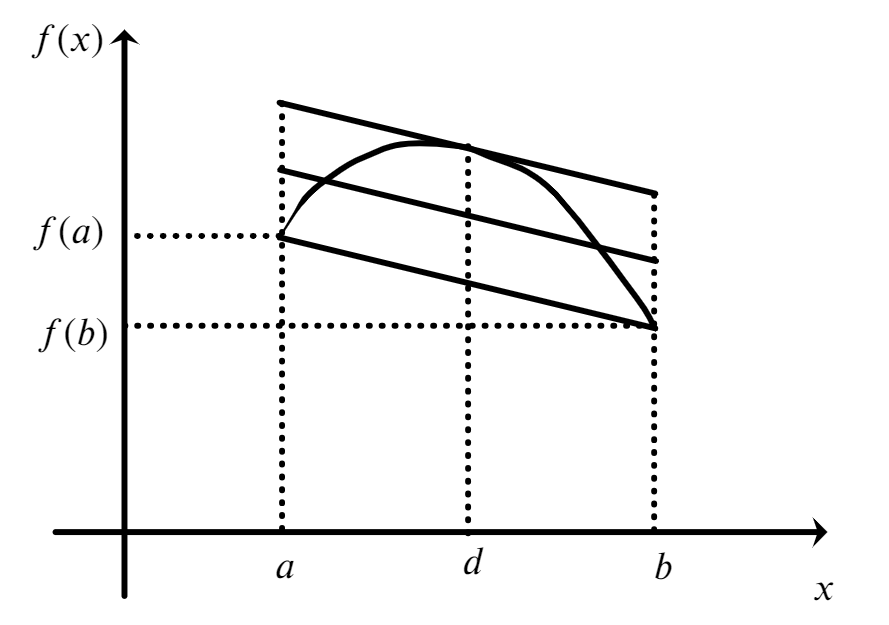
\includegraphics[scale=0.3]{img8}
 	 	$$
 	 	
 	 	 	 \end{enumerate}
 	 	\section{Интерполяционное приближение функции.}
 	 	\subsection{Формулировка задачи интерполирования.}
 	 	$\bullet$ \textit{\textbf{Интерполированием} называется такой способ приближения функции $f(x)$, $x\in [a,b]$ другой функцией $\varphi(x,a)$, где $a = (a_0,\ldots, a_n)$ --- векторный параметр, когда функция $\varphi(x,a)$ определяется из условия совпадения в точках $x_0,\ldots, x_n$, то есть
 	 	$$\varphi(x_i,a_0,\ldots, a_n) = f(x_i),\quad i =0,1,\ldots, n.\eqno(1)$$
 	 	При этом значения $x_i$ называются \textbf{узлами интерполирования}, а совокупность пар чисел $(x_i, f(x_i)), i = \overline{0,n}$ называются \textbf{исходными данными интерполирования}.}\\\\
 	 	Задачу интерполирования можно сформулировать следующим образом. Пусть рассматривается некоторый класс функций $\mathcal F$, где функции $f\in \mathcal F$ заданы на отрезке $[a,b]$, т.е. $f(x)$, $x\in [a,b]$. Для интерполирования $\mathcal F$ выберем семейство функций $\Phi$, состоящее из функций $\varphi \in \Phi$  более простых, чем $f$, и легко вычисляемых. \\\\
 	 	Требуется среди всех функций $\varphi$ найти такую, которая имеет такие же исходные данные интерполирования, что и $f$. Надо выяснить условия существования и единственности решения поставленной задачи. Для определенности будем рассматривать линейную задачу приближения функций, то есть семейство $\Phi$ является линейным подпространством, натянутым на базисные функции $\varphi_i(x)$, $i=\overline{0,n}$. Тогда любая функция $\varphi$ может быть представлена в виде обобщенного многочлена $$\varphi(x) = \sum_{k=0}^n a_k \varphi_k(x),\eqno(2)$$
 	 	$a_k$ --- это константы, подлежащие определению (если мы их найдем, то получим единственную функцию, которая будет совпадать с исходными данными). Параметры $a_k$ выбираются так, чтобы выполнялись условия (1). То есть $$\sum_{k=0}^{n}a_k\varphi_k(x_i) = f(x_i),\quad i =0,1,\ldots, n.\eqno(3)$$
 	 	Для существования и единственности решения данной системы (а значит и задачи интерполирования) необходимо и достаточно, чтобы $$\Delta \equiv \det \{\varphi_k(x_i)\} = \begin{vmatrix}
 	 		\varphi_0(x_0) & \dots & \varphi_n(x_0)\\
 	 		\varphi_0(x_1) & \dots & \varphi_n(x_1)\\
 	 		\vdots & \ddots & \vdots \\
 	 		\varphi_0(x_n) & \dots & \varphi_n(x_n) 
 	 	\end{vmatrix}\ne 0,\quad x_i\ne x_j. \eqno(4)$$
 	 	$\bullet$ \textit{Система функций $\varphi_i$, удовлетворяющая условию (4), называется \textbf{чебышевской}.}\\\\
	Любая система чебышевских функций является линейно независимой, но не каждая линейно независимая система может быть чебышевской.\\\\
	Кроме выполнения условий (4) система функций ${\varphi_i}$ должна обладать свойством полноты.\\\\
	$\bullet$ \textit{Систему функций ${\varphi_i}$ будем называть полной в классе функций $f \in \mathcal F$, если} $$\forall f\in \mathcal F,\ \forall \epsilon > 0\ \exists n_\epsilon : \forall n \geq n_\epsilon\ \exists a_0,\ldots, a_n : \forall x \in [a,b]\quad \Big|f(x) - \sum_{k=0}^{n}a_k\varphi_k|\leq \epsilon.$$
	Таким образом, для решения задачи интерполирования необходимо выполнение следующих требований:
	\begin{enumerate}
		\item система, составленная из функций $\varphi_i(x)$, $i=\overline{0,n}$ должна быть чебышевской системой;
		\item система функций $\{\varphi_i\}$ должна быть полной в рассматриваемом классе функций.
	\end{enumerate}
	\subsection{Алгебраическое интерполирование. Многочлены Лагранжа и Ньютона.}
	В качестве функций $\varphi_i$ будем брать алгебраический базис $$\varphi_i = x^i,\quad i=\overline{0,n}.$$
	Тогда обобщенный многочлен является обычным алгебраическим многочленом $$P_n(x) = \sum_{k=0}^{n}a_kx^k.\eqno(5)$$
	Система функций $x^i$ является чебышевской и полной в классе функций $C[a,b]$. Тогда определитель (4) будет иметь вид $$\Delta = \begin{vmatrix}
		1 & x_0 &\ldots &x_0^n\\
		1 & x_1 &\ldots & x_1^n\\
		\vdots & \vdots & \ddots & \vdots\\
		1 & x_n &\ldots & x_n^n\\
	\end{vmatrix}\ne 0,\quad x _i \ne x_j$$ --- \textbf{определитель Вандермонда}. В данном случае задача интерполирования называется \textbf{задачей алгебраического интерполирования}. Она всегда разрешима единственным образом.\\\\
	Итак интерполяционный многочлен строится по формуле (5), а коэффициенты $a_k$ мы будем искать из системы $$P_n(x_i) = f(x_i),\quad i=\overline{0,n}. \eqno(6)$$
	Если решать эту систему методом Крамера, то коэффициенты можно выразить как $$a_k = \dfrac{\Delta _k}{\Delta}.$$
	Тогда вместо (5) мы получим $$P_n(x) = \dfrac{\Delta_0}{\Delta} + \dfrac{\Delta_1}{\Delta}x +\ldots + \dfrac{\Delta_n}{\Delta}x^n.\eqno(7)$$ 
	Представим многочлен $P_n(x)$ в другой форме. Для этого разложим каждый определитель в уравнении (7) по элементам $i$-ого столбца:
	$$\Delta _i = \sum_{j=0}^{n}f(x_j)\Delta_{ij},$$
	где $\Delta_{ij}$ -- соответствующее алгебраическое дополнение.
	Подставляя выражение в (7) и приведя подобные, мы получим другое представление интерполяционного полинома $$P_n(x) = l_0(x)f(x_0) + l_1(x)f(x_1)+\ldots + l_n(x)f(x_n).\eqno(8)$$
	В формуле (8) $l_i$ являются линейными комбинациями функций $x^j$.
	\subsubsection{Интерполяционный многочлен Лагранжа.}
	Используем простые алгебраические соображения. Так как для полинома (8) должны выполняться условия (6), то $$l_i(x_j) = \delta_{ij}.$$
	Каждый множитель $l_i(x)$ является многочленом $n$-ой степени. Следовательно, его корнями должны являться узлы $x_0,x_1,\ldots, x_{i-1}, x_{i+1},\ldots, x_n$. Так как $l_i(x)$ --- это многочлены $n$-ой степени, то узлы --- это \textit{все} его корни. Тогда мы можем записать $$l_i(x) = c_i(x-x_0)\ldots(x-x_{i-1})(x-x_{i+1})\ldots (x-x_n),$$
	константу $c_i$ вычислим из условия $$l_i(x_i) = 1,$$ отсюда $$c_i = \dfrac{1}{(x_i - x_0)\ldots (x_i - x_{i-1})(x_i - x_{i+1})\ldots (x_i-x_n)}.$$
	Введем в рассмотрение полином $(n+1)$-ой степени $$\omega_{n+1}(x) = (x-x_0)\ldots (x-x_n).\eqno(9)$$
	Тогда $$c_i = \dfrac{1}{w'_{n+1}(x_i)}.$$
	Отсюда мы можем записать формулу 
	$$P_n(x) = \sum_{i=0}^{n}l_i(x)f(x_i) = \sum_{i=0}^{n}\dfrac{w_{n+1}(x)}{(x-x_i)w'_{n+1}(x_i)}f(x_i).\eqno(10)$$
	Формула (10) называется \textbf{формулой Лагранжа для интерполяционного многочлена $P_n$}.\\\\
	\textbf{Замечание}. С помощью формулы Лагранжа легко интерполировать функции, заданные на одной и той же сетке узлов. То есть это более экономичная формула для интерполирования разных функций на одной и той же сетке узлов. Формула (7) же позволяет интерполировать одну и ту же функцию, у которой меняется сетка узлов.
	\subsubsection{Интерполяционный многочлен Ньютона.}
	Получим представление интерполяционного многочлена в виде (7), не вычисляя определитель. Для этого нам понадобится аппарат разделенных разностей. Фактически это математические объекты, которые являются дискретными аналогами производных функции.\\\\
	$\bullet$ \textit{\textbf{Разделенная разность нулевого порядка для функции $f(x)$} совпадают со значениями функции $f(x_i)$ в узлах интерполирования. \textbf{Разделенная разность первого порядка} есть $$f(x_i, x_j) = \dfrac{f(x_j) - f(x_i)}{x_j - x_i}.$$
	\textbf{Разделенная разность второго порядка} $$f(x_i, x_j, x_k) = \dfrac{f(x_j, x_k) - f(x_i, x_j)}{x_k - x_i}.$$ \textbf{Разделенная разность $(k+1)$-ого порядка}} $$f(x_0, \ldots, x_{k+1}) = \dfrac{f(x_1,\ldots, x_{k+1}) - f(x_0,\ldots, x_k)}{x_{k+1} - x_0}.$$
	Можно показать, что справедлива формула, связывающая разделенную разность $k$-ого порядка со значениями функции в указанных узлах
	$$f(x_0, x_1,\ldots, x_k) = \sum_{j=0}^{k} \dfrac{f(x_j)}{\omega_{k+1}'(x_j)},\eqno(11)$$
	где $\omega_{k+1}$ определяется из формулы (9).\\\\
	\textbf{\textit{Свойства разделенных разностей:}}
	\begin{enumerate}
		\item \textit{Разделенная разность любого порядка есть линейный функционал, то есть, если есть линейная функция $g(x) = \alpha f(x) + \beta h(x)$, то разделенная разность от функции $g(x)$ в узлах $x_0,\ldots, x_k$ равна} $$g(x_0,\ldots, x_k) = \alpha f(x_0,\ldots, x_k) + \beta h(x_0,\ldots, x_k).$$
		\item \textit{Разделенная разность есть симметрическая функция своих аргументов $x_0,\ldots, x_k$.}
		\item \textit{Разделенная разность первого порядка от алгебраического многочлена степени $n$ есть алгебраический многочлен степени $n-1$ от тех же значений аргумента (другими словами алгебраическая разность понижает степень полинома). Разделенная разность порядка $n$ от многочлена степени $n$ есть константа, а все разделенные разности более высокого порядка равны нулю.}
	\end{enumerate}
	В практических вычислениях подсчет разделенных разностей реализуется через таблицу
	$$
		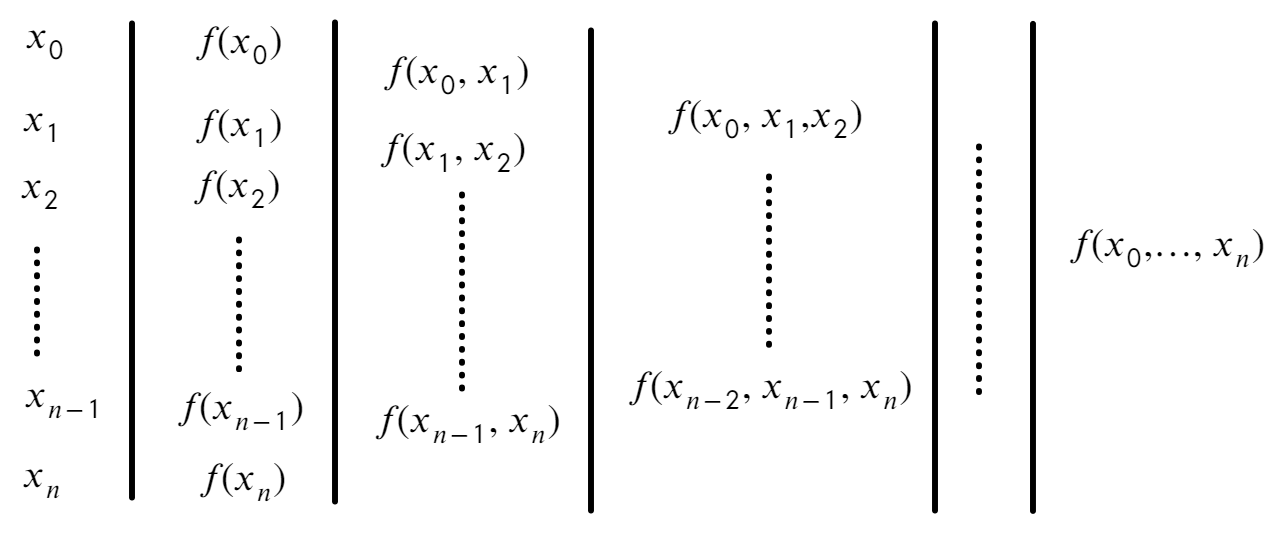
\includegraphics[scale=0.35]{img9}
	$$
	Используя аппарат разделенных разностей получим формулу интерполяционного многочлена. Пусть $P_k(x)$ --- алгебраический многочлен степени $k$ интерполирующий функцию $f(x)$ по узлам $x_0,\ldots, x_k$. Запишем тождественное равенство $$P_n(x) = P_0(x) + [P_1(x) - P_0(x)] + [P_2(x) - P_1(x)] + \ldots + [P_n(x) - P_{n-1}(x)].$$
	Любая разность $P_k(x) - P_{k-1}(x), k=\overline{1,n}$ является многочленом степени $k$. Причем он обращается в ноль в узлах $x_0,\ldots, x_{k-1}$. Следовательно, разность равна $$P_k(x) - P_{k-1}(x) = A_k(x-x_0)\ldots (x-x_{k-1}) = A_k\omega_k(x).$$
	Подставляя в последнее равенство $x = x_k$ и учитывая, что $P_k(x_k) = f(x_k)$, получим $$f(x_k) - P_{k-1}(x_k) = A_k(x_k-x_0)\ldots(x_k - x_{k-1}) = A_k\omega_k (x_k).$$
	Легко видеть, что $$A_k\omega_k(x_k) = A_k\omega_{k+1}'(x_k).$$
	Пользуясь формулой Лагранжа для интерполяционного многочлена, можем переписать полученный результат в виде
	\begin{multline*}
		A_k = \dfrac{f(x_k)}{\omega_{k+1}'(x_k)} - \dfrac{P_{k-1}(x_k)}{\omega_k(x_k)}= \dfrac{f(x_k)}{\omega_{k+1}'(x_k)} - \sum_{j=0}^{k-1}\dfrac{\omega_k(x_k)f(x_j)}{\underbrace{(x_k - x_j)\omega'_k(x_j)}_{-\omega'_{k+1}(x_j)}\omega_k(x_k)}=\\=\dfrac{f(x_k)}{\omega_{k+1}'(x_k)} + \sum_{j=0}^{k-1}\dfrac{f(x_j)}{\omega'_{k+1}(x_j)} =f(x_0,\ldots, x_k).
	\end{multline*}
	А значит $$P_k(x) - P_{k-1}(x) = (x-x_0)\cdot \ldots \cdot (x-x_k)\cdot f(x_0,\ldots, x_k),\quad k=\overline{1,n}.$$
	Подставляя это в формулу для тождественного представления $P_n(x)$, мы в итоге получим
	\begin{multline*}
		P_n(x) = f(x_0) + (x-x_0)\cdot f(x_0, x_1) + (x-x_0)(x-x_1)\cdot f(x_0,x_1,x_2) +\ldots \\ \ldots + (x-x_0)\ldots (x-x_{n-1})\cdot f(x_0,\ldots, x_n).\quad(12)
	\end{multline*}
	$\bullet$ \textit{Формула $(12)$ называется \textbf{формулой Ньютона для интерполяционного многочлена} $P_n(x)$. А сам многочлен, определяемый формулой $(12)$ называется \textbf{интерполяционным многочленом Ньютона}.}
	\subsection{Остаток интерполирования.}
	$\bullet$ \textit{Под \textbf{остатком интерполирования} будем понимать разность} $$r_n(x) = f(x) - P_n(x).$$
	Величина $r_n(x)$ зависит от следующих факторов:
	\begin{enumerate}
		\item от свойств интерполируемой функции $f(x)$;
		\item от выбора узлов интерполирования $x_0,\ldots,x_n$;
		\item выбора точки интерполирования $x$.
	\end{enumerate}
	\subsubsection{Представления остатка интерполирования.}
	Рассмотрим разделенную разность $(n+1)$-ого порядка $f(x,x_0,\ldots,x_n)$ и применим к ней формулу (11), тогда получим
	\begin{multline*}
		f(x,x_0,\ldots,x_n) = \dfrac{f(x)}{(x-x_0)\ldots (x-x_n)} + \dfrac{f(x_0)}{(x_0-x)(x_0-x_1)\ldots(x_0-x_n)} + \ldots \\ \ldots + \dfrac{f(x_n)}{(x_n-x)(x_n-x_0)\ldots (x_n-x_{n-1})} = \dfrac{f(x)}{\omega_{n+1}(x)} + \sum_{j=0}^{n}\dfrac{f(x_j)}{(x_j-x)\cdot \omega_{n+1}'(x_j)}.
	\end{multline*}
	Выразим $f(x)$ из последнего равенства $$f(x) = \omega_{n+1}'(x)\cdot f(x,x_0,\ldots, x_n) + \underbrace{\sum_{j=0}^{n}\dfrac{\omega_{n+1}'(x)\cdot f(x_j)}{(x-x_j)\cdot \omega_{n+1}'(x_j)}}_{P_n(x)},$$
	где $P_n(x)$ задано по формуле Лагранжа. Отсюда следует, что $$r_n(x) = \omega_{n+1}(x)\cdot f(x,x_0,\ldots, x_n).\eqno(13)$$
	$\bullet$ \textit{Формула $(13)$ --- это \textbf{представление остатка интерполирования в форме Ньютона}.}\\\\
	Получим представление в форме Лагранжа. Для этого сделаем предположение о свойствах дифференцируемости функции, то есть предположим, что $f(x)\in C^{n+1}[a,b]$. Введем в рассмотрение вспомогательную функцию $$\varphi(t) = f(t) - P_n(t) - k\omega_{n+1}(t),\quad k = \operatorname{const}.$$
	Очевидно, что в узлах интерполирования $$\varphi(x_0) = \varphi(x_1)=\ldots = \varphi(x_n) = 0.$$
	Подберем $k$ таким образом, чтобы функция обращалась в ноль и в точке интерполирования $t=x$. То есть должно выполняться условие $$\varphi(x) = f(x) - P_n(x) - k\omega_{n+1}(x) = 0.$$
	Отсюда $$k = \dfrac{r_n(x)}{\omega_{n+1}(x)},$$
	причем знаменатель отличен от нуля, потому что точка $x$ не является узлом интерполирования $x_i$, $i=\overline{0,n}$.
	Из этой формулы следует $$r_{n+1}(x) = k\omega(x).\eqno(14)$$ При таком способе задания функции $\varphi$ можно утверждать, что $\varphi \in C^{n+1}[a,b]$, обращается в ноль на $[a,b]$ в $(n+2)$-ух точках $x,x_0,\ldots, x_n$. По теореме Ролля производная $\varphi'(t) = 0$ по крайней мере в $n+1$ точке. Применяя далее теорему Ролля к $\varphi'(t)$, получим, что вторая производная $\varphi''(t) = 0$ в $n$ точках. И так далее получим, что существует по крайней мере одна точка $\xi\in (a,b)$ такая, что $$\varphi^{(n+1)}(\xi) = 0.$$
	С другой стороны, $$\varphi^{(n+1)}(t) = f^{(n+1)}(t) - k\omega_{n+1}^{(n+1)}(t).$$
	В свою очередь $\omega^{(n+1)}_{n+1}(t) = (n+1)!$. Подставляем $t=\xi$ и находим $k$ $$k=\dfrac{f^{(n+1)}(\xi)}{(n+1)!}.$$
	Подставляем это значение $k$ в формулу (14) и получим $$r_n(x) = \omega_{n+1}(x) \dfrac{f^{(n+1)}(\xi)}{(n+1)!},\quad \xi \in [a,b].\eqno(15)$$
	$\bullet$ \textit{Формула $(15)$ называется \textbf{представлением остатка интерполирования в форме Лагранжа}.}\\\\
	Формула (15) позволяет решить задачу об оценке величины погрешности в любой точке отрезка 
	$$|r_n(x)| \leq |\omega_{n+1}(x)| \dfrac{\underset{x\in[a,b]}{\max} |f^{(n+1)}(x)|}{(n+1)!}.$$
	Из формул (13) и (15) можно получить связь между разделенной разностью $n$-ого порядка и ее производной $$f(x_0,\ldots, x_n) = \dfrac{f^{(n)}(\xi)}{n!},\quad \xi\in[a,b].\eqno(16)$$
	\subsubsection{Минимизация остатка интерполирования. Многочлены Чебышева.}
	Рассмотрим вопрос о точности интерполирования функции. Если интерполируется одна определенная функция $f(x)$, то точность интерполирования характеризуется величиной $$\max_{x\in[a,b]}|r_n(x)|.$$
	Когда мы интерполируем не одну функцию, а некоторое множество функций, то точность может быть оценена величиной $$\sup_f\max_{x\in[a,b]}|r_n(x)|.$$
	Поставим задачу о выборе узлов $x_i$, которые можно было бы считать наилучшими при интерполировании всех функций $f(x)$, $x\in [a,b]$ из взятого множества. Такими узлами естественно считать те, для которых величина $\sup\max$ достигает наименьшего значения. \\\\
	Пусть функция $f(x)\in C^{n+1}[a,b]$ и для нее выполняется неравенство $$|f^{(n+1)}(x)|\leq M, \quad x\in [a,b].$$
	Тогда погрешность интерполирования может быть оценена сверху следующим образом $$\max_x |r_n(x)| \leq \dfrac{M}{(n+1)!}\max_x|\omega_{n+1}(x)|$$
	(эта оценка является наилучшей). Тогда $$\sup_f\max_{x\in[a,b]}|r_n(x)| = \dfrac{M}{(n+1)!}\cdot \max_x |\omega_{n+1}(x)|.$$
	Поэтому наилучшими узлами при интерполировании функции $f(x)$ являются те, для которых $$\max_{x\in [a,b]}|\omega_{n+1}(x)|=\min.$$
	При этом и величина остатка интерполирования будет минимальной для любой функции $f$ из рассматриваемого класса.
	Задача о минимизации остатка интерполирования сводится к построению приведенного алгебраического многочлена $(n+1)$-ой степени, наименее отклоняющегося от нуля на отрезке $[a,b]$, причем корни этого многочлена вещественны, различны и принадлежат отрезку $[a,b]$.\\\\
	$\bullet$ \textit{\textbf{Многочленами Чебышева} будем называть множество многочленов $T_n(x)$, $n\geq 0$, определяемых соотношениями} $$T_0(x)=1,\ T_1(x) = x,\ T_{n+1}(x) = 2xT_n(x) - T_{n-1}(x),\quad n=1,2,\ldots. \eqno(17)$$
	\textbf{\textit{Свойства многочленов Чебышева:}}
	\begin{enumerate}
		\item \textit{Старший член многочлена $T_n(x)$ при $n > 0$ есть $2^{n-1}x^n$}.
		\item \textit{Все многочлены $T_{2n}(x)$ --- четные функции, а $T_{2n+1}(x)$ --- нечетные функции.}
		\item $T_{2n}(x) = 2T_n^2(x) - 1$.
		\item \textit{Многочлены Чебышева образуют ортогональную по весу $p(x) = \dfrac{1}{\sqrt{1-x^2}}$ на отрезке $[-1, 1]$ систему многочленов.}
	\end{enumerate}
	$$T_n(x) = \cos(n\arccos x), n\geq 0 \eqno(18)$$ --- тригонометрическая форма представления многочленов Чебышева.\\\\
	Из формулы (18) легко видеть, что $|T_n(x)|\leq 1$, $|x| \leq 1$, а корнями этого многочлена являются значения $$x_k = \cos \dfrac{\pi (2k+1)}{2n}, k =\overline{0,n-1}.\eqno(19)$$
	Из формулы (18) легко получить точки экстремума многочленов Чебышева $$x_k^* = \dfrac{\cos \pi k}{n}, k=\overline{0,n},$$
	при этом значения полинома в этих точках $$T_n(x_k^*) = \cos\pi k =(-1)^k.$$
	Приведенные многочлены Чебышева $$\overline T_n(x) = 2^{1-n}T_n(x).$$
	Если мы возьмем в качестве $\omega_{n+1}$ приведенный многочлен Чебышева, то он будет наименее отклоняющимся от нуля.
	\begin{theorem}
		Если $P_n(x)$ --- многочлен степени $n$ со старшим коэффициентом равным единице, то $$\max_{x\in [-1,1]}|P_n(x)|\geq \max_{x\in [-1,1]} |\overline T_n(x)|$$
	\end{theorem}
	\begin{Proof}
		Без доказательства.
	\end{Proof}\\\\
	Для решения задачи минимизации остатка интерполирования в качестве $\omega_{n+1}$ надо взять многочлен Чебышева минимально отклоняющийся от нуля на отрезке $[a,b]$.\\\\ Получим вид многочлена Чебышева на отрезке $[a,b]$, сделав замену $$x' = \dfrac{b+a}{2} + \dfrac{b-a}{2}x,\quad x \in [-1, 1],\ x' \in [a,b].$$
	Применяя эту замену переменных, в качестве $\omega_{n+1}(x)$ надо взять многочлены Чебышева следующего вида: $$T_{n+1}(x) = \dfrac{(b-a)^{n+1}}{2^{2n+1}} \cos\Big((n+1)\arccos \dfrac{2x - (b+a)}{b-a}\Big),\ x\in [a,b]\eqno(20)$$
	Запишем, чему равны корни многочлена $(20)$:
	$$x_k = \dfrac{a+b}{2} + \dfrac{b-a}{2}\cos \dfrac{(2k+1)\pi}{2(n+1)},\ k=\overline{0,n}.\eqno(21)$$
	Если выбрать узлами интерполирования $x_0,\ldots, x_n$, совпадающие с корнями полинома $(21)$, то величина отклонения $\omega_{n+1}(x)$ от нуля окажется минимальной. Максимальное же значение этого отклонения равно $$\max_{x \in [a,b]} |\omega_{n+1}(x)|=\dfrac{(b-a)^{n+1}}{2^{2n+1}}.$$
	При этом справедлива оценка для погрешности $$|r_n(x)| \leq \dfrac{M}{(n+1)!}\cdot \dfrac{(b-a)^{n+1}}{2^{2n+1}}.\eqno(22)$$
	Для упорядочивания узлов необходима перенумерация $\widetilde{x}_k = x_{n-k},\ k=\overline{0,n}.$
	\subsection{Интерполирование при равноотстоящих узлах.}
	Пусть функция $f(x)$ задана таблично в точках $x_i$, которые являются равноотстоящими, то есть $$x_i = x_i + ih,\ h>0, i = 0,1,\ldots$$
	Рассмотрим вместо разделенных разностей аппарат конечных разностей.\\\\ 
	$\bullet$ \textit{\textbf{Конечная разность нулевого порядка} совпадает со значением функции $f(x_i) = f_i$.
	\textbf{Конечная разность первого порядка} определяется равенствами  $$\Delta f_i = f_{i+1} - f_i.$$ \textbf{Конечная разность второго порядка} определяется равенствами $$\Delta^2 f_i = \Delta f_{i+1} - \Delta f_{i}.$$
	\textbf{Конечная разность $k$-ого порядка} определяется равенствами} $$\Delta ^k f_i = \Delta (\Delta^{k-1} f_i) = \Delta ^{k-1}f_{i+1} - \Delta ^{k-1}f_i.$$
	Очевидно, что аппарат конечных разностей является частным случаем аппарата разделенных разностей.\\\\
	Можно получить формулу для конечной разности первого порядка $$\Delta ^k f_i = \sum_{j=0}^{k}(-1)^j C^j_k f_{i+k-j},\eqno(23)$$
	где $C_k^j$ --- коэффициенты бинома Ньютона.\\\\
	Свойства конечных разностей совпадают со свойствами разделенных разностей, кроме симметрии. Вычисления конечных разностей производится в виде таблицы
	$$
		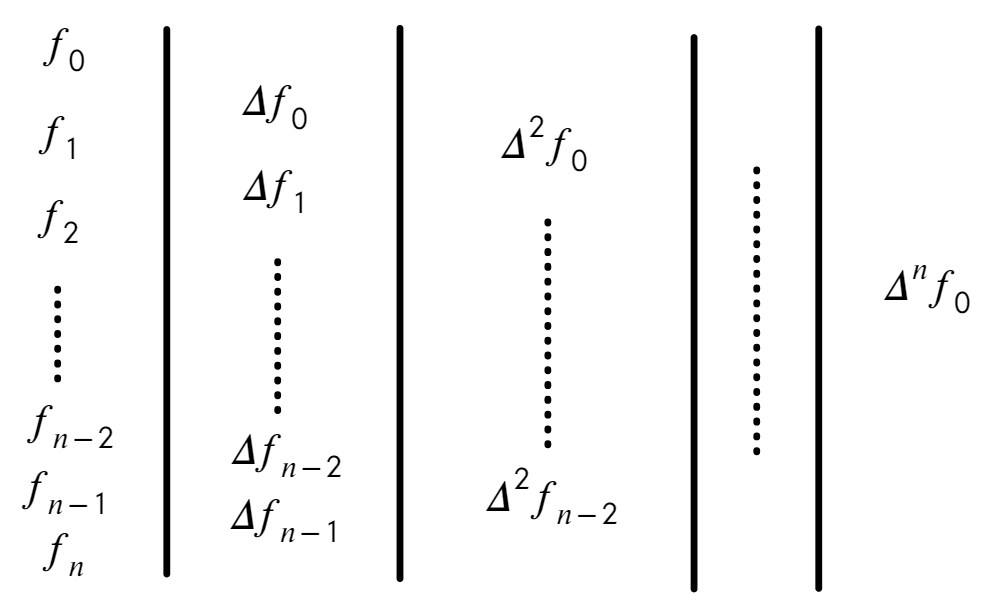
\includegraphics[scale=0.35]{img10}
	$$
	Запишем формулу, которая устанавливает взаимосвязь между разделенными и конечными разностями $$f(x_0,\ldots, x_k) = \dfrac{\Delta^k f_0}{k! h^k}.\eqno(24)$$
	Аналогично формуле (16), можно записать формулу для связи между конечной разностью $k$-ого порядка и производной $k$-ого порядка $$\Delta^k f_0 = h^k f^{(k)}(\xi),\ \xi \in [x_0, x_0 + kh].\eqno(25)$$
	Из формулы (25) следует, что при малом шаге $h<1$ $$\Delta^kf_0 =\begin{cases}
		O(h^k), \quad f^{(k)}(\xi) \ne 0,\\
		o(h^k), \quad f^{(k)}(\xi) = 0.\\
	\end{cases} $$
	Это означает, что для достаточно гладкой функции ее конечные разности уже не очень высокого порядка оказываются достаточно малыми величинами.\\\\
	Предположим, что значения $f_i$ вычислены с погрешностью $$f_i = \widetilde{f}_i + \delta _i.$$
	Используя формулу (23), получим $$\Delta^kf_0 = \sum_{j=0}^{k} (-1)^j C^j_k f_{k-j} = \sum_{j=0}^{k} (-1)^j C^j_k (\widetilde f_{k-j} + \delta_{k-j})= \Delta^k \widetilde f _0 + \sum_{j=0}^{k} (-1)^j C^j_k \delta_{k-j},\ j=\overline{0,k}.$$
	Оценим погрешность $$\Big| \sum_{j=0}^{k} (-1)^j C^j_k \delta_{k-j}\Big| \leq [|\delta_i|\leq \delta] \leq \delta \sum_{j=0}^{k} C_k^j = \delta \cdot 2^k.$$
	Таким образом, $$\Delta^kf_0= \Delta^k \widetilde f _0 + 2^k \delta.$$
	Если точные значения конечных разностей будут убывать, то приближенные значения будут увеличиваться. 
	\subsubsection{Интерполирование в начале таблицы.}
	Пусть $x \in [x_0, x_1]$. Будем предполагать, что для достижения требуемой точности достаточно интерполирования многочленом $k$-ой степени и для этого возьмем $k+1$ узлов $$x_0, x_0+h,\ldots, x_0+kh.$$
	Применим формулу (12) к равномерной сетке узлов $$P_n(x) = f(x_0) + (x-x_0)f(x_0, x_0+h) +\ldots + (x-x_0)\ldots (x-x_0-kh + h)f(x_0,x_0+h,\ldots, x_0 + kh).$$
	Произведем замену переменных по формуле $$t = \dfrac{x-x_0}{h}.$$ После этого заменим разделенную разность на конечную разность по формуле (24). В итоге получим выражение $$P_k(x) = P_k(x+th) = f_0 + \dfrac{t}{1!}\Delta f_0 + \dfrac{t(t-1)}{2!} \Delta^2f_0 + \ldots + \dfrac{t(t-1)\ldots (t-k+1)}{k!}\Delta^k f_0\eqno(26)$$
	$\bullet$ \textit{Формула $(26)$ называется \textbf{правилом интерполирования в начале таблицы}, а полином $P_k(x)$ называется \textbf{интерполяционным многочленом Ньютона для начала таблицы}.}\\\\
	Аналогично выражению для остатка интерполяционного многочлена Ньютона, мы можем записать выражение для остатка многочлена Ньютона в начале таблицы $$r_k(x) = r_k(x_0 + th) = h^{k+1} \dfrac{t(t-1)\ldots (t-k)}{(k+1)!}f^{(k+1)}(\xi),\ \xi \in [x_0, x_0 + kh],\ t\in [0,1].\eqno(27)$$
	\subsubsection{Интерполирование в конце таблицы.}
	Пусть точка интерполирования находится в конце таблицы $x\in[x_{n-1}, x_n]$. В качестве узлов интерполирования возьмем узлы $x_n, x_{n-1}, \ldots, x_{n-k}$, но, учитывая, что узлы равномерные, то $$x_n, x_n-h,\ldots, x_n-kh.$$
	В силу этих обозначений запишем интерполирующий полином $k$-ой степени Ньютона по заданным узлам \begin{multline*}
		P_k(x) = f(x_n) + (x-x_n)f(x_n, x_n-h) + (x-x_n)(x - x_n + h)f(x_n, x_n - h, x_n-2h) +\\+ \ldots + (x-x_n)(x-x_n + h)\ldots (x-x_n + kh - h)f(x_n, x_n -h,\ldots, x_n-kh).
	\end{multline*}
	Сделаем замену $$t = \dfrac{x-x_n}{h},\quad t\in [-1, 0].$$
	Примем по внимание тот факт, что разделенные разности можно выразить через конечные разности, учитывая равномерную сетку. Разделенная разность $i$-ого порядка выражается через конечную разность $i$-ого порядка относительно точки $f_{n-i}$ следующим образом $$f(x_n, x_n-h,\ldots, x_n - ih) = \dfrac{\Delta^i f_{n-i}}{i! h^i}.$$
	После замены получим полином $$P_k(x) = P_k(x_n + th) = f_n + \dfrac{t}{1!}\Delta f_{n-1} + \dfrac{t(t+1)}{2!}\Delta^2f_{n-2} + \ldots + \dfrac{t(t+1)\ldots (t+k-1)}{k!}\Delta^k f_{n-k}\eqno(28)$$
	$\bullet$ \textit{Формула $(28)$ называется \textbf{правилом интерполирования в конце таблицы}. А полином $P_k(x)$ называется \textbf{интерполяционным многочленом Ньютона для конца таблицы.}}\\\\
	Так же, как и в предыдущем случае, остаток интерполирования будет равен $$r_k(x) = r_k(x_n + th) = h^{k+1}\dfrac{t(t+1)\ldots (t+k)}{(k+1)!}f^{(k+1)}(\xi),\ \xi \in [x_n, x_{n}-kh].\eqno (29)$$
	\subsubsection{Интерполирование внутри таблицы.}
	Пусть $x_n$ --- внутренний узел, в окрестности которого находится точка интерполирования, а $x$ --- точка интерполирования.
	Различают два варианта
	\begin{enumerate}
		\item Пусть $|x-x_n| < \dfrac{h}{2}$, то есть точка интерполирования находится в окрестности полушага. Тогда табличные узлы целесообразно привлекать к порядку удаленности от $x_n$, то есть "парами": $$x_n, (x_n - h, x_n+h), (x_n-2h, x_n + 2h), \ldots, (x_n - kh, x_n + kh)$$
		Число узлов при этом будет нечетным $2k+1$, а полином будет иметь четную степень $2k$. Поэтому при таком порядке можно получить следующее правило \begin{multline*}
			P_{2k}(x) = P_{2k}(x+th) = f_n + \dfrac{t}{1!}\cdot \dfrac{\Delta f_n + \Delta f_{n-1}}{2}+ \dfrac{t^2}{2!}\cdot \Delta ^2 f_{n-1} + \dfrac{t(t^2 - 1^2)}{3!}\cdot\dfrac{\Delta ^3 f_{n-1}+\ldots \Delta^3 f_{n-2}}{2} +\ldots \\ +\ldots + \dfrac{t^2(t^2 - 1^2)\ldots (t^2 - (k-1)^2)}{2k!}\cdot \Delta^{2k}f_{n-k}. \quad (30) 
		\end{multline*}
		$\bullet$ \textit{Формула $(30)$ называется \textbf{правилом Ньютона-Стирлинга интерполирования внутри таблицы}.}\\\\
		Остаток интерполирования будет выглядеть следующим образом $$r_{2k}(x) = r_{2k}(x_n + th) = h^{2k+1} \dfrac{t^2(t^2-1^2)\ldots (t^2 - k^2)}{(2k+1)!}\cdot f^{(2k+1)}(\xi),\ \xi \in [x_n - kh, x_n + kh].\eqno (31)$$
		\item Пусть точка $x$ лежит вблизи середины отрезка между двумя соседними внутренними узлами, то есть $x\in [x_n, x_n + h]$, $x\approx x_n + \dfrac h2$. Пусть для интерполирования привлекаются следующие пары узлов $$(x_n, x_n + h), (x_n - h, x_n + 2h), \ldots, (x_n-kh + h, x_n + kh).$$
		Число узлов при этом будет четным $2k$, а полином будет иметь нечетную степень $2k-1$. 
		\begin{multline*}
			P_{2k-1}(x) = P_{2k-1}(x+th) = \dfrac{f_n + f_{n+1}}{2} + \dfrac{t-\frac12}{1!}\Delta f_n +\\+ \dfrac{t(t-1)}{2!}\cdot \dfrac{\Delta^2 f_n + \Delta^2 f_{n-1}}{2} + \dfrac{t(t-1)(t-\frac12)}{3!} \Delta^3 f_{n-1} + \ldots \quad (32)
		\end{multline*}
		$\bullet$ \textit{Формула $(32)$ называется \textbf{правилом Ньютона-Бесселя интерполирования внутри таблицы}}.\\\\
		Остаток интерполирования правила Ньютона-Бесселя равен
		$$r_{2k-1}(x) = r_{2k-1}(x_n + th) = h^{2k} \dfrac{t(t^2-1^2)\ldots (t^2 - (k-1)^2)}{(2k)!} f^{(2k)}(\xi),\ \xi \in [x_n - kh + h,x_n + kh].\eqno (33)$$
	\end{enumerate}
	\textbf{Замечание.} Формулы интерполирования на равноотстоящих узлах используются для построения табличных значений некоторой функции так, чтобы погрешность интерполяции некоторой функции многочленом заданной степени $m$ не превосходила величины $\epsilon$. То есть, выбираем шаг интерполирования $h$ так, чтобы при заданной степени полинома $|r(x)| \leq \epsilon$.
	\subsection{Интерполирование с кратными узлами.}
	Ранее мы предполагали, что узлы пронумерованы в порядке возрастания, они все различны и их кратность равна единице.
	\subsubsection{Формулировка задачи кратного интерполирования.}
	Пусть на отрезке $[a,b]$ заданы $n+1$ различных узлов $x_0, x_1,\ldots, x_m$. В каждой из этих точек известны значения интерполирования функции $f(x_k)$, а также ее производные $$f'(x_k),\ldots, f^{(\alpha _ k -1)}(x_k),\quad k=\overline{0,m}.$$
	$\bullet$ \textit{Числа $\alpha_0,\alpha_1,\ldots, \alpha _m$ называются \textbf{кратностями узлов} $x_0,x_1,\ldots, x_m$.}\\\\
	Общее число всех исходных данных о функции $f(x)$ обозначим $$\alpha_0 + \alpha_1 + \ldots + \alpha_m = n+1.$$
	В частности, если все $\alpha_k = 1$, $k=\overline{0,m}$, то мы получаем, что все корни простые, а $m=n$. А тогда мы получаем ту же задачу, что решали ранее.\\\\
	Задача ставится следующим образом. Требуется найти такой многочлен $$P_n(x) = a_0x^n + a_1x^{n-1} + \ldots + a_n$$
	 степени не выше $n$, удовлетворяющий условиям $$P^{(j)}_n(x_k) = f^{(j)}(x_k),\quad j =\overline{0,\alpha_k-1}, k = \overline{0,m}. \eqno(34)$$
	 Условия (34) представляют собой систему линейных алгебраически уравнений для определения коэффициентов многочлена. Для доказательства существования и единственности решения этой системы рассмотрим соответствующую однородную систему $$P_n^{(j)}(x_k) = 0,\quad j =\overline{0,\alpha_k-1}, k = \overline{0,m}. \eqno(35)$$ и покажем, что она имеет только нулевое решение. Действительно, если справедливо соотношение (35), то это значит, что узлы интерполирования $x_0,x_1,\ldots, x_{m}$ должны быть корнями полинома $P_n$ кратности не меньше, чем $\alpha_0,\alpha_1,\ldots, \alpha_m$ соответственно.
	 Сумма кратностей должна быть больше или равна $\alpha_0 + \alpha_1 + \ldots + \alpha_m = n+1.$ Но степень $P_n(x)$ не выше $n$. Поэтому сумму кратностей корней большую, чем $n$, многочлен $P_n(x)$ может только в том случае, когда он равен нулю, то есть его коэффициенты равны нулю.
	 А следовательно, система (35) имеет только нулевое решение.\\\\
	 $\bullet$ \textit{Интерполяцию с кратными узлами называют \textbf{Эрмитовой}. А соответствующий алгебраический многочлен $n$-ой степени называется \textbf{интерполяционным многочленом Эрмита}}. 
	 \subsubsection{Интерполяционный многочлен Эрмита и его остаток.}
	 Для получения представления Эрмита воспользуемся представлением (8). Для этого построим многочлены $H_{ij}(x)$ степени не выше $n$, удовлетворяющие условиям $$\begin{cases}
	 H_{ij}(x_k) = H'_{ij}(x_k) = \ldots = H_{ij}^{(\alpha_k-1)}(x_k) = 0,\quad k \ne i,\\
	 H_{ij}(x_i) = H'_{ij}(x_i) = \ldots = H_{ij}^{(j-1)}(x_i) = H_{ij}^{(j+1)}(x_i) = \ldots = H_{ij}^{(\alpha_i - 1)}(x_i) = 0,\\
	 H_{ij}^{(j)}(x_i) = 1,\quad i=\overline{0,m},\ j = \overline{0,\alpha_i-1}.
	 \end{cases}\eqno(36)$$
	 Тогда можно записать следующее представление для интерполяционного многочлена Эрмита $$P_n(x) = \sum_{i=0}^n \sum_{j=0}^{\alpha_i-1}H_{ij}(x) f^{(j)}(x_i).\eqno(37)$$
	 Остаток интерполирования Эрмита записывается по формуле $$r_n(x) = \Omega(x) \dfrac{f^{(n+1)}(\xi)}{(n+1)!},\quad \Omega (x) = (x-x_0)^{\alpha_0}\ldots (x-x_m)^{\alpha_m},\ \xi \in [a,b].\eqno(38)$$
	 Вычислить в явном виде функции $H_{ij}$ достаточно сложно. В силу этого в вычислительной практике явное выражение для полинома (37) не используется. Укажем два простейших частных случая явного представления многочлена Эрмита.
	 \begin{enumerate}
	 	\item Пусть $m = 0$, $\alpha_0 = n+1$. В этом случае $$H_{ij}(x) =\dfrac{1}{j!}(x-x_0)^j.$$
	 	Тогда формула (37) будет иметь вид $$P_n(x) = \sum_{j=0}^n \dfrac{1}{j!}(x-x_0)^j f^{(j)}(x_0).$$
	 	Мы получили выражение для $n$-ой частной суммы ряда Тейлора. Аналогично можно записать $$r_n(x) =(x-x_0)^{n+1} \dfrac{f^{(n+1)}(\xi)}{(n+1)!},$$ который является остаточным членом ряда Тейлора в форме Лагранжа.
	 	\item Пусть $\alpha_0 = \alpha_1 = \ldots = \alpha_m = 2$. В этом случае видно, насколько усложняются расчеты: $$P_n(x) = \sum_{i=0}^m\left[\dfrac{\omega_{m+1}(x)}{(x-x_i)\omega'_{m+1}(x_i)}\right]^2 \left\{ \left[1 - (x-x_i)\dfrac{\omega''_{m+1}(x)}{\omega'_{m+1}(x_i)}\right]f(x_i) + (x-x_i)f'(x_i)\right\}.$$
	 	Остаток в данном случае будет иметь вид $$r_n(x) = \omega_{m+1}^2 \dfrac{f^{(2m+2)}(\xi)}{(2m+2)!}.$$
	 \end{enumerate}
	 Аппарат разделенных разностей помогает без явного выражения коэффициентов, определяющих полином, производить расчеты, чтобы вычислять значения интерполяционного многочлена Эрмита.\\\\
	 Введем понятие разделенной разности с кратными узлами. \\\\
	 $\bullet$ \textit{\textbf{Разделенная разность нулевого порядка} равна $$f(\underbrace{x_0,x_0,\ldots,x_0}_{j+1}) = \lim\limits_{\epsilon\to 0} f(x_{00}^\epsilon, x_{01}^\epsilon,\ldots, x_{0j}^\epsilon),$$ где все узлы $x_{0j}$ различны и $$\lim\limits_{\epsilon\to 0} x_{0i}^\epsilon = x_0,\quad i = \overline{0,j}.$$
	 $\bullet$\textbf{Разделенная разность $p$-ого порядка} равна $$f(\underbrace{x_0,\ldots, x_0}_{j_0}; \ldots; \underbrace{x_p,\ldots, x_p}_{j_p}) = \dfrac{f(\overbrace{x_0,\ldots, x_0}^{j_0-1}; \ldots; \overbrace{x_p,\ldots, x_p}^{j_p}) - f(\overbrace{x_0,\ldots, x_0}^{j_0}; \ldots; \overbrace{x_p,\ldots, x_p}^{j_p-1})}{x_p - x_0}.$$}
	 Таким образом, имеются узлы интерполирования $$x_{00}^\epsilon,\ldots, x_{0\alpha_0 - 1}^\epsilon, \ldots x_{n0}^\epsilon,\ldots, x_{n\alpha_n - 1}^\epsilon,$$ и по этим узлам мы можем построить интерполяционный многочлен Ньютона. Переходя в нем к пределу при $\epsilon \to 0$, мы можем получить представление многочлена Эрмита через разделенные разности
	 \begin{multline*}
	 	P_n(x) = f(x_0) + (x-x_0)f(x_0, x_0) + \ldots + (x-x_0)^{\alpha_0-1}f(x_0,\ldots, x_0) + \\ + (x-x_0)^{\alpha_0}f(x_0,\ldots, x_0; x_1)+ (x-x_0)^{\alpha_0}(x-x_1)f(x_0,\ldots, x_0; x_1, x_1) +\ldots +\\+ \ldots + (x-x_0)^{\alpha_0}(x-x_1)^{\alpha_1-1} f(x_0,\ldots, x_0; x_1,\ldots, x_1) + \ldots+ \\\ +\ldots + (x-x_0)^{\alpha_0}(x-x_1)^{\alpha_1}\ldots(x-x_m)^{\alpha-1}f(x_0,\ldots x_0; x_1,\ldots, x_1; \ldots; x_{m},\ldots, x_{m}).\quad (39)
	 \end{multline*}
	 \textbf{Замечание.} Следует иметь ввиду, что для построения таблицы разделенных разностей, необходимо учитывать соотношение $$f(\underbrace{x_0,\ldots, x_0}_{j+1}) = \dfrac{f^{(j)}(x_0)}{j!}.\eqno(40)$$
	 \subsection{Сплайн-интерполирование.}
	 \subsubsection{Понятие сплайн-функции и интерполяционного сплайна.}
	 Разобъем отрезок $[a,b]$, на котором ищется приближение функции $f(x)$ на $n$ частей точками $$a=x_0 < x_1 < \ldots < x_N = b.$$
	 Обозначим через $h_i=x_i - x_{i-1}$, $i=\overline{1,N}$ расстояние между $i$-ым и $(i-1)$-ым узлами.\\\\ 
	 $\bullet$ \textit{\textbf{Сплайн-функцией $m$-ого порядка} называется функция $S_m(x)$, которая удовлетворяет следующим условиям:}
	 \begin{enumerate}
	 	\item \textit{На каждом из отрезков $[x_{i-1}, x_i]$, $i=\overline{1,N}$ функция $S_m(x)$ является алгебраическим многочленом степени $m$, то есть} $$S_m(x) = P_{im}(x) = a_{i0} + a_{i1}x + \ldots + a_{im}x^m,\quad x\in [x_{i-1}, x_i],\ i=\overline{1,N}.\eqno(41)$$
	 	\item \textit{Функция $S_m(x)$ непрерывна вместе со своими производными до $(m-1)$-ого порядка включительно во всех внутренних точках, в том числе и в точках $x_i$, $i=\overline{1,N-1}$. То есть $$S_m^{(j)}(x_i+0) = S_m^{(j)}(x_i-0),\quad j=\overline{0, m-1}, \ i=\overline{1, N-1}.\eqno(42)$$}
	 \end{enumerate}
	 Условия 1, 2 достаточны для того, чтобы определить сплайн-функцию $m$-ого порядка. \\\\
	 $\bullet$ \textit{Если добавить к этому определению третье условие}
	 \begin{enumerate}
	 	\item [3.] $$S_m(x_i) = f(x_i),\ i=\overline{0,N} \eqno(43)$$
	 \end{enumerate}
	 \textit{то функция $S_m(x)$ называется \textbf{интерполяционным сплайном.}}\\\\
	 Количество неизвестных коэффициентов $a_{ij}$, $i=\overline{1,N}$, $j=\overline{0,m-1}$ из формулы (41) равно $N(m+1)$. Из формулы (42) мы имеем $m(N-1)$ условие и из формулы (43) мы имеем $(N+1)$ условие. Суммируя, получим $N(m+1) - (m-1)$ условие. Таким образом, для однозначного определения сплайна не хватает $(m-1)$ условия. Обычно эти недостающие условия задаются либо на концах отрезка, либо из дополнительной информации о функции.\\\\
	 Далее будем рассматривать случай $m=3$. В вычислительной практике такие сплайны называются кубическими сплайнами, или сплайнами третьего порядка.
	 \subsubsection{Построение кубического сплайна.}
	 Легко увидеть, что на каждом отрезке вторая производная функции $S_3(x)$ представляет собой линейную функцию. Обозначим $$M_i = S''_3(x_i),\quad i = \overline{0,N}.$$
	 Тогда мы можем аналитически записать вторую производную $$S''_3(x) = P_{i3}''(x) = M_{i-1}\dfrac{x_i-x}{h_i} + M_i\dfrac{x - x_{i-1}}{h_i},\quad x \in [x_{i-1}, x_i],\ i = \overline{1,N}.\eqno(44)$$
	 Видно, что соотношение (44) говорит о непрерывности второй производной во всех внутренних узлах $x_i$, а также равенстве второй производной сплайна значению $M_i$ во всех точках $x_i$.
	 $$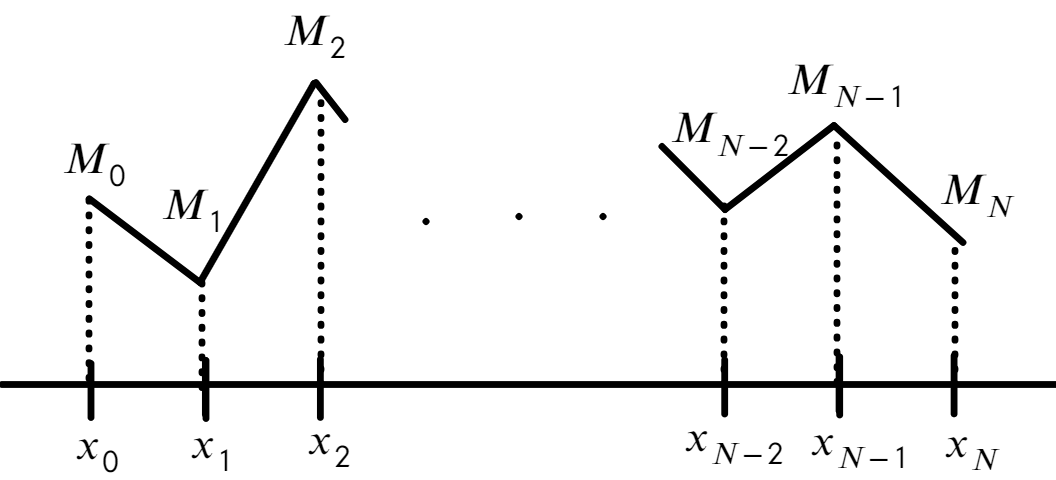
\includegraphics[scale=0.5]{img11.png}$$
	 Далее проинтегрируем соотношение (44) дважды. Опуская промежуточные выкладки, запишем формулы $$S_3'(x) = - M_{i-1}\dfrac{(x_i-x)^2}{2h_i} + M_{i}\dfrac{(x-x_{i-1})^2}{2h_i}+ \dfrac{f_i - f_{i-1}}{h_i} - \dfrac{M_i - M_{i-1}}{6}h_i,\eqno(45)$$
	 \begin{multline*}
	 	S_3(x) = M_{i-1}\dfrac{(x_i - x)^3}{6h_i} + M_{i}\dfrac{(x-x_{i-1})^3}{6h_i} + \left(f_i - M_i\dfrac{h_i^2}{6}\right)\dfrac{x-x_{i-1}}{h_i} +\\+ \left(f_{i-1} - M_{i-1}\dfrac{h_i^2}{6}\right)\dfrac{(x_i - x)}{h_i},\quad x\in [x_{i-1}, x_i],\ i = \overline{1,N}\quad(46)
	 \end{multline*}
	 Константы мы брали в соответствии с условием (42) при $j=0$. Используем оставшиеся условия из формулы (42).
	 Возьмем условие непрерывности первой производной сплайна:
	 $$\dfrac{h_i}{6}M_{i-1} + \dfrac{h_i + h_{i+1}}{3}M_i + \dfrac{h_{i+1}}{6}M_{i+1} = \dfrac{f_{i+1} - f_i}{h_{i+1}} - \dfrac{f_i - f_{i-1}}{h_i},\quad i = \overline {1,N-1}.\eqno(47)$$
	 Нам не хватает $N+1 - (N-1) = 2$ условий для констант $M_0$ и $M_{N}$. Чаще всего различают следующие способы задания дополнительных условий:
	 \begin{enumerate}
	 	\item $$M_0 =0, M_N = 0.\eqno (48)$$
	 	\item $$M_0 = f''(a), M_N = f''(b).\eqno (49)$$
	 	\item Если известны значения функции $f(x)$, то из равенства (45) можно получить условия $$\begin{cases}
	 	2M_0 + M_1 = \dfrac{6}{h_1}\left(\dfrac{f_1-f_0}{h_1} - f'(a)\right),\\
	 	M_{N-1} + 2M_N = \dfrac{6}{h_N}\left(f'(b) - \dfrac{f_N-f_{N-1}}{h_N} \right).
	 	\end{cases}\eqno(50)$$
	 \end{enumerate}
	 $\bullet$ \textit{Условия $(48)$ называются \textbf{естественными}, а сплайн называется \textbf{естественным}.}\\\\
	 $\bullet$ \textit{Если заданы условия $(49)$, то говорят, что \textbf{у сплайна на концах заданы моменты}.}\\\\
	 $\bullet$ \textit{Если пользоваться условиями $(50)$, то говорят, что \textbf{у сплайна на концах заданы наклоны}.}\\\\
	 Легко видеть, что уравнения (47) при добавлении условий или (48), или (49), или (50) представляют собой СЛАУ с трехдиагональной матрицей относительно неизвестных $M_i$. В силу строгого диагонального доминирования система имеет единственное решение и для его определения можно использовать метод прогонки. Таким образом, интерполяционный кубический сплайн всегда может быть построен и причем единственным образом.\\\\
	 Запишем алгоритм приближения функции кубическим интерполяционным сплайном. \begin{enumerate}
	 	\item Задаются исходные данные для интерполирования: значения узлов $x_i$ и значения функции в этих узлах $f(x_i)$, $i=\overline{0,N}$. Кроме того необходимо определить граничные условия (недостающие два условия). Обычно в точках $x_0, x_N$ задаются значения $f'$ или $f''$.
	 	\item Вычисляются моменты $M_i$, $i=\overline{0,N}$ как решения системы (47), дополненные условиями или (48), или (49), или (50).
	 	\item По формуле (46) вычисляются значения функции $S_3(x)$ в любой точке $x \in [a,b]$.
	 \end{enumerate}
	 \textbf{Замечания.}\begin{enumerate}
	 	\item Погрешность интерполирования естественным кубическим сплайном на всем отрезке интерполирования может быть оценена следующей константой $$|r(x)|\leq h^4\max_{x\in [a,b]}|f^{(4)}(x)|,\eqno(51)$$ где $h$ --- это расстояние между узлами (если узлы не равноотстоящие, то берется максимальное расстояние между узлами).
	 	\item Рассмотренный способ построения сплайна называется \textbf{методом моментов построения интерполяционного кубического сплайна}. Можно использовать в качестве определяющей систему наклонов $m_i = S'_3(x_i)$ в узлах $x_i$, $i=\overline{0,N}$.
	 	\item Граничные условия можно задавать и другими способами. Это связано с конкретными задачами возникающими в приложениях. Примеры:
	 	\begin{enumerate}
	 		\item смешанные граничные условия $$S_3'(a) = f'(a),\quad S_3'(b) = f''(b);$$
	 		\item условия непрерывности функции $S_3(x)$ в точках $x_1$ и $x_{N-1}$;
	 		\item условия периодичности $$S_3'(a) = S_3'(b),\quad S_3''(a) = S_3''(b).$$
	 	\end{enumerate}
	 \end{enumerate}
	 \subsubsection{Физическая интерпретация кубического сплайна.}
	 Определим следующую механическую систему. Пусть задано на плоскости 4 точки, через которые нам необходимо провести кривую, имеющую наименьшую кривизну (то есть наиболее плавные кривые). Например, такая задача может решаться при построении дорог. Для этого берутся гибкие рейки из дерева, которые закрепляют на месте, подвешивая к ним свинцовые грузила.
	 $$
	 	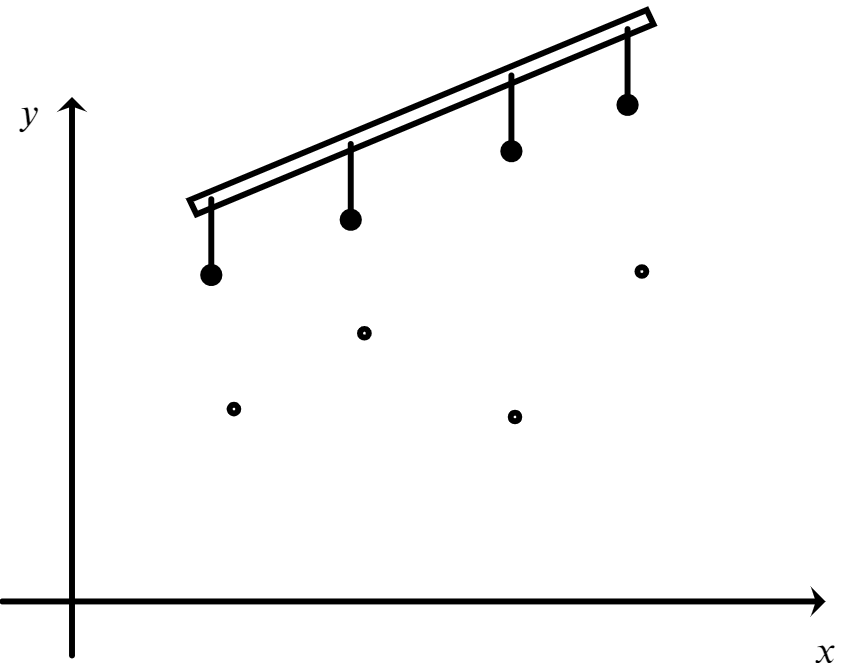
\includegraphics[scale=0.5]{img12}
	 $$
	 Изменяя положение рейки и грузил, можно добиться того, что рейка будет проходить через все точки.
	 $$
	 	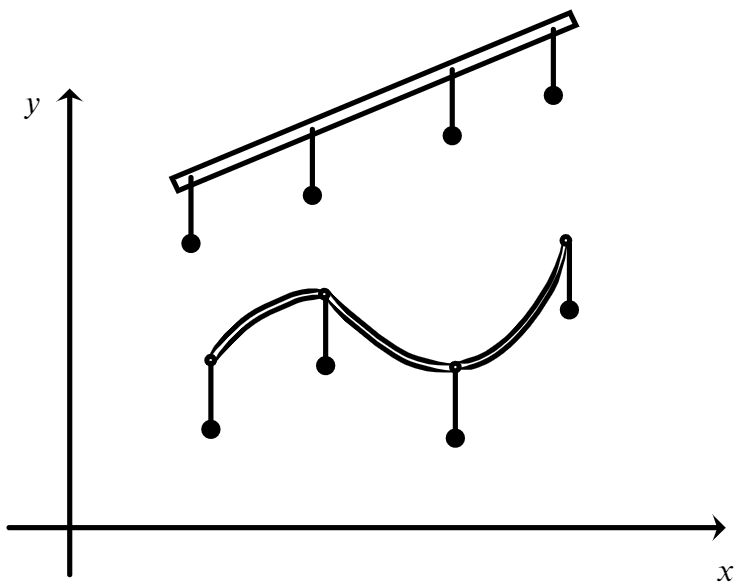
\includegraphics[scale=0.5]{img13}
	 $$
	 Если рассмотреть рейку как тонкую упругую балку, то для нее справедлив закон Бернулли-Эйлера
	 $$M(x) = EI \dfrac{1}{R(x)},$$ где $M$ --- изгибающий момент, $E$ --- модуль Юнга, $I$ --- геометрический момент инерции, $R$ --- радиус кривизны кривой $y(x)$, совпадающей с деформированной осью балки.\\\\
	 При незначительных изгибах справедливо соотношение $$R(x) \approx \dfrac{1}{y''(x)}.$$ Подставляя в уравнение для изгибающего момента, получим соотношение $$y''(x) = \dfrac{1}{EI}M(x).$$
	 При этом изгибающий момент изменяется линейно между точками закрепления грузил. Тогда очевидно, что $y(x)$ в промежутках между каждой парой соседних узлов является многочленом третьей степени. Поэтому момент --- это вторая производная, наклон --- это первая производная.\\\\
	 Если моменты на концах сплайна равны нулю, то это соответствует свободно отпущенным концам балки (рейки) и поэтому такие условия называются естественными. \\\\
	 Материальная система, являющаяся упругим бруском, проходящим через заданные точки под действием системы грузил, находится в состоянии равновесия. В этом смысле конфигурация бруска является оптимальной. Характеристикой оптимальности сплайна является кривизна линии $y(x)$. Оказывается, что интерполяционный кубический сплайн обладает минимальной кривизной среди всех интерполирующих функций.\\\\
	 $\bullet$ \textit{Свойство минимальности кривизны получило название \textbf{экстремального свойства кубического сплайна.}}\\\\
	 Рассмотрим на отрезке $[a,b]$ класс функций $W_2^2[a,b]$ --- это множество функций, имеющих интегрируемые вместе с квадратом вторые производные.\\\\
	 Поставим задачу отыскания интерполяционной функции $u(x) \in W_2^2[a,b]$, $u(x_i) = f(x_i), i=\overline{0,N}$, которая минимизирует функционал $$\Phi(u) = \int\limits_a^b (u''(x))^2dx.\eqno(52)$$
	 Если функция $u(x)$ доставляет минимум этого функционала, то эта функция будет кубическим сплайном. \\\\
	 Таким образом, мы сформулировали задачу отыскания интерполяционной функции $u(x)$, которая минимизирует функционал (52) на классе функций $W_2^2[a,b]$. Решение этой задачи дает теорема
	 \begin{theorem}
	 	Единственный минимум функционала $(52)$ достигается на кубической сплайн-функции $(46)$ с краевыми условиями $(48)$ или $(50)$.
	 \end{theorem}
	 \begin{Proof}
	 	Сперва докажем, что $$\Phi(S_3)\leq \Phi(u),\quad \forall u \in W_2^2[a,b].$$
	 	Для этого рассмотрим 
	 	\begin{multline*}
	 		\Phi(u - S_3) = \int\limits_a^b [u''(x) - S_3''(x)]^2dx = \int\limits_a^b (u''(x))^2dx - \int\limits_a^b (S''_3(x))^2dx - 2\int\limits_a^b(u''(x)-S_3''(x))S''_3(x)dx =\\ =\Phi(u) - \Phi(S_3) - 2\left[\underbrace{(u'(x) - S'_3)S''_3}_{=0}\Big|_a^b - \int\limits_a^b (u'(x) - S_3'(x))\underbrace{S'''_3(x)}_{C_i}dx\right] =\\= \Phi(u) - \Phi(S_3) +2\sum\limits_{i=1}^N C_i\int\limits_{x_{i-1}}^{x_i} (u'(x) - S'_3(x))dx = \\=\left[\text{по построению } u(x_i) =f(x_i), S_3(x_i) = f(x_i) \Rightarrow (u(x) - S_3(x))|_{x_{i-1}}^{x_i} = 0\right] =\\= \Phi(u) - \Phi(S_3).
	 	\end{multline*}
	 	Тогда $$\Phi(S_3) = \Phi(u) - \Phi(u-S_3)\leq \Phi(u).$$
	 	Мы можем утверждать, что из этого функционала $S_3$ доставляем минимум функционала. \\\\
	 	Докажем, что этот минимум единственный. Проведем доказательство от противного. Пусть кроме $S_3$ есть другая минимизирующая функция, обозначим ее $g(x)$. При этом $$\Phi(g-S_3) = 0.$$
	 	 Следовательно, $$g''(x) = S_3''(x) = 0$$ почти всюду на $[a,b]$, т.к. $g(x)$ может отличаться от $S_3$ только на линейную функцию, то есть можно представить в виде $$g(x) = S_3(x) + \alpha x + \beta.$$
	 	 Возьмем в качестве $x$ точки $x_k$, где $x_k$ --- это узлы интерполирования на $[a,b]$. Тогда $$g(x_k) = S_3(x_k) + \alpha x_k + \beta.$$
	 	 Учитывая тот факт, что $g(x_k ) = f(x_k)$, $S_3(x_k) = f(x_k)$ по построению, данное равенство возможно, если $\alpha = \beta = 0$. А значит $$g(x) = S_3(x).$$ А тогда предположение о существовании другой функции, доставляющей минимум функционала, неверное.
	 \end{Proof}
	 \section{Сходимость интерполяционного процесса.}
	 Если поставить вопрос, будет ли стремиться к нулю погрешность интерполирования $$r_n(x) = f(x) - P_n(x)\xrightarrow[n\to\infty]{}0,$$
	 то ответ, вообще говоря, будет отрицательным. Поэтому важен вопрос о поведении погрешности интерполяционного процесса.\\\\
	 Пусть функция $f(x)$ определена на отрезке $[a,b]$, а также она непрерывна на этом отрезке. Рассмотрим таблицу узлов интерполирования
	 $$X = \left( 
	 \begin{gathered} 
	 	x_0^{(0)} \hfill \\ 
	 	x_0^{(1)},\ x_1^{(1)}\hfill  \\
	 	\dots\dots\dots \hfill \\
	 	 x_0^{(n)}, x_1^{(n)},\ldots, x_n^{(n)} \hfill \\
	 	 \dots\dots\dots\dots\dots\dots \hfill
	 \end{gathered} 
	 \right)\eqno(1)$$
	 В таблице (1) все $x_i^{(k)} \in [a,b]$, $i=\overline{0,k}$ и различны для любого $k$. По каждой строке этой таблицы будем строить интерполяционный многочлен. \\\\
	 $\bullet$ \textit{Такой процесс мы будем называть \textbf{интерполяционным}.}\\\\
	 Таким образом, интерполяционный процесс задает последовательность интерполяционных многочленов $\{P_n(x)\}$, построенных по функции $f(x)$ в ее узлах $x_0^{(n)},\ldots, x_n^{(n)}$.\\\\
	 $\bullet$ \textit{Говорят, что интерполяционный процесс для функции $f(x)$ \textbf{сходится равномерно на отрезке} $[a,b]$, если выполняется условие} $$\Norm{f(x) - P_n(x)} = \max_{x\in[a,b]} |f(x) - P_n(x)|\xrightarrow[n\to\infty]{}0.\eqno(2)$$
	 Можно рассматривать и поточечную сходимость.\\\\ 
	 $\bullet$ \textit{Интерполяционный процесс \textbf{сходится в точке} $x^* \in [a,b]$, если} $$\exists \lim\limits_{n\to\infty}P_n(x^*) = f(x^*).\eqno(3)$$
	 Свойства сходимости или расходимости интерполяционного многочлена зависят как от выбора последовательности сеток $X$, так и от свойств функции $f(x)$.
	 \begin{theorem}
	 	Не существует такой таблицы узлов $X$, для которой интерполяционный процесс был бы равномерно сходящийся на отрезке $[a,b]$ для любой непрерывной функции $f(x)$.
	 \end{theorem}
	 \begin{Proof}
	 	Без доказательства.
	 \end{Proof}\\\\
	 Какова бы ни была таблица узлов, найдется непрерывная на отрезке $[a,b]$ функция $f(x)$, такая что последовательность интерполяционных многочленов не сходится к $f(x)$ равномерно.
	 Приведем примеры такой функции:
	 \begin{enumerate}
	 	\item $f(x) = |x|$, $x \in [-1,1]$. Если в качестве $X$ брать равномерную сетку узлов, то интерполяционный процесс на равномерной сетке узлов не сходится ни в одной точке отрезка, кроме узлов $-1, 0, 1$.
	 	$$
	 		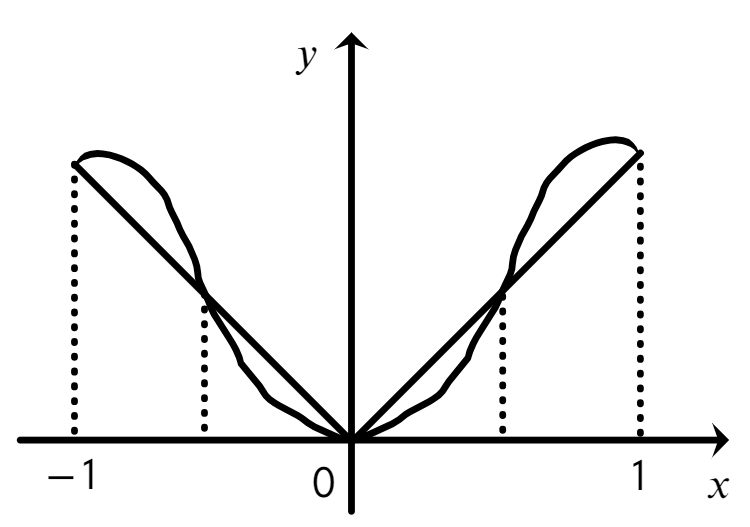
\includegraphics[scale=0.35]{img14}
	 	$$
		К примеру, удвоим количество разбиений:
		$$
			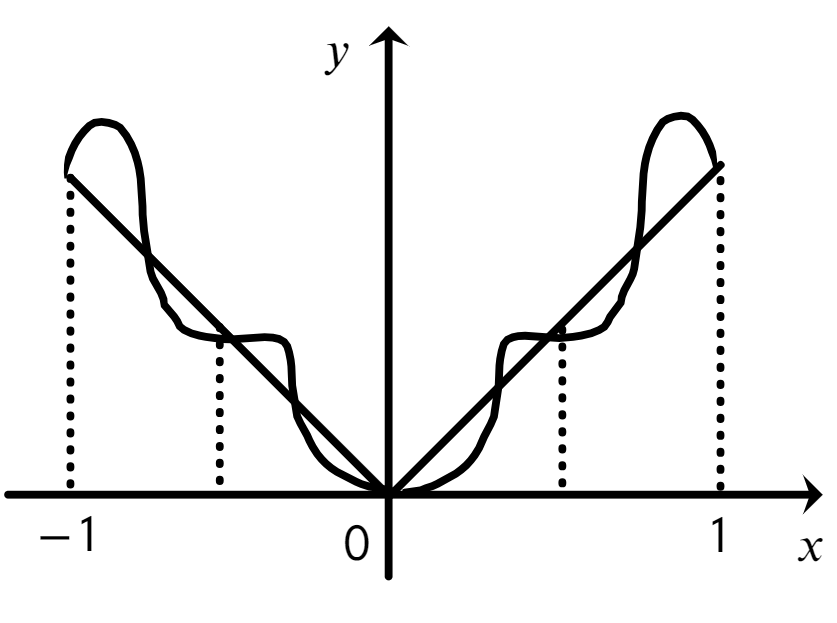
\includegraphics[scale=0.3]{img15}
		$$
		Отсюда видно, что также увеличивается и погрешность. Следовательно, максимальное расстояние между значениями полинома и значениями функции возрастает.
	 	Поэтому за исключением точек $-1, 0, 1$ интерполяционный процесс не сходится ни в одной точке.
	 	\item Функция Рунге $f(x) = \dfrac{1}{1 + 25x^2},$ $x \in [-1,1]$, для которой также интерполяционный процесс не сходится ни в одной точке.
	 \end{enumerate}
	 \begin{theorem}
	 	Для каждой непрерывной функции на отрезке $[a,b]$ существует такая таблица узлов, что соответствующий ей интерполяционный процесс сходится равномерно на этом отрезке.
	 \end{theorem}
	 \begin{Proof}
	 	Без доказательства.
	 \end{Proof}\\\\
	 Были получены результаты, которые гарантируют сходимость интерполяционного процесса.\\\\
	 $\bullet$ \textit{Функция называется \textbf{целой}, если она разложимая в степенной ряд с бесконечным радиусом сходимости.}\\\\
	 Например, если функция $f(x)$ целая, то равномерная сходимость интерполяционного процесса будет обеспечена на любой таблице узлов $X$ \\\\
	 $\bullet$ \textit{Если функция $f(x)$ представима в виде $$f(x) = \int\limits_{-1}^x \varphi(t)dt,$$ то она называется \textbf{абсолютно непрерывной}. В свою очередь функция $\varphi(t)$ должна быть абсолютно интегрируема.}\\\\
	 Если функция $f(x)$ абсолютно непрерывна на отрезке $[-1, 1]$, то равномерная сходимость возможна на сетке, построенной по корням многочленов Чебышева.\\\\
	 Но даже если интерполяционный процесс сходится, то при наличии погрешности выходных данных сам вычислительный процесс может стать неустойчивым. Поэтому интерполирование многочленом высокой степени нежелательно. По этой причине и рассматривается сплайн-интерполирование.
	 \begin{theorem}
	 	Пусть $f(x)$ является непрерывной вместе со своими производными до второго порядка включительно на отрезке $[a,b]$, то есть $f(x) \in C^2[a,b]$, и интерполирующий ее кубический сплайн определяется системой $(47)$ с условиями $(50)$. Тогда имеют место соотношения $$f^{(p)}(x) - S_3^{(p)}(x) = O(h^{2-p})\omega (h, f''),\quad p=0,1,2,\eqno(4)$$
	 	где $\omega(h,f)$ --- модуль непрерывности функции $f(x)$, то есть $$\omega (h,f) = \underset{|x_1-x_2|\leq h,\\ x_1,x_2 \in [a,b]}{\sup}|f(x_1) - f(x_2)|, \quad h = \underset{1\leq i \leq N}{\max}\{h_i\}.$$
	 \end{theorem}
	 \begin{Proof}
	 	Без доказательства.
	 \end{Proof}\\\\
	 \textbf{Замечания.}\begin{enumerate}
	 	\item Из теоремы следует равномерная сходимость при $h\to 0$ сплайна $S_3$ и его первой и второй производной к интерполируемой функции $f(x)$, а также к ее первой и второй производной, то есть $$S_3(x) \to f(x),\quad S_3'(x) \to f'(x),\quad S''_3(x)\to f''(x),\quad h\to 0.$$
	 	\item Из оценок (4) следует, что если функция $f''(x)$ удовлетворяет условию Липшица с константой $k$, то $\omega (h,f'')$ может быть оценена как $$\omega(h, f'') \leq \underset{|x_1-x_2| \leq h}{\sup} k|x_1 - x_2|\leq kh.$$
	 	Тогда $$f^{(p)}(x) - S^{(p)}_3(x) = o(h^{3-p}),\quad p=0,1,2.$$
	 	\item Если функция $f(x)\in C^4[a,b]$, то можно доказать, что $$f^{(p)}(x) - S_3^{(p)}(x) = O(h^{4-p}) \quad p=0,1,2,3$$
	 \end{enumerate}
	 Сформулируем наиболее распространенный в вычислительной практике алгоритм приближения функции с помощью интерполяционных многочленов.\\\\
	 Пусть требуется найти приближенное значение функции $f(x)$ в точке $x\in [a,b]$ с заданной точностью $\epsilon$. Для каждого значения $x$ выбирают свои узлы $x_0, x_1,\ldots, x_m$ интерполяции, ближайшие к точке $x$, и по этим узлам составляют многочлен $P_m(x)$. Тогда погрешность интерполяции в этой точке $$|r_n(x)| = |f(x) - P_m(x)| \leq \dfrac{M_{m+1}}{(m+1)!}|\omega_{m+1}(x)|,\quad M_{m+1} = \underset{\xi \in [a,b]}{\max}|f^{(m+1)} (\xi)|.$$
	 Далее для решения задачи с заданной точностью оценим $\omega_{m+1}(x)$:
	 $$\omega_{m+1}(x) = (x-x_1)\ldots (x-x_m),$$
	 этот полином ограничен равномерно по $x$, то есть $$|\omega_{m+1}(x)| < \underset{0 \leq i \leq n}{\max}|x-x_i|^{m+1}\leq (mh)^{m+1},\quad h = \underset{1 \leq i \leq m}{\max}|x_{i} - x_{i-1}|.$$
	 Таким образом, погрешность интерполяции есть величина $$|r_n(x)| = O(h^{m+1}).$$
	 Но если это так, то при фиксированной степени многочлена и уменьшении шага $h$ погрешность интерполирования неограниченно убывает. Таким образом, в случае ограниченной производной ${m+1}$-ого порядка функции $f(x)$ интерполяционный многочлен $P_m(x)$ равномерно сходится к $f(x)$ на отрезке $[a,b]$.\\\\
	 Для заданной точности $\epsilon$ определим шаг сетки из условия $$\dfrac{M_{m+1}}{(m+1)!}(mh)^{m+1}\leq \epsilon.$$
	 Тогда для всех сеток с данным и более мелким шагом и любой точки отрезка $[a,b]$ погрешность интерполяционного многочлена будет не более $\epsilon$.
	 \chapter{Численное интегрирование.}
	 \section{Постановка задачи. Основные понятия и определения.}
	 Пусть функция $f(x)$ интегрируемая по Риману на отрезке $[a,b]$. Задача заключается в отыскании значения интеграла $$I = \int\limits_a^b f(x)dx.$$
	 Аналитически эту задачу можно решить с помощью формулы Ньютона-Лейбница, а именно если можно найти для функции $f(x)$ ее первообразную $\mathcal F$, то $$I = \mathcal F(b) - \mathcal F(a).$$ Этой задачей мы заниматься не будем.\\\\
	 Вообще говоря, задача ставится таким образом, что если функция интегрируемая, а первообразной для подынтегральной функции не существует, то мы будем рассматривать вопросы, касающиеся приближенного вычисления интеграла $I$. Основной подход, который будет нами применяться, напрямую связан с заменой подынтегральной функции достаточно близкой, но более простой с точки зрения интегрирования. Например, если мы заменим функцию $f(x)$ многочленом, то мы сможем вычислить интеграл и решить задачу. Но, исходя из предыдущей главы, для хорошей замены подынтегральной функции на полином, функция должна обладать хорошими свойствами существования производных. В силу этого подынтегральную функцию чаще всего представляют в виде произведения двух. То есть в качестве задачи численного интегрирования мы будем рассматривать задачу вычисления значения $$I(f) = \int\limits_a^b p(x)f(x)dx,\eqno(1)$$ где $p(x)$ --- это фиксированная ненулевая функция, которая является весовой функцией, а $f(x)$ --- это достаточно гладкая функция, которую будем называть интегрируемой функцией. \\\\
	 Например, если нам нужно найти значение следующего интеграла, то мы можем выделить особенность функции в отдельную функцию $$\int\limits_{-1}^1 \dfrac{dx}{\sqrt{1-x^4}} = \int\limits_{-1}^1 \underbrace{\dfrac{1}{\sqrt{1-x^2}}}_{p(x)}\cdot\underbrace{\dfrac{1}{\sqrt{1+x^2}}}_{f(x)}dx.$$
	 Следуя теории интерполирования функции, интеграл $(1)$ будем вычислять следующим образом $$I (f) = \int\limits_a^b p(x) f(x)dx \approx \sum_{k=0}^{n}A_k f(x_k),\quad x_k\in[a,b],\ A_k\in \Rm.\eqno(2)$$
	 $\bullet$ \textit{При этом выражение, стоящее в правой части приближенного равенства $(2)$ называется \textbf{квадратурной суммой}, $A_k$ --- ее коэффициенты, а $x_k$ --- узлы. Само выражение $(2)$ называется \textbf{квадратурной формулой} (или квадратурное правило).}\\\\
	 При фиксированном $n$ квадратурная формула (2) зависит от $2(n+1)$ параметров $A_k, x_k$, $k=\overline{0,n}$. Выбор этих параметров осуществляется из следующих соображений.\\\\
	 Способы выбора параметров:
	 \begin{enumerate}
	 	\item \textbf{Повышение степени точности квадратурной формулы.} Сначала дадим определение термина "степень точности".\\\\
	 	$\bullet$ \textit{Квадратурная формула $(2)$ \textbf{имеет степень точности, равную $m$} относительно системы функций $\{\varphi_i(x)\}$, $i=0,1,\ldots$, если она точна для функций $\varphi_0,\ldots, \varphi_m$ и не является точной для функций $\varphi_{m+1}(x)$ и так далее. То есть выполняются соотношения} $$\begin{cases}
	 	\int\limits_a^b p(x)\varphi_i(x) dx = \sum\limits_{k=0}^{n}A_k\varphi_i(x_k),\quad i = \overline{0,m},\\
	 	\int\limits_a^b p(x)\varphi_{m+1}(x) dx\ne \sum\limits_{k=0}^{n}A_k\varphi_i(x_k).
	 	\end{cases}\eqno(3)$$
	 	Если в качестве $\{\varphi_i\}$ взять систему алгебраических многочленов $\varphi_i(x) = x^i$, то в этом случае будем иметь дело с алгебраической степенью точности. В этом случае вместо системы (3) мы получим следующее соотношение $$\begin{cases}
	 		\int\limits_a^b p(x) x^idx = \sum\limits_{k=0}^{n}A_kx^i_k,\quad i=\overline{0,m},\\
	 	\int\limits_a^b p(x) x^{m+1}dx \ne \sum\limits_{k=0}^{n}A_kx^i_k.
	 	\end{cases} \eqno(4)$$
	 	$\bullet$ \textit{Таким образом, говорят, что квадратурная формула имеет \textbf{алгебраическую степень точности $m$}.}\\\\
	 	Системы (3) и (4) можно использовать для отыскания коэффициентов квадратурной формулы.
	 	\item \textbf{Минимизация остатка на классах функций}. \\\\
	 	$\bullet$ \textit{\textbf{Остатком квадратурной формулы} $(2)$ называется величина} $$R_n(f) = \int\limits_a^b p(x)f(x)dx - \sum_{k=0}^{n}A_kf(x_k).\eqno (5)$$
	 	В формуле (5) предполагается, что $f \in F$ --- заданный класс функций. Тогда можно оценить характеристику $$\underset{f\in  F}{\sup}\ |R_n(f)|.$$
	 	В качестве условий для выбора коэффициентов $A_k$ и $x_k$ следует поставить задачу поиска минимума этой величины, то есть $$\underset{f\in F}{\sup}\ |R_n(f)|\to\min.$$
	 	В данном курсе этот подход использоваться не будет.
	 \end{enumerate}
	 \section{Интерполяционные квадратурные формулы.}
	 На отрезке интегрирования $[a,b]$ выберем $n+1$ произвольную различную точку $$x_0,x_1,\ldots, x_n \in [a,b].$$ Подынтегральную функцию $f(x)$ проинтерполируем по ее значениям в этих узлах $$f(x) = P_n(x) + r_n(x),$$ где интерполяционный многочлен запишем в форме Лагранжа $$P_n(x)=\sum_{k=0}^{n}\dfrac{\omega_{n+1}(x)}{(x-x_k)\omega_{n+1}'(x_k)}f(x_k) = \sum_{k=0}^{n} l_k(x) f(x_k),\quad l_k(x) = \dfrac{\omega_{n+1}(x)}{(x-x_k)\omega_{n+1}'(x_k)}.$$  
	 Остаток интерполяционного многочлена имеет вид $$r_n(x) = \dfrac{\omega_{n+1}(x)}{(n+1)!}f^{(n+1)}(\xi).$$
	 Тогда, пользуясь формулой для приближения функции $f(x)$, мы можем построить квадратурную формулу $$I(f) = \int\limits_a^b p(x)f(x)dx = \sum_{k=0}^{n}A_kf(x_k) + R_n(f),\eqno(1)$$
	 где коэффициенты $$A_k = \int\limits_a^b p(x) \dfrac{\omega_{n+1}(x)}{(x-x_k)\omega'_{n+1}(x_k)}dx, \eqno(2)$$
	 а величина остатка квадратурной формулы $$R_n(f) = \int\limits_a^b p(x)r_n(x)dx.\eqno(3)$$
	 Если проанализировать формулу (1), то можно заметить, что $R_n(f)$ будет достаточно малой величиной, если $r_n(x) \to 0$. Отсюда можно сделать вывод, что чем больше $n$, тем меньше будет $r_n$, а тогда $R_n(f)$ можно отбросить. И, отбрасывая остаток, мы получим приближенную формулу $$I(f) = \int\limits_a^b p(x)f(x)dx \approx \sum_{k=0}^{n}A_kf(x_k),\eqno(4)$$
	 $\bullet$ \textit{Квадратурная формула $(4)$, коэффициенты $A_k$ которой вычисляются по формуле $(2)$, называется \textbf{интерполяционной квадратурной формулой.}}\\\\
	 Установим связь между степенью точности интерполяционной квадратурной формулы и ее коэффициентами.
	 \begin{theorem}
	 	Для того, чтобы квадратурная формула $(4)$ была интерполяционной, необходимо и достаточно, чтобы она была точной для всевозможных многочленов до степени $n$ включительно.
	 \end{theorem}
	 \begin{Proof}
	 	$\Rightarrow)$ По условию формула (4) является интерполяционной. Предположим, что в этой формуле $f(x)$ --- алгебраический многочлен степени $\leq n$. Тогда при интерполировании этой функции многочленом Лагранжа очевидно, что $r_n(x) \equiv 0$. Отсюда $R_n(f) \equiv 0$, а значит квадратурная формула точна для всех многочленов степени $\leq n$.\\\\
	 	$\Leftarrow)$ Квадратурная формула точна для всех многочленов до степени $n$ включительно. Докажем, что коэффициенты вычисляются по формуле $$A_k = \int\limits_a^b p(x)l_k(x)dx,\quad k = \overline{0,n}.$$
	 	Рассмотрим интеграл $\int\limits_a^b p(x)l_k(x)dx.$
	 	Так как $l_j(x)$ является многочленом степени $n$, то для него по условию теоремы квадратурная формула будет точна, то есть $$\int\limits_a^b p(x)l_j(x)dx = \sum_{k=0}^n A_k l_j(x_k) = \left[l_j(x_k) = \delta_{kj}\right] = A_j,\quad j = \overline{0,n}.$$
	 	То есть мы показали, что если квадратурная формула точна для всех многочленов степени меньше $n$ включительно, то коэффициенты квадратурной формулы вычисляются по формуле (2).
	 \end{Proof}\\\\
	 Получим выражение для остатка квадратурной формулы. Пусть $f\in C^{n+1}[a,b]$. Тогда $$R_n(f) = \dfrac{1}{(n+1)!} \int\limits_a^b p(x)\omega_{n+1}(x)f^{(n+1)}(\xi)dx.\eqno(5)$$
	 Для того, чтобы оценить $R_n(f)$, предположим, что $$|f^{(n+1)}(x)|\leq M\quad \forall x \in [a,b].$$
	 Тогда $$|R_n(f)| \leq \dfrac{M}{(n+1)!}\cdot \int\limits_a^b |p(x)\omega_{n+1}(x)| dx.\eqno(6)$$
	 Формула (6) будет использоваться для практической оценки погрешности численного интегрирования.
	 \subsection{Формула Ньютона-Котеса.}
	 Формулы Ньютона-Котеса относятся к классу интерполяционных квадратурных формул с равноотстоящими узлами. То есть предполагается, что точки $x_k\in [a,b]$ вычисляются по формуле $$x_k = a+kh,\quad k =\overline{0,n},\quad h=\dfrac{b-a}{n}.$$
	 Точки $x_k$ мы примем за узлы квадратурной формулы, а саму формулу (4) запишем в таком виде: $$I(f) = \int\limits_a^b p(x)f(x)dx \approx (b-a)\sum_{k=0}^n B_k^n f(a+kh),\eqno(7)$$
	 где коэффициенты $$B_k^n = \dfrac{1}{b-a}A_k = \dfrac{1}{b-a}\int\limits_a^b p(x) \dfrac{\omega_{n+1}(x)}{(x-a-kh)\omega_{n+1}'(a+kh)}dx,\quad k=\overline{0,n}. \eqno(8)$$
	 Для того, чтобы оценивать эти коэффициенты, вместо (8) в вычислительной практике используется следующее выражение этих коэффициентов $$B_k^n = \dfrac{(-1)^{n-k}}{n\cdot k!(n-k)!}\int\limits_0^n p(a+th)\dfrac{t(t-1)\ldots (t-n)}{t-k}dt,\quad k=\overline{0,n}, \eqno(9)$$
	 где $t = \dfrac{x-a}{h}$. В общем случае, если весовая функция произвольная, трудно исследовать поведение этих коэффициентов. Поэтому принято рассматривать для более простых частных случаев. \\\\
	 Рассмотрим случай $p(x)\equiv1$, тогда формулы Ньютона-Котеса имеют следующие свойства:
	 \begin{enumerate}
	 	\item симметрия коэффициентов $B_k^n = B_{n-k}^n$;
	 	\item квадратурная формула (7) точна для любой функции $f(x)$ нечетной относительно середины отрезка: $$f\left(x-\dfrac{a+b}{2}\right) = -f\left(\dfrac{a+b}{2}-x\right);$$
	 	\item при четном значении $n$ квадратурная формула (7) обладает алгебраической степенью точности равной $n+1$;
	 	\item при $n\to\infty$ $$\sum_{k=0}^n |B_k^n| \to \infty,$$
	 	за счет этого формулы Ньютона-Котеса при больших $n$ становятся неустойчивыми, то есть они не гарантируют точности.
	 \end{enumerate}
	 Поэтому из 4-ого свойства для достижения требуемой точности приближенного значения интеграла исходный отрезок $[a,b]$ разбивается на отрезки небольшой длины, и на каждом из них применятся формула Ньютона-Котеса (7) при небольших значениях $n$. \\\\
	 $\bullet$ \textit{Получаемые таким образом квадратурные формулы называются \textbf{составными}, или \textbf{обобщенными}. Квадратурные формулы, не являющиеся составными, будем называть \textbf{простейшими} квадратурными формулами.}
	 \subsection{Примеры квадратурных формул при $p(x) \equiv 1$ и различных значениях $n$.}
	 \subsubsection{Формулы прямоугольников.}
	 Возьмем $n=0$. Тогда мы будем иметь один узел $x_0 \in [a,b]$ и в зависимости от расположения $x_0$ на отрезке $[a,b]$ мы будем различать разные формулы: формулы левых, правых и средних прямоугольников.\\\\
	 Например, для формулы левых прямоугольников $x_0 =a$, а полином будет иметь нулевую степень. Тогда подынтегральную функцию можно заменить многочленом нулевой степени $$f(x)\approx P_0(x) = f(a).$$
	 Тогда $$I(f) = \int\limits_a^b f(x)dx \approx (b-a)f(a) = I_{\text{лп}}(f).\eqno(10)$$
	 $\bullet$ \textit{Квадратурная формула $(10)$ называется \textbf{простейшей квадратурной формулой левых прямоугольников}.}\\\\
	 Геометрически это будет выглядеть следующим образом:
	 $$
	 	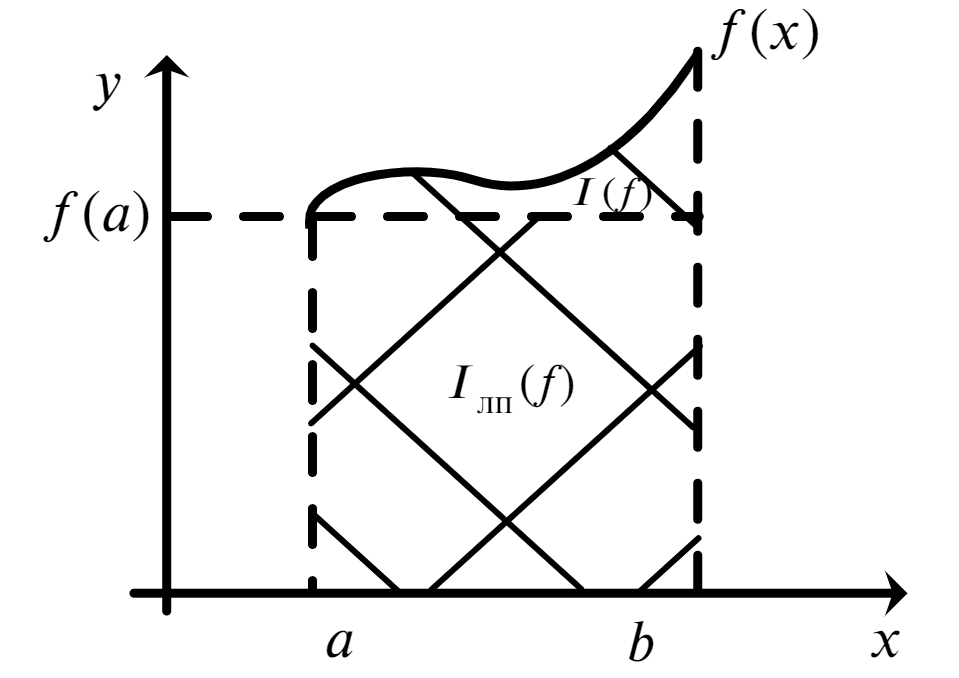
\includegraphics[scale=0.3]{img16}
	 $$
	 Если рассмотреть выражение для погрешности интерполирования, то $$r_0(x) = (x-a)f'(\xi),\quad \xi\in[a,b].$$
	 Тогда имеем формулу для оценки погрешности квадратурной формулы $$R_\text{лп}  = \int\limits_a^b r_0(x)dx = \int\limits_a^b (x-a)f'(\xi)dx.$$
	 Воспользуемся теоремой о среднем для вычисления этого интеграла. Функция на отрезке $[a,b]$ сохраняет знак, т.е. неотрицательна. Тогда по теореме о среднем существует такая точка $\eta \in [a,b]$, что $$R_\text{лп}  = \int\limits(x-a)f'(\xi)dx = f'(\eta)\int\limits_a^b(x-a)dx.$$
	 Вычислив этот интеграл, мы получим окончательную формулу $$R_\text{лп} (f) = \dfrac{(b-a)^2}{2}f'(\eta), \quad \eta \in [a,b].\eqno(11)$$ $\bullet$ \textit{Формула $(11)$ определяет \textbf{остаток простейшей квадратурной формулы левых прямоугольников}.}\\\\
	 На этом примере можно рассмотреть составные, или обобщенные, формулы левых прямоугольников. Разобьем отрезок $[a,b]$ на $N$ частей длины $$h = \dfrac{b-a}{N}.$$
	 Воспользуемся аддитивностью интеграла $$I(f) = \int\limits_a^b f(x)dx = \sum_{k=0}^{N-1}\int\limits_{x_k}^{x_{k+1}}f(x)dx,\quad x_k = a+kh,\ k = \overline{0, N}.$$
	 Для каждого этого интеграла применим формулу простейших левых прямоугольников:
	 $$I(f) =\sum_{k=0}^{N-1}\int\limits_{x_k}^{x_{k+1}}f(x)dx\approx h\sum_{k=0}^{N-1} f(x_k) = h\sum_{k=0}^{N-1} f(a+kh) = I_\text{лс}(f),\quad x_k = a+kh,\ k = \overline{0, N}.\eqno(12)$$
	 $\bullet$ \textit{Формула $(12)$ называется \textbf{составной, или обобщенной, квадратурной формулой левых прямоугольников}.}\\\\
	 У нас возникает возможность оценить погрешность, используя формулу (11), $$R_\text{лс}(f) = \dfrac{h^2}{2}\sum_{k=0}^{N-1}f'(\xi_k),\quad \xi_k \in [x_k, x_{k+1}].$$
	 Для практического использования получим более простую формулу. Предположим, что на отрезке интегрирования $f'(x)\in C[a,b]$. При этом предположении согласно теоремы Вейерштрасса на промежутке $[a,b]$ функция $f'$ достигает своих минимального и максимального значений $$m = \underset{x\in[a,b]}{\min}f'(x),\quad M = \underset{x\in[a,b]}{\max}f'(x).$$
	 В силу этого мы можем получить следующие оценки $$Nm \leq \sum_{k=0}^{N-1}f'(\xi_k)\leq NM.$$
	 Разделим на $N$, тогда $$m\leq \dfrac{1}{N}\sum_{k=0}^{N-1}f'(\xi_k)\leq M.$$
	 По теореме о промежуточном значении непрерывной функции $\exists \eta \in [a,b]$, в которой $$f'(\eta) = \dfrac{1}{N}\sum_{k=0}^{N-1}f'(\xi_k).$$
	 Используя это равенство, преобразуем выражение для остатка $$R_\text{лс}(f) = \dfrac{h^2}{2}N f'(\eta) = \dfrac{(b-a)^2}{2N}f'(\eta),\quad \eta \in [a,b].\eqno(13)$$
	 $\bullet$ \textit{Формула $(13)$ определяет \textbf{остаток составной квадратурной формулы левых прямоугольников.}}\\\\
	 В данном случае легко видеть, что $$R_\text{лс} \xrightarrow[N\to \infty]{}0.$$
	 Точки, на которые мы разбиваем отрезок, могут быть, вообще говоря, неравномерными. Но тогда все эти рассуждения станут невозможными. Поэтому эти формулы получены в предположении, что отрезок интегрирования разбивается равномерно.\\\\
	 Следуя всем ранним рассуждениям, мы можем записать квадратурную формулу правых прямоугольников:
	 $$
	 	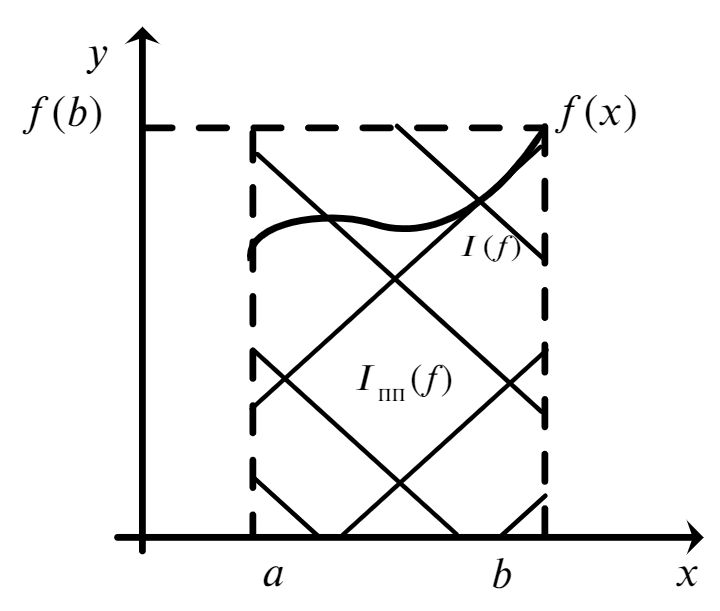
\includegraphics[scale=0.3]{img17}
	 $$
	 $$I_\text{пп}(f) = (b-a)f(b),\eqno(14)$$
	 $\bullet$ \textit{Формула $(14)$ называется \textbf{простейшей квадратурной формулой правых прямоугольников}.}
	 $$R_\text{пп}(f) = -\dfrac{(b-a)^2}{2}f'(\eta),\quad \eta\in [a,b].\eqno(15)$$
	 $\bullet$ \textit{Формула $(15)$ определяет \textbf{остаток простейшей квадратурной формулы правых прямоугольников}.}\\\\
	 По аналогии с левыми прямоугольниками запишем квадратурную составную формулу правых прямоугольников и выражение для остатка:
	 $$I_\text{пс}(f) = h\sum_{k=0}^{N-1}f(x_{k+1}) = h\sum_{k=0}^{N-1}f(a+(k+1)h),\eqno(16)$$
	 $\bullet$ \textit{Формула $(16)$ называется \textbf{составной квадратурной формулой правых прямоугольников}.}
	 $$R_\text{пс}(f) = -h\dfrac{(b-a)}{2}f'(\eta) = -\dfrac{(b-a)^2}{2N}f'(\eta).\eqno(17)$$
	 $\bullet$ \textit{Формула $(17)$ определяет \textbf{остаток составной квадратурной формулы правых прямоугольников}.}\\\\
	 Видно, что формулы остатков для левых и правых прямоугольников отличаются только знаком.\\\\
	 Тогда среднюю характеристику приближенного значения можно записать $$I\approx \dfrac12(I_\text{л} + I_\text{п}),$$
	 но точного значения мы не получим, значение будет иметь некоторую погрешность. Причем в случае составных прямоугольников погрешность будет значительно меньше.\\\\
	 Рассмотрим квадратурную формулу средних прямоугольников. Для этого возьмем узел $$x_0 = \dfrac{a+b}{2}.$$
	 Строится формула аналогичным образом: $$I_\text{сп}(f) = (b-a)f\left(\dfrac{a+b}{2}\right).\eqno(18)$$
	 $\bullet$ \textit{Формула $(18)$ называется \textbf{простейшей квадратурной формулой средних прямоугольников}.}\\\\
	 Так как точка --- это середина отрезка интегрирования, то в силу свойства 3 интерполяционных квадратурных формул Ньютона-Котеса, ее алгебраическая степень точности повышается на единицу. При этом кратность узла $x_0$ равна 2, то есть этот узел не является простым. При этом остаток соответствующей формулы Эрмита $$r_0(x) = \left(x-\dfrac{a+b}{2}\right)^2 \dfrac{f''(\xi)}{2}.$$
	 Это выражение используется для вывода формулы остатка средних прямоугольников в простейшем случае $$R_\text{сп}(f)= \int\limits_a^b \left(x-\dfrac{a+b}{2}\right)f''(\xi)dx = \dfrac{(b-a)^3}{24}f''(\eta) ,\quad \eta \in [a,b].\eqno(19)$$
	 $\bullet$ \textit{Формула $(19)$ определяет \textbf{остаток простейшей квадратурной формулы средних прямоугольников}.}\\\\
	 Запишем составные формулы средних прямоугольников:
	 $$I_\text{сс}(f) = h\sum_{k=0}^{N-1}f\left(\dfrac{x_k+x_{k+1}}{2}\right) = h\sum_{k=0}^{N-1}f\left(a+\left(k+\dfrac12\right)h\right).\eqno(20)$$
	 $\bullet$ \textit{Формула $(20)$ называется \textbf{составной квадратурной формулой средних прямоугольников}.}
	 $$R_\text{сс}(f) = h^2\cdot \dfrac{b-a}{24} f''(\eta) = \dfrac{(b-a)^3}{24N^2}f''(\eta),\quad \eta \in [a,b].\eqno(21)$$
	 $\bullet$ \textit{Формула $(21)$ определяет \textbf{остаток составной квадратурной формулы средних прямоугольников}.}\\\\
	 Формула средних прямоугольников имеет более высокую точность, чем формулы левых и правых прямоугольников.\\\\
	 Рассмотрим еще две формулы, использующие два узла.
	 \subsubsection{Квадратурная формула трапеции.}
	 В этом случае $n=1$, а в качестве узлов мы будем брать две точки $$x_0=a,\quad x_1 = b.$$
	 По этим узлам и по значениям функции в этих точках мы можем построить по определению простейшую формулу трапеций $$I_\text{тп} (f)= \dfrac{b-a}{2}\left(f(a) + f(b)\right).\eqno(22)$$
	 $\bullet$ \textit{Формула $(22)$ называется \textbf{простейшей квадратурной формулой трапеций}.}\\\\
	 Легко видеть, что формула трапеций является полусуммой значений формул по левым и по правым прямоугольникам.\\\\
	 Остаток интерполирования будет $$r_1(x) = (x-a)(x-b)\dfrac{f''(\xi)}{2}.$$
	 Подставляя в выражение для погрешности, получаем выражение для остатка формулы трапеций $$R_\text{тп}(f) = -\dfrac{(b-a)^3}{12}f''(\eta).\eqno(23)$$
	 $\bullet$ \textit{Формула $(23)$ определяет \textbf{остаток простейшей квадратурной формулы трапеций}.}\\\\
	 Если мы будем рассматривать составную формулу трапеций, то исходя из выражений выше, получим формулу $$I_\text{тс}(f) = \dfrac{h}{2}\sum_{k=0}^{N-1}(f(x_k) + f(x_{k+1})) = h\left[\dfrac{f(a)+f(b)}{2} + \sum_{k=0}^{N-1}f(x_k)\right].\eqno(24)$$
	 $\bullet$ \textit{Формула $(24)$ называется \textbf{составной квадратурной формулой трапеций}.}\\\\
	 Выражение для остатка тогда примет вид $$R_\text{тс}(f) = -h^2\dfrac{b-a}{12}f''(\eta) = -\dfrac{(b-a)^3}{12N^2}f''(\eta),\quad \eta \in [a,b].\eqno(25)$$
	 $\bullet$ \textit{Формула $(25)$ определяет \textbf{остаток составной квадратурной формулы трапеций}.}\\\\
	 Графически это можно представить в следующем виде:
	 $$
	 	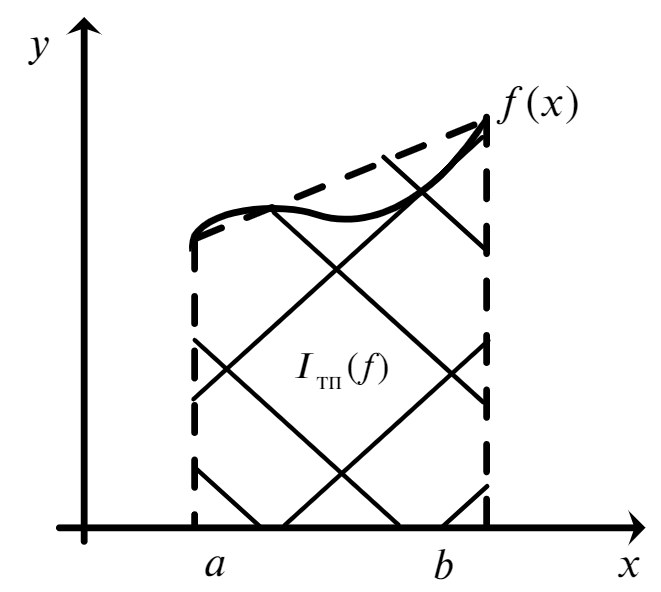
\includegraphics[scale=0.3]{img18}
	 $$
	 \subsubsection{Квадратурная формула Симпсона (парабол).}
	 В этом случае $n=2$, а узлы выбираются как $$x_0 = a,\quad x_1 = \dfrac{a+b}{2},\quad x_2 = b.$$
	 Для построения этой формулы найдем коэффициенты формулы Симпсона по выражениям (9).
	 $$B_0^2 = \dfrac{(-1)^{2-0}}{2\cdot 0!\cdot 2!}\int\limits_0^2\dfrac{t(t-1)(t-2)}{t}dt = \dfrac16 = B_2^2;$$
	 $$B_1^2 = \dfrac{(-1)^{2-1}}{2\cdot 1!\cdot 1!}\int\limits_0^2\dfrac{t(t-1)(t-2)}{(t-1)}dt =\dfrac46.$$
	 Тогда простейшая формула Симпсона имеет вид $$I_\text{симп п}(f) = \dfrac{b-a}{6}\left(f(a) + 4f\left(\dfrac{a+b}{2}\right) + f(b)\right).\eqno(26)$$
	 $\bullet$ \textit{Формула $(26)$ называется \textbf{простейшей квадратурной формула Симпсона}}.\\\\
	 Не забывая тот факт, что средняя точка увеличивает алгебраическую степень точности, то алгебраическая степень точности в данном случае будет равна 3. Также точка $x_1$ является кратным узлом. Тогда остаток многочлена Эрмита с учетом кратности среднего узла $$r_3(x) = (x-a)\left(x-\dfrac{a+b}{2}\right)^2(x-b)\dfrac{f^{(4)}(\xi)}{4!}.$$
	 Тогда $$R_\text{симп п}(f) = -\left(\dfrac{b-a}{2}\right)^5\cdot \dfrac{f^{(4)}(\eta)}{90} = -\dfrac{(b-a)^5}{2880}f^{(4)}(\eta),\quad \eta\in [a,b].\eqno(27)$$
	 $\bullet$ \textit{Формула $(27)$ определяет \textbf{остаток простейшей квадратурной формулы Симпсона}.}\\\\
	 Предполагая, что $N$ четное, будем рассматривать сдвоенный частичный отрезок $[a+(k-1)h,\ a+(k+1)h].$ Тогда формула, примененная на этом отрезке, даст в результате $$\int\limits_{a+(k-1)h}^{a+(k+1)h}f(x)\approx \dfrac h3(f(x_{k-1}) + 4f(x_k) + f(x_{k+1})),\quad k=\overline{0, N/2}.$$
	 В итоге, суммируя по всем частичным отрезкам, получим формулу составную Симпсона $$I_\text{симп с}(f) = \dfrac{h}{3}\big(f_0 + f_N + 2(f_2 + f_4 + \ldots + f_{N-2}) + 4(f_1 + f_3 + \ldots + f_{N-1})\big),\quad f_i = f(x_i).\eqno(28)$$
	 $\bullet$ \textit{Формула $(28)$ называется \textbf{составной квадратурной формулой Симпсона}.}\\\\
	 Остаток для этой формулы примет вид $$R_\text{симп с}(f) = -h^4\dfrac{b-a}{18}f^{(4)}(\eta) = -\dfrac{(b-a)^5}{180N^4}f^{(4)}(\eta),\quad \eta\in [a,b].\eqno(29)$$
	$\bullet$ \textit{Формула $(29)$ определяет \textbf{остаток составной квадратурной формулы Сипмсона}.}\\\\
	 \section{Оценка погрешности квадратурной формулы. Правило Рунге.}
	 Полученное выражение для погрешности квадратурных формул позволяет решить задачу об априорной оценке точности полученного результата. В случае составных квадратурных формул можно указать такое число разбиений $N$ (или величину шага $h = \dfrac{b-a}{N}$), при котором погрешность квадратурной формулы будет меньше заданного числа $\epsilon$, то есть $|R|\leq \epsilon$.\\\\
	 Например, для составных формул левых и правых прямоугольников мы можем оценить погрешность $$|R_\text{л(п)с}(f)|\leq \dfrac{(b-a)^2}{2N}M_1,\quad M_1 = \underset{x\in[a,b]}{\max}|f'(x)|.$$
	 Требуя, что $|R|\leq \epsilon$, мы можем получить априорную оценку количества разбиений необходимых для получения заданной точности:
	 $$N_\text{л(п)с}\geq \dfrac{(b-a)^2}{2\epsilon}\cdot M_1\quad \left(h\leq \dfrac{2\epsilon}{(b-a)M_1}\right).\eqno(30)$$
	 $$N_\text{с} \geq \sqrt{\dfrac{(b-a)^3}{24\epsilon}M_2},\quad M_2 = \underset{x\in[a,b]}{\max}|f''(x)|.\eqno(31)$$
	 $$N_\text{т} \geq \sqrt{\dfrac{(b-a)^3}{12\epsilon}M_2}.\eqno(32)$$
	 $$N_\text{симп} \geq \sqrt[4]{\dfrac{(b-a)^5}{2880\epsilon}M_4},\quad M_4 = \underset{x\in[a,b]}{\max}|f^{(4)}(x)|.\eqno(33)$$
	 Формулы (30), (31), (32), (33) считаются формулами априорной оценки погрешности численного интегрирования.
	 На практике чаще используется апостериорная оценка погрешности численного интегрирования, которая получила называние правила Рунге.\\\\
	 Пусть имеет место разложение остатка составной квадратурной формулы $$R(h,f) = c h^m + o(h^{m+1}),\quad c = \operatorname{const}.$$
	 Обозначим точное значение интеграла через $I$, а через $I_h$ --- приближенное значение соответствующее составной квадратурной формуле с шагом $h$. По предположению $$I = I_h + ch^m + O(h^{m+1})\approx I_h + ch^m.$$
	 Применим составную квадратурную формулу при разных параметрах: возьмем два значения $h_1$ и $h_2$ и найдем $I_{h_1}, I_{h_2}$. Тогда $$\begin{cases}
	 	I\approx I_{h_1} + c\cdot h_1^m,\\
	 	I\approx I_{h_2} + c\cdot h_2^m.
	 \end{cases}$$
	 Отсюда легко увидеть, что $$c\approx \dfrac{I_{h_2} - I_{h_1}}{h_1^m - h_2^m}.$$
	 Тогда подставим это $c$ в формулу для разложения остатка и получим главную часть погрешности равную $$R(h,f)\approx \dfrac{I_{h_2}-I_{h_1}}{h_1^m - h_2^m}h_1^m = \dfrac{I_{h_2}-I_{h_1}}{1 - \left(\frac{h_2}{h_1}\right)^m}.\eqno(34)$$
	 Формула (34) дает выражение для главной части остатка квадратурной формулы. Таким образом, мы можем указать алгоритм апостериорной оценки. Мы подбираем шаги $h_1$ и $h_2$ таким образом, чтобы $$|R(h,f)|\leq \epsilon,$$ тогда интеграл будет считаться вычисленным с заданной точностью.\\\\
	 \textbf{Замечания.}
	 \begin{enumerate}
	 	\item Вычисленная величина главной части остатка (34) позволяет уточнить приближенное значение интеграла $$I\approx I_{h_1} + \dfrac{I_{h_2}-I_{h_1}}{1 - \left(\frac{h_2}{h_1}\right)^m}.\eqno(35)$$
	 	Таким образом, мы повысим точность.
	 	\item При проведении расчетов обычно вычисляются интегралы с выбранным шагом $h_1$ и шагом $h_2 = \dfrac{h_1}2$. Такой способ задания изменения параметров позволяет учесть уже сделанные вычисления и таким образом оптимизировать процесс вычисления интеграла с точки зрения арифметических операций.
	 	\item Правило Рунге может быть использовано и в том случае, когда $m$ не задано.
	 \end{enumerate}
	 \section{Квадратурные формулы наивысшей алгебраической степени точности.}
	 \subsection{Основные теоремы.}
	 \begin{theorem}
	 	Для того, чтобы квадратурная формула вида $$I(f) = \int\limits_a^b p(x)f(x)dx \approx \sum_{k=0}^n A_kf(x_k)\eqno(1)$$
	 	была точной для всевозможных алгебраических многочленов до степени $(2n+1)$ включительно, необходимо и достаточно выполнение условий:
	 	\begin{enumerate}
	 		\item квадратурная формула должна быть интерполяционной, то есть $$A_k = \int\limits_a^bp(x)\dfrac{\omega_{n+1}(x)}{(x-x_k)\omega'_{n+1}(x)}dx,\quad k=\overline{0,n};\eqno(2)$$
	 		\item многочлен $\omega_{n+1}(x) = (x-x_0)\ldots (x-x_n)$ должен быть ортогональным по весу $p(x)$ на отрезке $[a,b]$ ко всем многочленам $Q_m(x)$ степеней не выше $n\geq m$, то есть $$\int\limits_a^b p(x)\omega_{n+1}(x)Q_m(x)dx = 0,\quad m=0,1,\ldots,n.\eqno(3)$$ 
	 	\end{enumerate}
	 		 \end{theorem}
	 	\begin{Proof}
	 		$\Rightarrow)$ \begin{enumerate}
	 			\item Так как квадратурная формула (1) точна для всех многочленов степени $\leq (2n+1)$, то она точна и для многочленов степени $n$ включительно. Тогда по теореме 1 из параграфа 2 квадратурная формула (1) является интерполяционной, а следовательно ее коэффициенты вычисляются по формуле (2).
	 			\item Рассмотрим произвольный многочлен $Q_m(x)$ степени $m\leq n$. Тогда степень многочлена $\omega_{n+1}(x)Q_m(x)$ будет $\leq2n+1$. Причем для любого такого полинома $$\int\limits_a^bp(x)\omega_{n+1}(x)Q_m(x)dx = \sum_{k=0}^n A_k\omega_{n+1}(x_k)Q_m(x_k) = 0.$$
	 		\end{enumerate}
	 		$\Leftarrow)$ Рассмотрим в качестве $f(x)$ произвольный алгебраический многочлен степени $\leq 2n+1$. Докажем, что для такой функции $f(x)$ формула (1) точна при выполнении условий 1 и 2. \\\\
	 		Рассмотрим отношение $\dfrac{f(x)}{\omega_{n+1}}$. По правилу деления полиномов мы можем получить $$f(x) = Q_m(x) \omega_{n+1}(x) + r(x),$$
	 		где $r(x)$ --- это остаток от деления. При этом степень частного полинома $Q_m(x)$ и степень остатка $r(x)$ не превосходит $n$. Далее рассмотрим значения функции в узлах квадратурной формулы $$f(x_k) = r(x_k),\quad k =\overline{0,n}.$$
	 		Учитывая это, вычислим исходный интеграл $$\int\limits_a^b p(x)f(x)dx = \int\limits_a^b p(x)Q_m(x)\omega_{n+1}(x)dx + \int\limits_a^b p(x) r(x) dx = \sum_{k=0}^{n}A_k r(x_k) = \sum_{k=0}^n A_kf(x_k).$$
	 		По формуле (3) первый интеграл равен нулю. Поскольку $A_k$ вычисляется по формуле (2), то эта формула является точной для всех полиномов степени $(2n+1)$ включительно.
	 	\end{Proof}
	 	\\\\
	 	Мы доказали условие, при котором достигается наивысшая степень точности. Необходимо убедиться в том, существует ли такой полином $\omega_{n+1}(x)$, который будет являться ортогональным для полиномов $Q_m(x)$.
	 	\begin{theorem}
	 		Если весовая функция $p(x)$ сохраняет знак на отрезке $[a,b]$, то многочлен $\omega_{n+1}(x)$ ортогональный по весу $p(x)$ многочленам степени $m$ существует, единственен для любого фиксированного значения $n$. При этом все его корни действительны, различны и лежат внутри отрезка $[a,b]$	 	\end{theorem}
	\begin{Proof}
		Запишем $\omega_{n+1}$ в виде многочлена с неопределенным коэффициентами: $$\omega_{n+1}(x) = x^{n+1} + a_0x^n + a_1x^{n-1} + \ldots + a_{n-1}x+a_n.$$
		Мы должны найти эти коэффициенты и определить их таким образом, чтобы выполнялось условие (3). Нахождение многочлена $\omega_{n+1}(x)$ эквивалентно нахождению его коэффициентов $a_i$, $i=\overline{0,n}$. Для определения коэффициентов $a_i$ воспользуемся условием 2 теоремы 1:
		$$\int\limits_a^b p(x)(x^{n+1} + a_0x^n + \ldots + a_{n-1}x+a_n) x^k dx= 0,\quad k=0,\ldots,n.$$
		Для однозначной разрешимости этой системы достаточно показать, что соответствующая ей однородная однозначно разрешима:
		$$\int\limits_a^b p(x)(a_0x^n + \ldots +a_n) x^k dx= 0,\quad k=\overline{0,n}.$$
		Если мы докажем, что у этой системы имеется лишь тривиальное решение $a_i = 0$, $i=\overline{0,n}$, то тем самым мы докажем существование и единственность предыдущей системы. Умножим $k$-ое уравнение этой системы на коэффициент $a_{n-k}$ и просуммируем получившееся равенство по всем $k=0,\ldots,n$. Тогда получим $$\int\limits_a^b p(x) (a_0x^n + a_1x^{n-1} + \ldots + a_n)^2dx = 0.$$
		Отсюда в силу того, что $p(x)$ сохраняет знак на $[a,b]$, то $p(x)\ne 0$ и выполнение равенства возможно тогда и только тогда, когда все коэффициенты $a_i =0$, $i=\overline{0,n}$. Таким образом, мы доказали, что многочлен $\omega_{n+1}$ всегда может быть построен, причем единственным образом.\\\\
		Рассмотрим корни многочлена $\omega_{n+1}(x)$. Пусть $\xi_1,\xi_2,\ldots,\xi_m$ --- это корни нечетной кратности, лежащие внутри отрезка $[a,b]$. Существование хотя бы одного такого корня следует из ортогональности многочлена $\omega_{n+1}(x)$ к многочлену нулевой степени. Например, $Q_0(x) \equiv 1$, тогда $$\int\limits_a^b p(x)\omega_{n+1}(x)dx = 0.$$
		Так как $p(x)$  сохраняет знак, то $\omega_{n+1}(x)$ обязано поменять знак, чтобы выполнялось равенство. Далее покажем, что таких корней будет $n+1$ штук. Рассмотрим случай, когда $1 \leq m \leq n+1$. Если рассматривается ситуация, $m < n+1$, то в этом случае мы можем построить полином $$Q_m(x)=(x-\xi_1)\ldots (x-\xi_m)$$ степени $<n+1$. Причем необходимо, чтобы $$\int\limits_a^b p(x)\omega_{n+1}Q_m(x)dx = 0.$$ Но данное равенство невозможно в силу того, что $\omega$ и $Q$ имеют одни и те же точки перемены знака. Таким образом, подынтегральное выражение сохраняет знак на $[a,b]$. Отсюда делаем вывод, что $m = n+1$.
	\end{Proof}\\\\
	Осталось доказать, что данная алгебраическая степень точности $(2n+1)$ является максимально возможной, то есть наивысшей.
	\begin{theorem}
		Если функция $p(x)$ знакопостоянна на отрезке $[a,b]$, то ни при каком выборе узлов и коэффициентов квадратурной формулы (1) не может быть точной для любого многочлена степени $2n+2$.	
	\end{theorem}
	\begin{Proof}
		Возведем в квадрат многочлен $\omega_{n+1}$. Тогда его степень станет равна $2n+2$. Рассмотрим интеграл $$\int\limits_a^b p(x)\omega_{n+1}^2(x)dx \ne 0.$$
		Его значение не обращается в ноль ни при каком выборе $x_k$, так как $\omega_{n+1}^2(x)$ не меняет знак на отрезке $[a,b]$.\\\\
		С другой стороны в приближенном равенстве (1) рассмотрим квадратурную формулу с узлами $x_k$: $$\sum_{k=0}^n A_k\omega_{n+1}^2(x_k) = 0.$$
		Что является противоречием, так как ни при каком выборе узлов $x_k$ квадратурная формула не является точной.
	\end{Proof}
	\\\\
	Таким образом, алгебраическая степень точности является наивысшей и равна $2n+1$.\\\\
	$\bullet$ \textit{Квадратурные формулы, обладающие наивысшей алгебраической степенью точности, будем называть \textbf{квадратурными формулами типа Гаусса}.}\\\\
	\textbf{Замечания.}
	\begin{enumerate}
		\item Квадратурные формулы типа Гаусса имеют все коэффициенты одного знака, что равносильно их вычислительной устойчивости.
		\item Коэффициенты квадратурных формул можно вычислять по формуле $$A_k=\dfrac{c_{n+1}}{c_n}\cdot \dfrac{1}{Q_n(x_k)Q_{n+1}'(x_k)},\quad k=\overline{0,n}.\eqno(4)$$
		В формуле (4) $Q_i(x), i=0,1,\ldots,n$ --- это система ортонормированных по весу $p(x)$ многочленов, а $c_n$ и $c_{n+1}$ --- это коэффициенты при старших степенях у многочленов $Q_n(x)$ и $Q_{n+1}(x)$.
	\end{enumerate}
	\subsection{Погрешность квадратурных формул типа Гаусса.}
	Для вычисления остатка квадратурной формулы типа Гаусса построим для функции $f(x)$ интерполяционный многочлен Эрмита степени не выше $2n+1$ с двукратными узлами $x_0, x_1,\ldots, x_n$. Тогда $$f(x) = P_{2n+1}(x) + r_{2n+1}(x),$$
	а остаток многочлена Эрмита был ранее вычислен в виде $$r_{2n+1}(x)=\omega^2_{n+1}(x)\dfrac{f^{(2n+1)}(\xi)}{(2n+2)!},\quad \xi \in [a,b].$$
	Тогда значение искомого интеграла равно $$\int\limits_a^b p(x)f(x)dx = \int\limits_a^b p(x) P_{2n+1}(x)dx + \int\limits_a^b p(x)r_{2n+1}(x)dx = \sum_{k=0}^n A_kf(x_k)(x).$$
	Причем $$\int\limits_a^b p(x) P_{2n+1}(x)dx = \sum_{k=0}^n A_kP_{2n+1}(x_k).$$
	А поскольку в точках $x_k$ значение $r_{2n+1}$ равно нулю, то $$\int\limits_a^b p(x)f(x)dx=\sum_{k=0}^n A_kP_{2n+1}(x_k) = \sum_{k=0}^n A_kf(x_k).$$
	Погрешность квадратурной формулы типа Гаусса $$R_n(f)=\int\limits_a^b p(x) \omega^2_{n+1}(x)\dfrac{f^{(2n+2)}(\xi)}{(2n+2)!}dx = \dfrac{f^{(2n+2)}(\eta)}{(2n+2)!}\int\limits_a^b p(x) \omega^2_{n+1}(x)dx.$$
	\subsection{Примеры квадратурных формул типа Гаусса.}
	\subsubsection{Случай $p(x)\equiv 1$, $[a,b] = [-1,1]$.}
	В таком случае мы имеем $$I(f) = \int\limits_{-1}^1 f(x)dx \approx \sum_{k=0}^n A_kf(x_k).\eqno(6)$$
	$\bullet$ \textit{Формула $(6)$ называется \textbf{квадратурной формулой Гаусса}.}\\\\
	Системой многочленов ортогональных по весу $p(x) = 1$ на отрезке $[-1,1]$ является система многочленов Лежандра:
	$$P_n(x)=\dfrac{1}{2^n n!}\cdot \dfrac{d^n}{dx^n}(x^2-1)^n,\quad n=0,1,\ldots$$
	Поэтому узлами $x_k$ в формуле (6) будут являться корни многочлена Лежандра, определяемые из соотношения (7) для каждого конкретного значения $n$
	$$P_{n+1}(x) = 0.\eqno(7)$$
	А коэффициенты $A_k$, следуя формуле (4), можно представить в виде $$A_k = \dfrac{2}{(1-x_k^2) [P'_{n+1}(x_k)]^2},\quad k=\overline{0,n}.\eqno(8)$$
	Из формулы (7) ищем узлы $x_k$, по найденным $x_k$ из формулы (8) ищем коэффициенты $A_k$, а остаток при этом оценивается аналитически выражением $$R_n(f) = \dfrac{2^{2n+3}}{(2n+3)(2n+2)!}\left[\dfrac{(n+1)!^2}{(2n+2)!}\right]^2 f^{(2n+2)}(\eta).\eqno(9)$$
	\subsubsection{Случай $p(x) = \dfrac{1}{\sqrt{1-x^2}}$ $[a,b]=[-1,1]$.}
	Квадратурная формула в этом случае будет иметь вид $$I(f) = \int\limits_{-1}^1\dfrac{1}{\sqrt{1-x^2}}f(x)dx \approx \sum_{k=0}^{n}A_k f(x_k).\eqno(10)$$
	Для этой формулы системой ортогональных многочленов является система многочленов Чебышева $T_n(x)$. В качестве узлов квадратурной формулы (10) выбираются корни многочлена $T_{n+1}(x)$, то есть решается уравнение $$T_{n+1}(x) = 0.$$
	Если мы решим это уравнение, то получим корни вида $$x_k = \cos\dfrac{2k+1}{2n+2}\pi,\quad k = \overline{0,n}. \eqno(11)$$
	Причем все $A_k$ равны между собой и принимают значения $$A_k = \dfrac{\pi}{n+1},\quad k=\overline{0,n}\eqno(12)$$
	$\bullet$ \textit{Формула $(10)$ с узлами $(11)$ и коэффициентами $(12)$ и называется \textbf{квадратурной формулой Эрмита}.}\\\\
	Можно получить выражение для остатка этой формулы $$R_n(f) = \dfrac{\pi}{2^{2n+1}(2n+2)!}\cdot f^{(2n+2)}(\eta),\quad \eta\in [-1,1].\eqno(13)$$
	\textbf{Замечания.}
	\begin{enumerate}
		\item Для применения формул Гаусса и Эрмита в случае произвольного отрезка $[a,b]$ необходимо использовать линейное преобразование $$x = \dfrac{b-a}{2}x' + \dfrac{a+b}{2},\quad x' \in [-1,1].$$
		Тогда $x$ будет изменяться на отрезке $[a,b]$. Остаток квадратурной формулы для промежутка $[a,b]$ выражается через остаток на отрезке $[-1,1]$ следующим образом: $$R_n(f) = \left(\dfrac{b-a}{2}\right)^{2n+3}R_n(f).\eqno(14)$$
		\item В приложениях в зависимости от свойств интегралов и интегрируемых функций применяются специальные квадратурные формулы разработанные для таких особенностей. Перечислим некоторые наиболее часто применяемые:
		\begin{enumerate}
			\item квадратурные формулы с равными коэффициентами (квадратурные формулы Чебышева);
			\item квадратурные формулы с наперед заданными узлами (квадратурные формулы Маркова);
			\item специальные квадратурные формулы Эйлера.
		\end{enumerate}
	\end{enumerate}
	\section{Вычисление кратных интегралов.}
	\subsection{Постановка задачи и пути ее решения.}
	Пусть в $n$-мерном пространстве $E_n$ необходимо вычислить интеграл по области $\Omega$ вида $$I = \int\limits_\Omega p(x)f(x)dx,\eqno(1)$$
	где $x = (x_1,\ldots, x_n)$, $dx = dx_1\ldots dx_n$, $p(x)$ --- весовая функция, $f(x)$ --- интегрируемая функция. Как и ранее, весовая функция включает в себя все особенности подынтегрального выражения, но при этом мы должны быть уверены, что существуют интегралы $$\mu_{\alpha_1\ldots \alpha_n} = \int\limits_\Omega p(x)x_1^{\alpha_1}\ldots x_n^{\alpha_n}dx.$$
	Действуя по аналогии со случаем одномерных интегралов, приближенная формула для вычисления (1) выглядит $$I = \int\limits_\Omega p(x)f(x)dx \approx \sum_{k=0}^{K}A_kf(x^{(k)}).\eqno(2)$$
	$\bullet$ \textit{Выражение $(2)$ называется \textbf{кубатурной формулой для вычисления кратного интеграла}, $A_k$ --- коэффициенты, $x_k$ --- узлы, $k=\overline{0,K}$.}\\\\
	Выбор коэффициентов $A_k$ и узлов $x_k$ кубатурной формулы (2) будем осуществлять исходя из замены подынтегральной функции интерполяционным многочленом. А условие выбора коэффициентов $A_k$ и $x_k$ будем получать исходя из алгебраической степени точности.\\\\
	Так, если мы хотим получить наивысшую алгебраическую степень точности, то необходимо, чтобы формула была интерполяционной и распределение узлов было связано с поверхностями, определяемыми ортогональными многочленами.\\\\
	Далее будем рассматривать случай $n=2$, то есть на примере двойных интегралов.
	\subsection{Кубатурные формулы основанные на сведении кратного интеграла к повторному.}
	Если случай $n=2$, то рассмотри интеграл по плоской фигуре и в качестве $\Omega$ возьмем прямоугольник $$\Omega = \{(x,y): a\leq x \leq b, c \leq y \leq d\}.$$
	Также возьмем $p(x)\equiv 1$. Тогда интеграл (1) можно записать в виде $$\int\limits_a^b\int\limits_c^d f(x,y)dxdy = \int\limits_a^b F(x)dx,\quad F(x) = \int\limits_c^d f(x,y)dy.\eqno(3)$$
	Таким образом, процесс вычисления двойного интеграла сводится к процессу последовательного вычисления одномерных интегралов. Для одномерных интегралов можно применить теорию квадратурных формул. Поэтому построим простейшие кубатурные формулы средних прямоугольников, трапеций и Симпсона.
	\begin{enumerate}
		\item \textbf{Кубатурная формула средних прямоугольников.}
		Вычисляем $F(x)$:
		$$F(x) = \int\limits_c^d f(x,y)dy \approx (d-c)f\left(c, \dfrac{c+d}{2}\right).
		$$
		Теперь подставим вычисленное значение $$I = \int\limits_a^b (d-c)f\left(x, \dfrac{c+d}{2}\right)\approx (b-a)(d-c)f\left(\dfrac{a+b}{2}, \dfrac{c+d}{2}\right)=S f\left(\dfrac{a+b}{2}, \dfrac{c+d}{2}\right).\eqno(4)$$
		$\bullet$ \textit{Формула $(4)$ является \textbf{кубатурной формулой средних прямоугольников}.}\\\\
		\item \textbf{Кубатурная формула трапеций.}
		$$I=\int\limits_a^b \int\limits_c^d f(x,y)dxdy\approx \dfrac{S}{4}\left[f(a,c) + f(b,c)+f(a,d)+f(b,d)\right].\eqno(5)$$
		\item \textbf{Кубатурная формула Симпсона.}
		\begin{multline*}
			I=\int\limits_a^b \int\limits_c^d f(x,y)dxdy\approx \dfrac{S}{36}\left[f(a,c) + f(b,c)+f(a,d)+f(b,d)\right] +\\+ \dfrac S9 \left[f\left(a,\dfrac{c+d}{2}\right) + f\left(\dfrac{a+b}{2},c\right)+f\left(\dfrac{a+b}{2},d\right)+f\left(b,\dfrac{c+d}{2}\right) +4f\left(\dfrac{a+b}{2},\dfrac{c+d}{2}\right)\right].\quad(6)
		\end{multline*}
	\end{enumerate}
	В общем случае для построения интерполяционных кубатруных формул необходимо воспользоваться формулами повторного интерполирования. Выпишем формулу многочлена Лагранжа для двух переменных:
	$$P_{n,m}(x,y)=\sum_{i=0}^{n}\sum_{j=0}^{m}\dfrac{\omega_{n+1}(x)\omega_{m+1}(x)}{(x-x_i)(y-y_j)\omega'_{n+1}(x_i)\omega'_{n+1}(y_j)}f(x_i,y_j).$$
	Тогда $$I = \int\limits_a^bdx\int\limits_c^d f(x,y)dy \approx \sum_{i=0}^{n}\sum_{j=0}^{m} f(x_i,y_j)\int\limits_a^b \dfrac{\omega_{n+1}(x)}{(x-x_i)\omega'_{n+1}(x_i)}dx+\int\limits_c^d \dfrac{\omega_{n+1}(y)}{(y-y_j)\omega'_{n+1}(y_j)}dy.\eqno(7)$$
	\textbf{Замечания.}
	\begin{enumerate}
		\item Если область не является прямоугольником, то применяется либо разбиение ее на подобласти, либо, если это возможно, используется отображение данной области на подобную область (конформные отображения).
		\item На базе простейших формул (4)-(6) можно строить составные кубатурные формулы. Выражения для остатка кубатурных формул могут быть получены аналогично квадратурным формулам.
	\end{enumerate}
	\subsection{Кубатурные формулы, основанные на использовании определения АСТ.}
	Рассмотрим случай $\Omega = [a,b]\times [c,d]$, $p(x)\equiv1$, $K = 0$, то есть один узел. По определению алгебраической степени точности построим кубатурную формулу, точную для всех многочленов нулевой и первой степени. Для этого подставим в формулу (2) вместо $f(x,y)$ полиномы нулевой степени --- $1$, а затем первой степени --- $x,y$.
	$$\iint\limits_\Omega dx dy = (b-a)(d-c).$$
	$$\iint\limits_\Omega x dx dy = (d-c)\dfrac{b^2-a^2}{2}.$$
	$$\iint\limits_\Omega ydx dy = (b-a)\dfrac{d^2-c^2}{2}.$$
	Теперь запишем условия АСТ $$\begin{cases}
		(b-a)(c-d)= A_0,\\
		(d-c)\dfrac{b^2-a^2}{2} =A_0x_0,\\
		(b-a)\dfrac{d^2-c^2}{2}=A_0y_0.
	\end{cases}$$
	Тогда $A_0 = S$ --- площадь прямоугольника. Тогда, подставляя, получаем $$\begin{cases}
		A_0 = S,\\
		x_0 = \dfrac{a+b}{2},\\
		y_0 = \dfrac{c+d}{2}.
	\end{cases}$$
	Таким образом, мы получили кубатурную формулу, совпадающую с формулой средних прямоугольников, которая обладает алгебраической степенью точности по крайней мере 1. Причем можно убедиться, что она не больше единицы, если подставить вместо $f(x,y)$ теперь $x^2, y^2, xy$ и проверить, является ли формула точной.\\\\
	Рассмотрим остаток этой формулы. Используя разложение функции $f(x,y)$ в ряд Тейлора, мы можем получить выражение для остатка формулы средних прямоугольников:
	$$R_\text{с,п}^\text{куб} = \int\limits_a^b\int\limits_c^d f(x,y)dxdy - S f\left(\dfrac{a+b}{2}, \dfrac{c+d}{2}\right)\approx \dfrac{1}{24} S\left[(b-a)^2f''_{xx} + (d-c)^2f''_{yy}\right].\eqno(8)$$
	$\bullet$ \textit{Формула $(8)$ является \textbf{выражением для остатка простейшей кубатурной формулы средних прямоугольников}}.\\\\
	Для повышения точности можно разбить область $\Omega$ на прямоугольные ячейки:
	$$\Delta \Omega_{ij} = \left\{(x,y) : \begin{matrix}x_{i-1}\leq x \leq x_{i+1},& i= \overline{1,N}\\ y_{j-1}\leq y \leq y_{j+1},& j= \overline{1,M}\end{matrix}\right\},$$
	где $N$ и $M$ --- количество разбиений каждого из отрезков.
	$$
		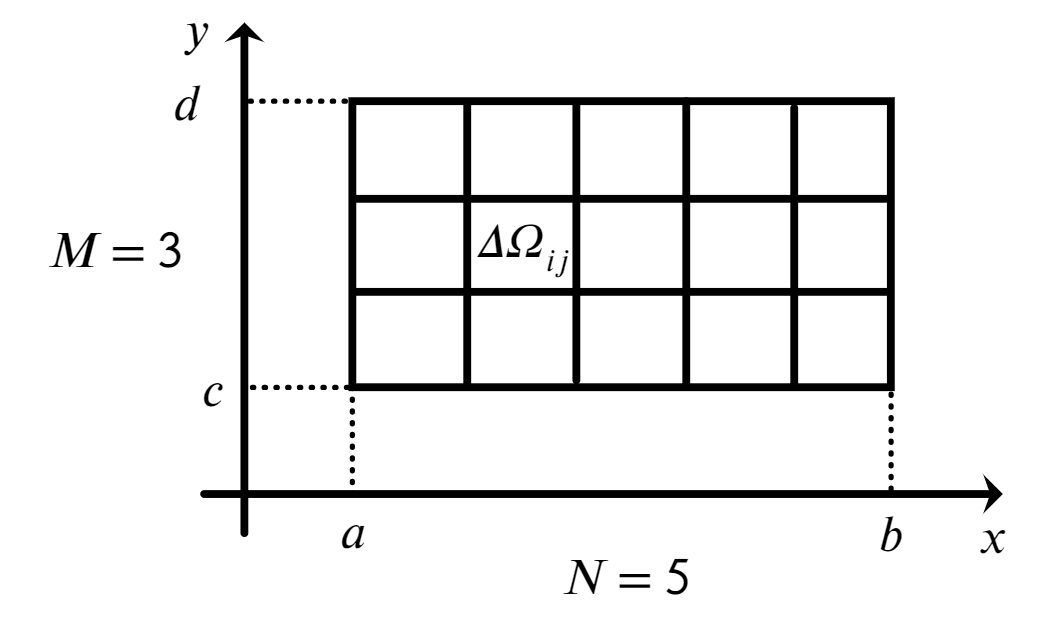
\includegraphics[scale=0.35]{img19}
	$$
	Тогда на каждом элементарном прямоугольнике $\Delta \Omega_{ij}$ мы применяем формулу средних прямоугольников:
	$$\iint\limits_{\Delta\Omega_{ij}} f(x,y)dx dy \approx \Delta x_i \cdot \Delta y_j \cdot f(\overline x_i, \overline y_j),$$
	где $$\begin{matrix}
		\Delta x_i  = x_i - x_{i-1},\\
		\Delta y_j = y_j - y_{j-1},\\
		\overline{x}_i = \dfrac{x_{i-1}+x_i}{2},\\
		\overline y_j = \dfrac{y_{j-1} + y_j}{2}.
	\end{matrix}$$
	Тогда можно записать обобщенную формулу средних прямоугольников $$\iint\limits _\Omega f(x,y)dx dy \approx \sum_{i=1}^{N}\sum_{j=0}^{M}\Delta x_i \Delta y_j f(\overline x_i, \overline y_j).\eqno(9)$$
	$\bullet$ \textit{Формула $(9)$ называется \textbf{составной кубатурной формулой средних прямоугольников.}}\\\\
	Остаток составной кубатурной формулы средних прямоугольников
	$$R_\text{с,с}^\text{куб} \approx \dfrac{1}{24}\left[\left(\dfrac{b-a}{N}\right)^2\iint\limits_\Omega f_{xx}'' d\Omega + \left(\dfrac{d-c}{M}\right)^2 \iint\limits_\Omega f_{yy}'' d\Omega\right] = O(N^{-2} + M^{-2}) = O(\Delta x^2 + \Delta y^2),\eqno(10)$$
	где $\Delta x = \underset{i}{\max} \Delta x_i$, $\Delta y = \underset{j}{\max}\Delta y_j$. \\\\
	Формула (10) говорит о том, что при $N$ и $M$, стремящимся к бесконечности приближенное значение интеграла стремится к точному.\\\\
	Для корректного применения составных кубатурных формул следует иметь ввиду, что увеличивать количество разбиений нужно одновременно, то есть $$\dfrac N M = \operatorname{const}.$$
	Формулу средних прямоугольников можно обобщить и на более сложные области. Если у нас имеется интеграл по нерегулярной области $\Omega$ $$\iint\limits_\Omega f(x,y)dxdy \approx S(\Omega) f(\overline x, \overline y),\eqno(11)$$
	где $S(\Omega)$ --- площадь области $\Omega$, а $\overline x, \overline y$ --- координаты центра тяжести этой площади. В общем случае площадь и координаты центра тяжести можно посчитать как $$S(\Omega) = \iint\limits_\Omega dxdy,\quad \overline x = \dfrac{1}{S(\Omega)}\iint\limits_\Omega x dxdy,\quad \overline y = \dfrac{1}{S(\Omega)}\iint\limits_\Omega y dxdy.$$
	$\bullet$ \textit{Формула $(11)$ называется \textbf{формулой средних}. В литературе способ получения кубатурных формул средних называется \textbf{методом ячеек}.}\\\\
	Очевидно, что у формулы (11) АСТ равна единице. При любом другом расположении узлов АСТ понижается и становится равной нулю (например, если $x \ne \overline x, y = \overline {y}$).\\\\
	При практических вычислениях часто в качестве $\Omega$ рассматривают треугольник. Пусть $\Omega$ является треугольником с вершинами $A, B, C$. Координаты вершин $(x_A, y_A), (x_B,y_B), (x_C,y_C)$ полностью определяют данный треугольник на плоскости. Тогда для того, чтобы посчитать площадь этого треугольника, введем функцию координат $$S_\Delta = \dfrac{1}{2}|g(A,B,C)|,\eqno(12)$$
	где функция координат $$g(A,B,C) = \begin{vmatrix}
		x_A & y_A & 1\\
		x_B & y_B & 1\\
		x_C & y_C & 1\\
	\end{vmatrix}.$$
	Для того, чтобы построить формулу (11) по формуле средних в случае треугольника, нам достаточно выбрать в качестве центра тяжести величину, равную точке $$\overline x = x_M = \dfrac{x_A + x_B + x_C}{3},\quad \overline {y} = y_M = \dfrac{y_A + y_B + y_C}{3}.\eqno(13)$$ Геометрически это точка пересечения медиан треугольника. \\\\
	Таким образом, используя формулы (12) и (13), можно построить формулу средних, подставив эти значения в формулу (11).\\\\
	Кроме прямоугольников и треугольников в качестве области, площадь и центр тяжести которой легко определить, можно рассматривать и другие фигуры (области), для которых легко посчитать площадь и центр тяжести, например, правильные многоугольники, окружность, трапеция (равнобедренная).\\\\
	В качестве примера построим формулу трапеций для треугольника. Имеется интеграл $$\iint\limits_\Delta f(x,y)dxdy,$$ построим для него кубатурную формулу трапеций. Заменим функцию $f(x,y)$ интерполяционным многочленом 1 степени, где узлами будут являться значения функции в вершинах треугольника. Это будет полином первой степени и будет выражаться следующим соотношением:
	$$P_1(x,y) = \dfrac{1}{g(A,C,B)}\left[f(A)g(Q,C,B) + f(B)g(A,C,Q) + f(C)g(A,Q,B)\right],$$
	где $Q(x,y)$ --- произвольная точка на плоскости с координатами $(x,y)$. Известно, что, подставляя любую точку, мы будем иметь линейный функционал. Если мы подставим вместо $f$ полином, а потом вычислим этот полином точно, то мы тем самым получим кубатурную формулу для вычисления этого интеграла. При этом мы должны гарантировать, что при подстановке мы получим точное равенство.\\\\
	Подставляем в интеграл полином, а затем применяем формулу средних \begin{multline*}
		\iint\limits_\Delta f(x,y)dxdy\approx \iint\limits_\Delta P_1(x,y)dxdy =\\= \dfrac{1}{g(A,C,B)}S_\Delta \left[f(A)g(M, C, B)+  f(B)g(A, C, M) + f(C)g(A,M,B)\right].
 	\end{multline*}
	Упростим эту формулу, учитывая, что $g(M, C, B) = \dfrac{1}{3}g(A,C,B)$, $g(A, C, M) = \dfrac{1}{3}g(A,C,B)$, $g(A, M, B) = \dfrac{1}{3}g(A,C,B)$,
	$$\iint\limits_\Delta f(x,y)dxdy \approx \dfrac{S_\Delta}{3}(f(A) + f(B) + f(C)).\eqno(14)$$
	Формула (14) и является формулой трапеций для треугольника.
	\chapter{Методы решения интегральных уравнений.}
	\section{Постановка задачи.}
	$\bullet$ \textit{\textbf{Интегральным уравнением} называется такое уравнение, неизвестная функция в котором содержится под знаком интеграла. В общем случае интегральное уравнение имеет вид} $$\int\limits_a^b \mathcal K(x,s,u(s))ds = f(x,u(x)),\quad a \leq x \leq b,\eqno(1)$$
	\textit{здесь $x$ --- независимая переменная, $u(x)$ --- искомая функция, $\mathcal K(x,s,u(s))$ --- ядро интегрального уравнения, $f$ --- правая часть уравнения, $s$ --- переменная интегрирования. }\\\\
	Мы будем рассматривать наиболее часто встречающиеся в приложениях линейные интегральные уравнения, то есть те, в которых искомая функция $u(x)$ входит как линейный множитель, имеющие вид $$\int\limits_a^b \mathcal K( x,s)u(s)ds = f(x),\quad a \leq x \leq b.\eqno(2)$$
	Если же выделяется линейное слагаемое из правой части, то можно рассматривать уравнения $$u(x) - \lambda \int\limits_a^b \mathcal K(x,s)u(s)ds = f(x),\quad a \leq x \leq b,\ \lambda \in \Rm\eqno(3)$$
	где $\lambda$ --- известная постоянная.\\\\
	$\bullet$ \textit{Уравнения $(2)$ и $(3)$ называются соответственно \textbf{интегральными уравнениями Фредгольма 1-го и 2-го рода}.}\\\\
	Кроме уравнений (2) и (3) рассматриваются также уравнения Вольтерра. \\\\
	$\bullet$ \textit{Если $\mathcal K(x,s) = 0$ при $x<s$, то уравнения $(2)$ и $(3)$ переходят в \textbf{интегральные уравнения Вольтерра 1-го и 2-го рода}:}
	$$\int\limits_a^x \mathcal K( x,s)u(s)ds = f(x),\quad a \leq x \leq b,\eqno(4)$$
	$$u(x) - \lambda \int\limits_x^b \mathcal K(x,s)u(s)ds = f(x),\quad a\leq x\leq b.\eqno(5)$$
	В дальнейшем мы будем рассматривать только интегральные уравнения 2-го рода, поскольку интегральные уравнения 1-го рода являются некорректно поставленными. \\\\
	Для однородных интегральных уравнений Фредгольма 2-го рода может быть поставлена задача на собственные значения. Сформулируем ее. \\\\
	$\bullet$ \textit{Параметры $\lambda_i$, при которых уравнение вида $$u(x) = \lambda\int\limits_a^b \mathcal K(s,x)u(s)ds,\quad a\leq x \leq b\eqno(6)$$ имеет отличные от нуля решения $u(x) = \varphi_i(x)\ne 0$, называются \textbf{собственными значениями} ядра $\mathcal K(x,s)$, или уравнения, а отвечающие им решения называются \textbf{собственными функциями}.}
	\begin{theorem}
		[Фредгольма]
		Если $\lambda$ не является собственным значением ядра $\mathcal K(x,s)$, то неоднородное уравнение $(3)$ имеет единственное непрерывное решение на отрезке $[a,b]$. В противном случае данное однородное уравнение либо не имеет решений, либо имеет их бесчисленное множество. 
	\end{theorem}
	\begin{Proof}
		Без доказательства.
	\end{Proof}\\\\
	Данная теорема дает ответ на вопрос о существовании и единственности решения интегрального уравнения Фредгольма 2-го рода.\\\\
	Решение соответствующего однородного уравнения для уравнения Вольтерра 2-го рода имеет лишь тривиальное решение $u \equiv 0$. Тогда при любых $\lambda$ неоднородное уравнение будет иметь решение, при этом единственное.\\\\
	Таким образом, для уравнений Вольтерра решение всегда существует и единственно, а для уравнений Фредгольма задача является корректно поставленной, значит решение также может быть найдено единственным образом.
	\section{Метод механических квадратур.}
	\subsection{Случай ИУФ-2.}
	Рассмотрим ИУФ-2 $$u(x) - \lambda \int\limits_a^b \mathcal K(x,s)u(s)ds = f(x),\quad a\leq x \leq b, \lambda \in \Rm.\eqno(1)$$
	На отрезке $[a,b]$ выберем $n+1$ точку $$a \leq x_0 < x_1 <\ldots < x_n \leq b$$ и заменим в формуле (1) интеграл квадратурной суммой. Причем точки $x_k$ будут являться узлами квадратурной формулы. Тогда вместо (1) мы получим новую формулу $$u(x) - \lambda \sum_{k=0}^{n}A_k \mathcal K(x,x_k)u(x_k) = f(x) + \lambda \rho(x),\quad a\leq x \leq b, \lambda \in \Rm.\eqno(2)$$
	где $A_k$ --- это коэффициенты квадратурной формулы, а $\rho(x)$ --- остаток квадратурной формулы. Например, если в качестве квадратурной формулы использовать составную квадратурную формулу средних прямоугольников, то $$x_k = a + \left(k + \dfrac12\right)h,\quad k = \overline{0,n-1},\quad h =\dfrac{b-a}{n},\quad A_k = h,$$ $$\rho(x) = \dfrac{h^2}{24}(b-a)\cdot \dfrac{\partial^2}{\partial S^2}[\mathcal K(x,\eta), u(\eta)],\eta \in [a,b].$$
	Если в (2) вместо $x$ выбирать значения $x_i$ и последовательно вычислять $u(x_i)$, то мы тогда получим систему $n+1$ уравнений
	$$u(x_i) - \lambda \sum_{k=0}^{n}A_k \mathcal K(x_i,x_k)u(x_k) = f(x_i) + \lambda \rho(x_i),\quad a\leq x \leq b,\ \lambda \in \Rm,\quad i=\overline{0,n}.\eqno(3)$$
	Принимая во внимание то, что если величина $\lambda \rho(x)$ является достаточно малой и мы можем ее отбросить, то вместо (3) получим систему $$y_i - \lambda \sum_{k=0}^{n}A_k \mathcal K_{ik}y_k = f_i\eqno(4)$$
	где $y_i \approx u(x_i)$, $\mathcal K_{ik} = \mathcal K(x_i, x_k)$, $f_i=f(x_i)$. Таким образом, решение системы (4) является приближенным значением к точному значению исходного уравнения в узлах $x_i$. Найти $y_i$ из системы (4) можно любым методом решения СЛАУ.\\\\
	Приближенное значение во всех точках отрезка можно найти по формуле $$y(x) = f(x) + \lambda \sum_{k=0}^n A_k\mathcal K (x, x_k)y_k,\quad x\in [a,b].\eqno(5)$$
	Таким образом, алгоритм метода механических квадратур для решения ИУФ-2 таков:
	\begin{enumerate}
		\item Задаем количество разбиений отрезка $n$, узлы $x_k$ и выбираем соответствующую квадратурную формулу, которая определяется коэффициентами $A_k$.
		\item Составляем СЛАУ вида $Ay = f$, где $A$ --- матрица размерности $n+1\times n+1$
		$$A = \begin{pmatrix}
			1 - \lambda A_0 \mathcal K_{00} & -\lambda A_1 \mathcal K_{01} & \ldots & -\lambda A_n \mathcal K_{0n}\\
			\vdots & \vdots & \ddots & \vdots \\
			 - \lambda A_0 \mathcal K_{n0} & -\lambda A_1 \mathcal K_{n1} & \ldots & 1-\lambda A_n \mathcal K_{nn}\\
		\end{pmatrix},\quad f= \begin{pmatrix}
		f_0 \\ \vdots \\ f_n
		\end{pmatrix}$$
		\item Решаем систему выбранным методом (например, методом Гаусса).
		\item Восстанавливаем решение в любых точках отрезка, вычисляя $y(x)$ $\forall x \in [a,b]$ по формуле (5).
 	\end{enumerate}
 	\textbf{Замечания.}
 	\begin{enumerate}
 		\item Для восстановления решения кроме формулы (5) можно использовать теорию интерполирования.
 		\item Если $\lambda$ будет являться собственным значением уравнения, то определитель матрицы $A$ может стать равен нулю. Но в этом случае получается задача на собственные значения. Занулив правую часть, мы можем найти собственные функции ядра, решая однородную систему.
 		\item Для уточнения результата по правилу Рунге можно произвести расчеты на вложенных сетках, имеющих не пустое пересечение множества узлов.
 	\end{enumerate}
 	\subsection{Случай ИУВ-2.}
 	Рассмотрим ИУВ-2 $$u(x) - \lambda \int\limits_a^x \mathcal K(x,s)u(s)ds = f(x),\quad a\leq x \leq b,\ \lambda \in \Rm.\eqno(6)$$
 	На отрезке $[a,b]$ выберем $n+1$ точку $$a \leq x_0 < x_1 <\ldots < x_n \leq b$$ и подставим вместо $x$ в уравнение (6) $x_i$ и получим систему уравнений
 	$$u(x_i) - \lambda \int\limits_a^{x_i} \mathcal K(x_i,s)u(s)ds = f(x_i),\quad a\leq x \leq b,\ \lambda \in \Rm,\ i = \overline{0,n}.\eqno(7)$$
 	Интеграл в каждом из уравнений (7) является определенным интегралом с постоянными пределами. Для каждого уравнения будем использовать квадратурную формулу по узлам $x_0, x_1,\ldots, x_i$. Тогда получим $$u(x_i) - \lambda \sum_{k=0}^i A_k^{(i)} \mathcal K(x_i,x_k)u(x_k)ds = f(x_i) - \lambda \rho^{(i)}(x_i),\quad a\leq x \leq b,\ \lambda \in \Rm,\ i = \overline{0,n}.\eqno(8)$$
 	Если отбросим $ \lambda \rho^{(i)}(x_i)$, предполагая, что все они достаточно малы, можем записать систему для приближенного решения $$y_i - \lambda\sum_{k=0}^i A_k^{(i)}\mathcal K_{ik}y_k = f_i,\quad i = \overline{0,n}.\eqno(9)$$
 	Причем данная СЛАУ является нижнетреугольной. Тогда мы сразу можем найти решение данной системы по формуле $$y_i = \dfrac{f_i+\lambda\sum\limits_{k=0}^{i-1} A_k^{(i)}\mathcal K_{ik}y_k}{1-\lambda A_{i}^{(i)}\mathcal K_{ii}}.\eqno(10)$$
 	Следует заметить, что с точки зрения единообразия вычислительного процесса, если мы хотим обеспечить одинаковые значения $A^{(i)}_k = A_k$ для любого $i$, то тогда выбор квадратурной формулы ограничивается формулами прямоугольников или трапеций.
 	\section{Метод последовательных приближений.}
 	Метод последовательных приближений относится к так называемым полуприближенным методам.
 	\subsection{Случай ИУФ-2.}
 	Рассмотрим ИУФ-2 $$u(x) - \lambda \int\limits_a^b \mathcal K(x,s)u(s)ds = f(x),\quad a\leq x \leq b, \lambda \in \Rm.\eqno(1)$$
 	Будем искать решение уравнения (1) в виде степенного ряда $$u(x) = \sum_{i=0}^{\infty} \lambda^i\varphi_i(x)\eqno(2)$$
 	(так как любой элемент линейного пространства может быть представим в виде линейной комбинации базисных функций). Функции $\varphi_i(x)$ подлежат определению. 
 	В предположении, что ряд (2) сходится, поменяем порядок суммирования и интегрирования и приравняем коэффициенты при одинаковых степенях $\lambda$. В итоге получим систему уравнений, позволяющих найти функции $\varphi_i(x)$:
 	$$
 	\begin{cases}
 		\varphi_0(x) = f(x),\\
 		\varphi_i(x) = \int\limits_a^b \mathcal K(x,s)\varphi_{i-1}(s)ds,\quad i=1,2,\ldots.
 	\end{cases}\eqno(3)
 	$$
	Но для реализации данного алгоритма надо быть уверенным в том, что данный процесс сходится.\\\\
	Исследуем сходимость метода последовательных приближений. Предположим, что в области $[a,b]\times[a,b]$ выполняется неравенство $$|\mathcal K(x,s)|\leq M,$$
	а на отрезке $[a,b]$ выполняется неравенство $$|f(x)|\leq N.$$
	Тогда мы можем сделать простые оценки значений $\varphi_i(x)$
	$$|\varphi_0(x)| = |f(x)| \leq N,$$
	$$|\varphi_1(x)| = \left|\int\limits_a^b \mathcal K(x,s)\varphi_0(s)ds\right|\leq \int\limits_a^b |\mathcal K(x,s)|\cdot|\varphi_0(s)|ds \leq MN(b,a),$$
	И так далее. В итоге имеем
	$$|\varphi_i(x)| \leq NM^i (b-a)^i,\quad i=0,1,\ldots$$
	Учитывая эти оценки видно, что ряд (2) мажорируется числовым рядом $$\left|\sum_{i=0}^{\infty} \lambda^i\varphi_i(x)\right|\leq N \sum_{i=0}^{\infty} \left(|\lambda| M(b-a)\right)^i.$$
	В свою очередь, ряд справа является числовым и представляет собой геометрическую прогрессию. А следовательно будет сходящимся, если знаменатель этой прогрессии будет по модулю меньше единицы, то есть
	$$q = |\lambda| M(b-a) < 1.\eqno(4)$$
	Причем при выполнении условия (4) ряд (2) сходится равномерно на отрезке $[a,b]$.\\\\
	В качестве приближенного решения можно взять частичную сумму бесконечного ряда $$y(x) = y_n(x) = \sum_{i=0}^{n} \lambda^i\varphi_i(x).\eqno(5)$$
	Значение $n$ выбирается так, чтобы получить минимальную погрешность. Погрешность $$\epsilon_n(x) = u(x) - y_n(x)$$ мы можем оценить для того, чтобы понять, какое $n$ выбирать. Рассмотрим $$|\epsilon_n(x)|\leq\left| \sum_{i=n+1}^{\infty}\lambda^i \varphi_i(x)\right|.$$ 
	Будем использовать те же оценки, как и при мажорировании ряда:
	$$\left| \sum_{i=n+1}^{\infty}\lambda^i \varphi_i(x)\right|\leq N\underbrace{|\lambda|^{n+1}M^{n+1}(b-a)^{n+1}}_{q^{n+1}}\left(1 + |\lambda|M(b-a) + \ldots \right) = Nq^{n+1}\dfrac{1}{1-q}.$$
	В итоге мы получили формулу для оценки погрешности $$|\epsilon_n(x)| \leq Nq^{n+1}\dfrac{1}{1-q}.\eqno(6)$$
	Тогда приближенное решение сходится к точному решению $$y_n(x)\xrightarrow[n\to\infty]{}u(x).$$
	Причем характер сходимости к точному решению по закону геометрической прогрессии (то есть по линейному закону).\\\\
	В заключение запишем формулу, которая чаще всего применяется при компьютерной реализации метода последовательных приближений. Можно показать, что для определения $y_n(x)$ вместо формул (3) и (5) можно использовать рекуррентную формулу $$y_{n+1}(x) = \lambda \int\limits_a^b \mathcal K(x,s) y_{n}(s)ds + f(x),\quad n=0,1,\ldots,\quad y_0(x) = f(x).\eqno(7)$$
	То есть мы можем $y_{n+1}(x)$ получить по $y_n(x)$, а тогда процесс сравнения можно реализовать по правилу Рунге.
	\subsection{Случай ИУВ-2.}
	Рассмотрим ИУВ-2 $$u(x) - \lambda \int\limits_a^x \mathcal K(x,s)u(s)ds = f(x),\quad a\leq x \leq b,\ \lambda \in \Rm.$$
	Будем искать решение уравнения в виде степенного ряда (2).
	В данном случае функции $\varphi_i(x)$ будут вычисляться уже через интегралы с переменных верхним пределом:
	$$
	\begin{cases}
		\varphi_0(x) = f(x),\\
		\varphi_i(x) = \int\limits_a^x \mathcal K(x,s)\varphi_{i-1}(s)ds,\quad i=1,2,\ldots.
	\end{cases}\eqno(8)
	$$
	Можно произвести оценку сходимости этого ряда и показать, что в случае ИУВ-2 ряд (2) будет мажорироваться степенным рядом вида 	$$\left|\sum_{i=0}^{\infty} \lambda^i\varphi_i(x)\right|\leq N \sum_{i=0}^{\infty} \dfrac{\left(|\lambda| M(b-a)\right)^i}{i!}.$$
	Ряд справа сходится при любых $x$ и $\lambda$. Более того мы можем вычислить, чему равна сумма. То есть в отличие от ИУФ-2 отсутствуют ограничения на количественные характеристики параметров задачи (условие (4)). \\\\
	Аналогично мы можем построить оценку погрешности $n$-ой частичной суммы ряда $$|\epsilon_n(x)| = |u(x) - y_n(x)|\leq N\dfrac{q^{n+1}}{(n+1)!}\cdot\dfrac{1}{1-\frac{q}{n+2}},\quad a\leq x\leq b,\quad n > q-2.$$
	В заключение запишем формулу эквивалентную формулам (3) и (5), позволяющую построить рекуррентное соотношение для вычисления $y_{n+1}(x)$ через $y_n(x)$
	$$y_{n+1}(x) = \lambda \int\limits_a^x \mathcal K(x,s)y_n(s)ds + f(x),\quad y_0(x) = f(x),\quad n=0,1,\ldots. \eqno(10)$$
	\section{Метод замены ядра на вырожденное.}
	$\bullet$ \textit{Ядро $\mathcal K(x,s)$ называется \textbf{вырожденным}, если оно может быть представлено в виде $$\mathcal K(x,s) = \sum_{i=0}^{n}\alpha_i(x)\beta_i(s),\eqno(1)$$
	где системы $\{\alpha_i(x)\}, \{\beta_i(x)\}$, $i=\overline{0,n}$ линейно независимые.}\\\\
	Примеры вырожденных ядер $$\mathcal K (x,s) = e^{x+s} = e^x e^s = \alpha_o(x)\beta_o(s),\quad n=0.$$
	$$\mathcal K(x,s) = \sin (x+s) = \sin x \cos s +\cos x \sin s = \alpha_0(x) \beta_0(s) + \alpha_1(x)\beta _1(s),\quad n=1.$$
	\subsection{Случай ИУФ-2.}
	Перепишем ИУФ-2 уравнение в следующем виде, учитывая вырожденность ядра,
	$$u(x) = f(x) + \lambda \int\limits_a^b \left[\sum_{i=0}^{n}\alpha_i(x)\beta_i(s)\right] u(s)ds.$$
	Можно вынести сумму и тогда
	$$u(x) = f(x) + \lambda \sum_{i=0}^{n}\alpha_i(x)\int\limits_a^b \beta_i(s) u(s)ds.$$
	Последнее равенство мы можем записать в виде аналитической формулы
	$$u(x) = f(x) + \lambda \sum_{i=0}^{n}C_i\alpha_i(x),\eqno(2)$$
	$$C_i = \int\limits_a^b \beta_i(s)u(s)ds,\quad i = \overline{0,n}.\eqno(3)$$
	Но прежде, чем использовать формулу (2), нам нужно знать $C_i$. Найдем условия для вычисления этих постоянных. Для этого подставим (2) в (3)
	$$C_i = \int\limits_a^b \beta_i(s)\left[f(s) + \lambda \sum_{j=0}^{n}C_j \alpha_j(s)\right]ds,\quad i=\overline{0,n},$$
	то есть имеем систему уравнений.
	Теперь относительно $C_i$ мы можем сгруппировать коэффициенты и записать полученную систему в виде
	$$C_i -\lambda\sum_{j=0}^{n} a_{ij}C_j = b_i,\eqno(4)$$
	$$b_i=\int\limits_a^b \beta_i(s)f(s)ds,\quad a_{ij}=\int\limits_a^b \beta_i(s)\alpha_j(s)ds.\eqno(5)$$
	Таким образом, для определения коэффициентов $C_i$ в формуле (2) мы получили СЛАУ (4), определитель которой 
	$$\Delta(\lambda) = \begin{vmatrix}
		1-\lambda a_{00} & -\lambda a_{01} & \ldots & -\lambda a_{0n}\\
		-\lambda a_{10} & 1-\lambda a_{11} & \ldots & -\lambda a_{1n}\\
		\vdots & \vdots & \ddots & \vdots \\
		-\lambda a_{n0} & -\lambda a_{n1} & \ldots & 1-\lambda a_{nn}\\
	\end{vmatrix} = 0$$
	тогда и только тогда, когда $\lambda$ являются собственными значениями ядра.\\\\
	То есть, решая систему (4), мы можем построить решение исходного интегрального уравнения.
	\subsection{Случай ИУВ-2.}
	В данном случае так же просто решить эту задачу не представляется возможным. \\\\
	По прежнему можем записать формулу для вычисления $u(x)$ подобную формуле (2) из предыдущего пункта, но $C_i = C_i(x)$, то есть теперь это функции.
	$$u(x) = f(x) + \lambda \sum_{i=0}^{n} C_i(x)\alpha_i(x),\eqno(6)$$
	где
	$$C_i(x) = \int\limits_a^x \beta_i(s)u(s)ds.\eqno(7)$$ 
	Попробуем построить условия, из которых можно вычислить $C_i(x)$. Подставим (6) в (7) и в итоге
	$$C_i(x) = \int\limits_a^x \beta_i(s)\left[f(s) + \lambda \sum_{j=0}^{n}C_j(x) \alpha_j(s)\right]ds,\quad i=\overline{0,n}.$$
	Если мы это вычислим, то, тем самым, мы найдем $C_i(x)$.\\\\ Продифференцируем полученное равенство и получим систему
	$$C'(x) = \lambda A(x)C(x) + b(x),\eqno(8)$$
	где $$C(x) = \begin{vmatrix}
		C_0(x) \\ \vdots \\ C_n(x)
	\end{vmatrix},\quad b(x) = \begin{vmatrix}
	\beta_0(x) f(x) \\ \vdots \\ \beta_n(x) f(x)
	\end{vmatrix},\quad A(x) = \begin{vmatrix}
	\beta_0\alpha_0 & \ldots & \beta_0\alpha_n \\
	\vdots & \ddots & \vdots \\
	\beta_n \alpha_0 & \ldots & \beta_n\alpha _n
	\end{vmatrix}.$$
	Формула (8) представляет собой систему линейных обыкновенных дифференциальных уравнений первого порядка (СЛОДУ-1). Для того, чтобы решить эту систему, нужно поставить дополнительные условия для нахождения $C_i(x)$. А для этого в формуле (7) положим $x=a$, тогда начальные условия равны $$C(a) = 0.\eqno(9)$$
	Таким образом, для определения решения ИУВ-2 по методу замены ядра на вырожденное, необходимо решить задачу Коши для системы (8), (9).
	\chapter{Методы решения обыкновенных дифференциальных уравнений (ОДУ).}
	\section{Общее положение проблемы решения ОДУ.}
	\subsection{Постановка задачи для ОДУ.}
	С помощью ОДУ описываются различные практические задачи: взаимодействие материальных точек, химическая кинетика, сопротивление материалов и так далее.
	Конкретная прикладная задача может приводить к ДУ любого порядка или к системе ДУ любого порядка. \\\\
	Ограничимся рассмотрением дифференциальных уравнений разрешенных относительно старшей производной:
	$$u^{(p)}(x) = f(x,u,u',\ldots u^{(p-1)}),\eqno(1)$$
	где правая часть $f$ --- некоторая заданная функция от $p+1$ аргумента. Отметим, что любое уравнение вида (1) с помощью замены $u^{(k)} = u_{k+1}(x)$ мы всегда можем свести к системе $p$ уравнений первого порядка $$\begin{cases}
		u'_k(x) = u_{k+1}(x), \quad k =1,\ldots, p-1\\
		u'_p(x) = f(x,u_1,\ldots, u_p).
	\end{cases}$$
	Понятно, что любую систему ОДУ любого порядка можно свести к другой системе первого порядка, но большего размера. Учитывая это замечание, в дальнейшем, как правило, мы будем рассматривать системы уравнений первого порядка
	$$\overline u '(x) = \overline f (x, \overline u (x)),\eqno(2)$$
	где $$\overline u (x) = (u_1(x),\ldots, u_p(x))^T,\quad \overline f =(f_1(x,\overline u),\ldots, f_p(x,\overline u)).$$
	Система (2) имеет множество решений, которое в общем случае зависит от $p$ параметров, то есть $$\overline u = u(x, \overline C),\quad \overline C = (C_1,\ldots, C_p)^T.$$
	Для определения параметров $C$ необходимо наложить $p$ дополнительных условий на функции $u_k(x)$. В зависимости от того, как ставятся эти условия, различают три основных типа задач для ОДУ:
	\begin{itemize}
		\item задача Коши (начальная задача);
		\item краевая задача;
		\item задача на собственные значения. 
	\end{itemize}
	В данном курсе мы будем рассматривать первые два типа задач.
	\subsection{Классификация методов решения ОДУ.}
	Методы решения ОДУ можно условно разбить на 3 типа:
	\begin{itemize}
		\item точные;
		\item приближенные;
		\item численные.
	\end{itemize}
	В некотором смысле это разделение похоже на то, что было в курсе вычислительных методов алгебры. \\\\
	$\bullet$ \textit{К \textbf{точным} относятся методы, позволяющие выразить решение ОДУ через элементарные функции, то есть такие методы, которые позволяют представить решение при помощи квадратур от элементарных функций.}\\\\
	Точные методы применимы к достаточно узкому классу ОДУ. \\\\
	$\bullet$ \textit{\textbf{Приближенными} будем называть методы, в которых решение получается как предел некоторой последовательности функций} $$y_n(x) \xrightarrow[n\to\infty]{}u(x).$$
	$\bullet$ \textit{\textbf{Численными методами} называют алгоритмы вычисления приближенного значения искомого решения на некоторой выбранной сетке значений аргумента. Решение при этом получается в виде таблицы.}\\\\
	Таким образом, численные методы не могут дать общее решение, а мы можем получить только частное решение причем в конкретных точках. Зато эти методы можно применять для самого широкого класса задач.\\\\
	Позже будут даны более строгие определения. Все оставшееся время мы будем заниматься именно численными методами.
	\section{Методы решения задачи Коши.}
	Не ограничивая общности, рассмотрим задачу Коши для одного ОДУ первого порядка (ОДУ-1) вида $$u'(x) = f(x, u(x)),\quad x_0 \leq x \leq X,\eqno(1)$$ где $x$ --- это независимая переменная, $f(x, u(x))$ --- заданная функция. Зададим начальные условия. Пусть $$u(x_0) = u_0.\eqno(2)$$
	Прежде чем переходить к решению задачи, необходимо убедиться в корректности поставленной задачи. Рассмотрим задачу (1)-(2). Если правая часть уравнения (1) непрерывна и удовлетворяет условию Липшица по переменной $u$, то решение задачи Коши (1)-(2) единственно и непрерывно зависит от координат начальной точки. Таким образом, задача (1)-(2) является корректно поставленной.\\\\
	По ходу изложения нам потребуется существование производных как от решения, так и от правой части. Если вдобавок правая часть имеет непрерывные производные по всем аргументам вплоть до $n$-ого порядка, то решение $u(x)$ имеет $(n+1)$-ую непрерывную производную. 
	\subsection{Приближенные методы.}
	\subsubsection{Метод Пикара.}
	Этот метод является обобщением метода последовательных приближений для интегральных уравнений. \\\\
	Проинтегрируем ОДУ (1) на отрезке $[x_0, x]$. Воспользуемся условием (2) и получим вместо задачи (1)-(2) эквивалентную ей задачу решения интегрального уравнения специального вида $$u(x) = u_0 + \int\limits_{x_0}^x f(s,u(s))ds.\eqno(3)$$
	Применим к уравнению (3) метод последовательных приближений. Тогда получим итерационный процесс, который получил название \textbf{итерационного процесса Пикара}, $$y_{n+1}(x) = u_0 + \int\limits_{x_0}^x f(s,y_n(s))ds,\quad n=0,1,\ldots, \quad y_0 = u_0.\eqno(4)$$
	Можно доказать, что этот итерационный процесс сходится, то есть погрешность стремится к нулю, $$|\epsilon_n(x) | = |u(x) - y_n(x)| \xrightarrow[n\to\infty]{}0,$$
	причем эта сходимость равномерная.\\\\
	Недостатком этого метода является необходимость выполнения операции интегрирования на каждой итерации.
	\subsubsection{Метод рядов.}
	Этот метод основан на разложении решения $u(x)$ в ряд Тейлора, то есть приближенное решение ищется в виде $$y_n(x) = \sum_{i=0}^{n}\dfrac{(x-x_0)^i}{i!}u^{(i)}(x_0),\quad x_0\leq x\leq X.\eqno(5)$$
	В формуле (5) очевидно, что производные нужно вычислять, используя поставленную задачу. Итак
	$$\begin{cases}
		u_0(x_0) = u_0,\\
		u'(x_0) = f(x_0, u_0),\\
		u''(x_0) = \dfrac{df(x,u(x))}{dx}\Big|_{x=x_0} = \left(f_x + f_u \cdot f\right)\Big|_{x=x_0},\\
		u'''(x_0) = \left(f_{xx} + 2f\cdot f_{xu} + f_{uu}\cdot f^2 + f_u(f_x + f_u\cdot f)\right)\Big|_{x=x_0},\\
		\dotfill
	\end{cases}\eqno(6)$$
	Остальные производные $$u^{(i)}(x_0),i=4,5,\ldots$$
	находят по формулам, полученным последовательным дифференцированием уравнения (1). Видно, что уже третья производная получается довольно громоздкой. Поэтому первым недостатком этого метода являются достаточно громоздкие формулы вычисления производных, а вторым недостатком (и более существенным) является то, что для значения $x$ близких к $x_0$ метод дает хорошее приближение, но с увеличением расстояния $|x-x_0|$ погрешность решения, вообще говоря, возрастает по абсолютной величине. Метод становится непригодным, когда приближение выходит за область сходимости соответствующего ряда, а значит ряд может не сходиться.
	\subsection{Основные понятия и определения численных методов.}
	Выше мы дали общую характеристику численных методов. Здесь мы дадим конкретные определения тех понятий, которые мы будем использовать для построения численных методов\\\\
	Численные методы предполагают последовательное нахождение в точках $$x_0 < x_1 < \ldots < x_N = X$$ значений $$y_j\approx u(x_j),\quad j = 1,2,\ldots, N.$$ 
	$\bullet$ \textit{Множество точек $x_0,\ldots, x_N$ называется \textbf{сеткой}, а все $x_j$ называются \textbf{узлами сетки}. Расстояние между соседними узлами будем называть \textbf{шагом сетки}} $$h_j = x_{j+1} - x_j,\quad j = \overline{0, n-1}.$$
	Большинство численных методов решения задачи Коши (1)-(2) можно записать в виде $$y_{j+1} = F(y_{j-q}, y_{j-q+1},\ldots, y_j, y_{j+1},\ldots, y_{j+s}),\eqno(7)$$
	где $F$ --- некоторая определяемая функция. Эта функция определяется способом построения метода и зависит от уравнения (1) и сетки узлов.
	Рассмотрим различные случаи.\\\\
	$\bullet$ \textit{Если $q=0$ и $s=\{0,1\}$, то вычислительное правило $(7)$ называется \textbf{одношаговым методом}.}\\\\
	$\bullet$ \textit{Если $q\geq 1$ или $s>1$, то вычислительное правило $(7)$ называется \textbf{многошаговым методом}.}\\\\
	$\bullet$ \textit{Если $s = 0$, то вычислительное правило $(7)$ называется \textbf{явным методом}.}\\\\
	$\bullet$ \textit{Если $s \geq 1$, то вычислительное правило $(7)$ называется \textbf{неявным методом}.}\\\\
	$\bullet$ \textit{Если $s > 1$, то многошаговое вычислительное правило $(7)$ называется \textbf{методом забегания вперед} (на практике не будем рассматривать).}\\\\
	В соответствии с этой характеристикой можно утверждать, что если правило (7) является одношаговым, то вычисление по нему можно начинать со значения $y_j$ до значения $y_{j+1}$. В случае многошаговых методов нарушается однородность вычислительных процессов, то есть нам нужно найти сначала $y_1,\ldots, y_q$, а после этого мы можем применять правило (7), что и нарушает однородность. Но достоинством многошаговых методов является их экономичность.\\\\
	Для построения и исследования методов решения ОДУ дадим следующее определение в предположении, что шаг сетки $h_j$ не зависит от $j$, то есть является постоянным на всем отрезке интегрирования. Это предположение не ограничивает общности в случае одношаговых методов.\\\\
	$\bullet$ \textit{\textbf{Локальной погрешностью} метода $(7)$ будем называть невязку этого метода над точным решением задачи $(1)$-$(2)$, а именно} $$r(x_j, h) = u(x_{j+1}) - F\big(u(x_{j-q}),\ldots, u(x_j), u(x_{j+1}),\ldots,u(x_{j+s})\big).\eqno(8)$$
	$\bullet$ \textit{\textbf{Погрешностью аппроксимации дифференциальной задачи $(1)$-$(2)$ с вычислительным правилом $(7)$} будем называть величину} $$\psi(x_j, h)=\dfrac{u(x_{j+1})-u(x_j)}{h} - \dfrac{F\big(u(x_{j-q}),\ldots, u(x_j), u(x_{j+1}),\ldots,u(x_{j+s})\big)-u(x_j)}{h}= \dfrac{r(x_j, h)}{h}.\eqno(9)$$
	Эти выражения будут иметь более глубокий смысл при рассмотрении конкретных задач.\\\\
	$\bullet$ \textit{Если величина $\psi(x_j, h)$ представима в виде $$ \psi(x_j, h)= O(h^p),\quad p\geq 1$$ то метод $(7)$ называют \textbf{методом $p$-ого порядка аппроксимации}.}\\\\
	$\bullet$ \textit{Говорят, что метод $(7)$ \textbf{сходится в точке $x_j$}, если погрешность приближенного решения $$z_j = u(x_j) - y_j$$ по модулю стремится к нулю $$|z_j| \xrightarrow[h\to 0]{}0.$$
	Если при этом существует такое число $p>0$, что погрешность представима в виде $$|z_j| = O(h^p),$$ то говорят, что \textbf{метод $(7)$ имеет $p$-ый порядок точности}.}\\\\
	Основываясь на этих определениях, мы будем строить методы и исследовать вопросы связанные с их точностью, условиями применения и алгоритмами реализации.
	\subsection{Одношаговые методы.}
	\subsubsection{Пошаговый вариант метода рядов.}
	Построим вычислительный алгоритм определения $y_{j+1}$ по известному значению $y_j$, используя формулы (5)-(6). Возьмем формулу (5) и подставим туда $x_0 = x_j$, $x = x_{j+1}$, тогда $$y_{j+1} = \sum_{i=0}^{n} \dfrac{h^i}{i!}y_j^{(i)},\quad j = 0,1,\ldots, N-1.\eqno(10)$$
	В формуле (10) $y_j^{(i)}$ вычисляются по правилам (6), в которых $x_0 = x_j$, $u = y$. Эта формула является одношаговым правилом типа (7). Очевидно, что при достаточно малом шаге $h$ каждый последующий член в этой сумме будет уменьшаться. По величине последнего члена можно судить о локальной погрешности метода. Таким образом, погрешность приближенного решения будет зависеть от количества слагаемых в формуле (10), то есть от величины $n$. Тогда мы можем утверждать, что если мы возьмем $n=1$, то из формулы (10) мы получим метод первого порядка $$y_{j+1} = y_j+hf(x_j, y_j),\quad j = 0,1,\ldots, N-1,\quad y_0 = u_0.\eqno(11)$$
	$\bullet$ \textit{Метод $(11)$ называется \textbf{явным методом Эйлера}}.\\\\
	Легко показать, что локальная погрешность равна $$r(x_j, h) = O(h^2).$$
	Возьмем теперь $n=2$. Тогда по формуле (10) мы получим метод второго порядка $$y_{j+1} = y_j+ hf(x_j, y_j) + \dfrac{h^2}{2}\left(f_x (x_j, y_j) + f_u(x_j, y_j)f(x_j, y_j)\right).\eqno(12)$$
	Очевидно, что $$r(x_j, h) = O(h^3).$$
	И так далее. Недостаток метода заключается в необходимости вычислять производные и при больших $n$ формулы становятся сильно сложнее. Поэтому на практике эти формулы высших порядков редко применяются.
	\subsubsection{Простейшие одношаговые численные методы.}
	Рассмотрим исходную задачу (1)-(2) и так же, как в методе Пикара, проинтегрируем уравнение (1), но не промежутке $[x_0,x]$, а на $[x_j, x_{j+1}]$. Тогда $$u(x_{j+1}) = u(x_j) + \int\limits_{x_j}^{x_{j+1}}f(t, u(t))dt.\eqno(13)$$
	Уравнение (13) связывает значение решения исходного уравнения в точках $x_{j+1}$ и $x_j$. Указав способ вычисления интегралов в правой части, мы можем получить соответствующее вычислительное правило.\\\\
	Используя формулу левых прямоугольников для вычисления интеграла, мы получим метод первого порядка $$y_{j+1} = y_j + h f(x_j,y_j),\eqno(14)$$
	который полностью совпадает с формулой (11). Но этот метод является более универсальным с точки зрения конструирования формулы. Понятно, что локальная погрешность этого метода $$r(x_j, h) = O(h^2).$$
	$\bullet$ \textit{Применив формулу правых прямоугольников для вычисления интеграла в $(13)$, мы получим так называемый \textbf{неявный метод Эйлера}} $$y_{j+1} = y_j + h f(x_{j+1},y_{j+1}).\eqno(15)$$
	Данный метод также является методом первого порядка. Погрешность метода будет равна $$\psi(x_j,h) = O(h).$$
	Явный метод Эйлера (14) позволяет по простой рекуррентной формуле найти все значения приближенного решения в узлах сетки. Формула (15) же требует на каждом шаге применять какую-либо процедуру разрешения уравнения (15) относительно неизвестной величины $y_{j+1}$. Укажем 2 способа реализации неявного метода Эйлера, основанных на методах простой итерации и Ньютона.
	\begin{enumerate}
		\item Метод простой итерации для реализации неявного метода Эйлера.\\\\
		На каждом $j$-ом шаге ($j = \overline{0,N}$) $y_j$ находится как предел последовательности $$y_{j+1}^{k+1} = y_j + hf(x_{j+1}, y_{j+1}^k),\quad k=0,1,\ldots;\quad y^0_{j+1}=y_j.\eqno(16)$$
		Для сходимости метода простой итерации нужно выполнение достаточного условия. Условием сходимости метода (16) является неравенство $$h\left|\dfrac{\partial f}{\partial y}\right|<1,\quad \forall j.$$
		Если итерационный процесс расходится, то проблема может возникать от того, что не выполняется неравенство, поскольку производная может принимать большие по модулю значения. Но, уменьшая $h$, можно бороться с тем, что производная может принимать большие значения.
		\item Метод Ньютона для реализации неявного метода Эйлера.\\\\
		В уравнении (15) перенесем все в одну сторону и получим $$F(y_{j+1}) = y_{j+1} - y_j-hf(x_{j+1}, y_{j+1}) = 0.$$
		Это уравнение и будем решать методом Ньютона. Выпишем формулу метода Ньютона в этом случае
		$$y_{j+1}^{k+1} = y_{j+1}^k - \dfrac{F(y_{j+1}^k)}{F'(y_{j+1}^k)},\quad k=0,1,\ldots;\quad y_{j+1}^0 = y_j,\eqno(17)$$
		где $$F'(y_{j+1}^k) = 1 - h\dfrac{\partial f}{\partial y}(x_{j+1}, y_{j+1}^k).$$
	\end{enumerate}
	Как можно видеть, мы должны приложить определенные усилия для реализации метода, но в точности при этом мы не выигрываем, так как методы обладают одним и тем же порядком. Однако оказывается, что все неявные методы по сравнению с остальными обладают более лучшими свойствами устойчивости (позже мы определим, что понимается под устойчивостью методов). Таким образом, явные методы предъявляют большие требования к устойчивости, а неявные --- к реализации.\\\\
	Если в формуле (13) интеграл заменить по простейшей квадратурной формуле трапеций, то получим метод второго порядка. Этот метод будет иметь следующий вид $$y_{j+1} = y_j + \dfrac{h}{2}\left(f(x_j, y_j) + f(x_{j+1}, y_{j+1})\right)\eqno(18)$$
	$\bullet$\textit{ Формула $(18)$ называется \textbf{неявным методом трапеций}.}
	\\\\
	Неявный метод трапеций аналогично неявному методу Эйлера требует дополнительной реализации, для которой можно пользоваться методами простой итерации или Ньютона. Но в данном случае метод обладает погрешностью $\psi = O(h^2)$ и локальной погрешностью $r = O(h^3)$. \\\\
	Если использовать в (13) квадратурную формулу средних прямоугольников, то мы получим метод вида $$y_{j+1} = y_j + hf\left(x_{j+\frac12},y\left(x_j + \dfrac h2\right) \right)$$
	но в данном случае реализация этого метода невозможна, потому что $y\left(x_j + \dfrac h2\right)$ неизвестна. Тогда можно попытаться приближенно вычислить это значение $$y\left(x_j + \dfrac h2\right) \approx \dfrac{1}{2}(y_j + y_{j+1}).$$
	Можно показать, что такая замена не испортит погрешность аппроксимации.\\\\ 
	$\bullet$ \textit{Если использовать такой приближенный способ вычисления, то мы получим \textbf{неявный метод средних прямоугольников}} $$y_{j+1} = y_j + hf\left(x_{j+\frac12},y\left(x_j + \dfrac{y_j + y_{j+1}}{2}\right) \right).\eqno(19)$$
	Эти формулы не получили широкого распространения. 
	\subsubsection{Методы последовательного повышения порядка точности (методы предикта корректа).}
	Сделаем в интеграле из формулы (13) замену переменных $$t = x_j + \alpha h.$$
	Если $t$ меняется от $x_j$ до $x_{j+1}$, то $\alpha$ изменятся от $0$ до $1$. Поэтому вместо (13) рассмотрим формулу
	$$u(x_j + h) = u(x_j) + h\int\limits_0^1 z_j(\alpha)d\alpha,\eqno(20)$$
	$$z_j(\alpha) = f(x_j + \alpha h, u(x_j + \alpha h)).$$
	При рассмотрении интерполирования при равноостоящих узлах и в формулах Ньютона-Котеса мы уже рассматривали похожую замену. \\\\
	Уравнение (20) является уравнением эквивалентным уравнению (13). Все методы напрямую связаны с вычислением интеграла справа. Будем действовать по аналогии с теорией построения квадратурных формул. Заменим интеграл в формуле (20) квадратурной суммой и тогда вместо (20) у нас получится приближенное равенство $$u(x_j+h)\approx u(x_j) + h\sum_{i=0}^{q}A_iz_j(\alpha_i),$$
	где $A_i$ --- коэффициенты, а $\alpha_i$ --- узлы квадратурной формулы. В эту квадратурную формулу подставим выражение через $f$:
	$$u(x_j+h)\approx u(x_j) +h \sum_{i=0}^{q}A_if(x_j + \alpha_i h, u(x_j + \alpha_i h)).\eqno(21)$$
	Выбор параметров $A_i$ и $\alpha_i$ будем осуществлять на основании требования, чтобы квадратурная формула $$\int\limits_0^1 z_j(\alpha)d\alpha \approx \sum_{i=0}^q A_i z_j(\alpha_i)\eqno(22)$$
	была точной для всевозможных алгебраических многочленов до степени $(k-1)$ включительно ($0<k\leq 2q + 2$). \\\\
	Таким образом, мы поставили перед собой задачу выбирать $A_i$ и $\alpha_i$ так, чтобы выбирать алгебраическую степень точности порядка $(k-1)$. Это требование приводит к системе уравнений относительно $A_i$ и $\alpha_i$. Эта система содержит $k$ уравнений и $2q+2$ неизвестных
	$$\begin{cases}
		\sum\limits_{i=0}^{q}A_i = 1,\\
	\sum\limits_{i=0}^{q} A_i\alpha_i ^p =\dfrac{1}{p+1},\quad p = 1,2,\ldots, k-1
	\end{cases}\eqno(23)$$
	Заметим, что система (23) может быть получена из требования, чтобы разложение по степеням $h$ обеих частей приближенного равенства
	$$u(x_j + h) - u(x_j)\approx h\sum_{i=0}^q A_i u'(x_j+\alpha_i h)$$
	совпадало до членов $h^k$ включительно. На основании этого равенства можно определить погрешность аппроксимации.\\\\
	Очевидно, что локальная погрешность формулы (21) будет иметь следующий вид $$r(x_j, h) = h^{k+1}u^{(k+1)}(x_j)\left[\dfrac{1}{(k+1)!} - \dfrac{1}{k!}\sum_{i=0}^qA_i\alpha_i^k\right] + O(h^{k+2}).\eqno(24)$$
	Так как весовая функция в интеграле в формуле (22) равна 1, то квадратурная формула, имеющая максимальную алгебраическую степень точности может быть построена причем единственным образом при любом $q \geq 0$.\\\\
	Таким образом, при $k = 2q+2$ система (23) имеет единственное решение, при этом $0 < A_i \leq 1$, $0 < \alpha_i < 1$, $i=\overline{0,q}$. Если $1\leq k \leq 2q + 2$, то можно сделать вывод о том, что у системы (23) существует хотя бы одно решение. Тогда вопрос о разрешимости системы, а следовательно, и о возможности построения метода $k$-ого порядка решается на базе теории квадратурных формул.\\\\
	Хотя точными значениями $u(x_j + \alpha_i h)$ мы не обладаем, но в формуле (21) заменим $h$ на $\alpha_i h$. Тогда в этой формуле для вычисления каждого значения $u(x_j + \alpha_i h)$ мы получившийся интеграл заменим новой суммой, но уже с другими параметрами $B_m, \beta_m$, другими словами это значение мы будем искать по значениям $u(x_j + \alpha_i \beta_m h)$. При этом следует иметь ввиду, что наличие множителя $h$ перед суммой позволяет находить нужные значения с порядком погрешности на единицу меньше. Этот процесс мы можем продолжать до метода минимального порядка, а методом минимального порядка является явный метод Эйлера. То есть, следуя такой схеме действий, придем к приближенному виду равенства $$u(x_j + \alpha_i \beta_m\ldots \gamma_n h)\approx u(x_j) + \alpha_i \beta_m \ldots \gamma _n hf (x_j, u(x_j)).\eqno(25)$$
	Локальная погрешность метода будет равна $O(h)$.\\\\
	Приведем примеры методов, полученных описанным выше способом. Введем в рассмотрение обозначение $$\overset{[s]}{y}_{j+\alpha} = u(x_j + \alpha h) + O(h^s).$$
	Параметр $s$ указывает порядок локальной погрешности приближенного решения. Также вводим в рассмотрение обозначение $$\overset{[s]}{f}_{j+\alpha} = f(x_j + \alpha h, \overset{[s]}{y}_{j+\alpha}).$$
	Приступим к построению методов.
	\begin{enumerate}
		\item \textbf{Метод первого порядка.}\\\\
		В этом случае система вырождается в одно уравнение. При $k=1$ мы имеем уравнение $$\sum_{i=0}^q A_i= 1,\eqno (26)$$
		а $\alpha_i$ могут принимать любые значения. Но если мы рассматриваем одношаговые методы, то $0\leq\alpha_i\leq1$, $i = \overline{0,q}$. Возникает вопрос, какое $q$ выбирать. Его тоже можно выбирать любое (но при выборе больших значений будет много слагаемых, а точность не повысится), но самое оптимальное значение $q=0$. Тогда $$A_0=1,\quad \alpha_0 = 0.$$
		В итоге мы получим формулу явного метода Эйлера, которая в новых обозначениях имеет вид $$\overset{[2]}{y}_{j+1} = \overset{[2]}{y}_{j} + h \overset{[2]}{f}_j.\eqno(27)$$
		\item \textbf{Метод второго порядка.}\\\\
		В этом случае $k=2$. Тогда в систему для коэффициентов добавится еще одно уравнение $$\sum_{i=0}^{q}A_i=1,\quad \sum_{i=0}^{q}A_i \alpha_i = \dfrac12.\eqno(28)$$
		Если мы выберем $q=0$, то данная система будет иметь единственное решение $$A_0 = 1,\quad \alpha _0 = \dfrac12.$$
		По формуле (21) строим метод второго порядка (локально третьего)
		$$\overset{[3]}{y}_{j+1} = \overset{[3]}{y}_j + h \overset{[3]}{f}_{j + \frac12}.$$
		Сделаем замену $\alpha_0 h$ на $h$ и получим метод с порядком на единицу меньше
		$$\overset{[2]}{y}_{j+\frac12} = \overset{[3]}{y}_j + h \overset{[3]}{f}_{j}.\eqno(29)$$
		Значение $q$ можно также выбирать и другим. Если $q=1$, то получим $$A_0 + A_1 = 1,\quad A_0\alpha_0 + A_1\alpha_1 = \dfrac12,$$
		то есть два параметра свободные. Возьмем простейший случай $$\alpha_0 = 0,\quad \alpha_1 = 1.$$
		Тогда $$A_0 = A_1 = \dfrac12.$$
		$\bullet$ \textit{В итоге мы получим \textbf{явный метод трапеций}} $$\begin{cases}
				\overset{[3]}{y}_{j+1} = \overset{[3]}{y}_j + \dfrac{h}{2}\left(\overset{[3]}{f}_j + \overset{[2]}{f}_{j+1}\right),\\ 
				\overset{[2]}{y}_{j+1} = \overset{[3]}{y}_j + h\overset{[3]}{f}_j.
			\end{cases}\eqno(30)$$
		\item \textbf{Метод третьего порядка.}\\\\
		В данном случае $k=3$. Тогда система для коэффициентов имеет вид $$\sum_{i=0}^q A_i = 1,\quad \sum_{i=0}^q A_i \alpha_i = \dfrac12,\quad \sum_{i=0}^q A_i\alpha_i^2 = \dfrac13.\eqno(31)$$
		При $q=0$ система (31) несовместна. Если взять $q=1$, то получим систему из 3 уравнений с 4 неизвестными, то есть один свободный параметр (то есть имеем, вообще говоря, семейство методов). К примеру, возьмем $\alpha_0 = 0$. Тогда из (31) однозначно находим остальные неизвестные $$\alpha_1 = \dfrac23, \quad A_1 = \dfrac34,\quad A_0 = \dfrac14.$$
		Основная формула метода будет записана исходя из требуемой точности, получаем формулу метода третьего порядка (поступая аналогично предыдущему пункту)
		$$\begin{cases}
			\overset{[4]}{y}_{j+1} = \overset{[4]}{y}_j + \dfrac{h}{4}\left(\overset{[4]}{f}_j +3 \overset{[3]}{f}_{j+\frac23}\right),\\
		\overset{[3]}{y}_{j+\frac23} = \overset{[4]}{y}_j + \dfrac23h\overset{[2]}{f}_{j+\frac13},\\
		\overset{[2]}{y}_{j+\frac13} = \overset{[4]}{y}_j + \dfrac13h\overset{[4]}{f}_{j}.
		\end{cases}\eqno(32)$$
		Если $q=2$, то мы можем построить аналог метода Симпсона. Тогда имеем 3 уравнения и 6 неизвестных в системе (31), то есть 3 параметра свободных. Если мы выберем эти параметры так, чтобы получился аналог формулы Симпсона, то мы получим конечный результат в виде
		$$\begin{cases}
			\overset{[4]}{y}_{j+1} = \overset{[4]}{y}_j + \dfrac{h}{6}\left(\overset{[s]}{f}_j + 4\overset{[3]}{f}_{j+\frac12} + \overset{[3]}{f}_{j+1}\right),\\
			\overset{[3]}{y}_{j+1} = \overset{[4]}{y}_j + h\overset{[3]}{f}_{j+\frac12},\\
			\overset{[3]}{y}_{j+\frac12} = \overset{[4]}{y}_j + \dfrac12h\overset{[2]}{f}_{j+\frac14},\\
			\overset{[2]}{y}_{j+\frac14} = \overset{[4]}{y}_j + \dfrac14h\overset{[s]}{f}_{j}.
		\end{cases}\eqno(33)$$
		Проще всего взять $s=4$. Но также можно взять и значение $s=3$. Разница состоит в том, что при $s=4$ для определения $y_{j+1}$ потребуется четырехкратное вычисление $f$, иначе трехкратное. Таким образом, сокращается количество операций на расчет каждого узла сетки. \\\\
		Трудоемкость метода в основном характеризуется количеством обращений к правой части, то есть количеством вычислений $f$. Чем меньше раз $f$ вычисляется, тем более экономичным будет метод. Однако при $s=3$ результат будет хуже, чем при $s=4$, но это ухудшение результата не будет связано с изменением порядка.
	\end{enumerate}
	\textbf{Замечания.}
	\begin{enumerate}
		\item Для того, чтобы реализовать любой из методов последовательного повышения порядка точности, нужно производить вычисления в системах снизу вверх.
		\item Данный способ построения одношаговых правил позволяет получать методы имеющие предсказывающе исправляющий характер. Например, в формуле (33) мы сначала $y_{j+1}$ нашли с локальным порядком $h^3$, а потом с порядком $h^4$, то есть предсказали значение и скорректировали его. А поскольку это значения в одной точке, то мы можем построить оценку точности нашего решения, основывающуюся на правиле Рунге. То есть это дает возможность практической оценки погрешности по ходу вычислений. Такое сравнение может быть положено в основу автоматического выбора шага $h$.
		\item Методы последовательного повышения порядка точности удовлетворяют принципу модульности, когда сложные вычислительные алгоритмы компануются на основе более простых формул. В случае метода (33) мы имеем цепочку "явный метод Эйлера"$\to$"метод трапеций"$\to$"формула Симпсона"
	\end{enumerate}
	\subsubsection{Методы Рунге-Кутта.}
	Эти методы до сих пор наиболее часто используются при решении задач Коши для ОДУ разных порядков. 
	\\\\
	Для построения одношаговых правил любого наперед заданного порядка точности существует способ основанный на введении трех наборов параметров:
	$$\begin{cases}
		\alpha_1,\ldots, \alpha_q \quad (\alpha),\\
	\begin{gathered} 
		\beta_{10} \hfill \\ 
		\beta_{20},\ \beta_{21}\hfill  \\
		\dots\dots\dots \hfill \\
		\beta_{q0}, \beta_{q1},\ldots, \beta_{qq-1} \hfill \\
	\end{gathered}\quad (\beta)\\
	A_0,\ldots, A_q \quad (A)
	\end{cases} \eqno(34)$$
	Используя эти параметры, мы можем записать метод $$y_{j+1} = y_j + \sum_{i=0}^q A_i\varphi_i,\eqno(35)$$
	$$\begin{cases}
		\varphi_0 = hf(x_j, y_j),\\
	\varphi_1 = hf(x_j + \alpha_1 h_, y_j + \beta_{10}\varphi_0),\\
	\varphi_2 = hf(x_j + \alpha_2h, y_j + \beta_{20}\varphi_0 + \beta_{21}\varphi_1),\\
	\dotfill\\
	\varphi_q = hf(x_j + \alpha_q h, y_j + \beta_{q0} \varphi_0 + \ldots + \beta_{qq-1}\varphi_{q-1}).
	\end{cases}\eqno(36)$$
	$\bullet$ \textit{Семейство методов $(35)$-$(36)$ при известных значениях параметров $(34)$ называются \textbf{методами Рунге-Кутта.}}\\\\
	Весь смысл введения параметров заключается в том, чтобы за счет их выбора обеспечить требуемое свойство данного метода, а именно точность. Выбор параметров $\alpha, \beta, A$ осуществляется на основании требования, чтобы погрешность формулы (35) была величиной порядка $r_j = O(h^{k+1})$, где $k$ --- требуемый порядок метода. Таким образом, мы можем построить метод любого порядка.\\\\
	Рассмотрим две методики, которые приняты в литературе для определения параметров $\alpha, \beta, A$.
	\begin{enumerate}
		\item Предполагаем, что правая часть исходного уравнения (1) является достаточно гладкой функцией. Рассмотрим невязку формулы (35) над точным решением в точке $x_j$. Мы можем записать разложение этой функции в ряд Тейлора в окрестности точки $0$:
		$$r_j(h) = \sum_{l=0}^{k}\dfrac{h^l}{l!} r^{(l)}_j(0) + \dfrac{h^{k+1}}{(k+1)!}r_j^{(k+1)}(\theta h),\quad 0 < \theta < 1.$$
		Основным требованием для обеспечения требуемого порядка есть условие, чтобы $$r_j^{(l)}(0) = 0,\quad l = 0,1\ldots, k\eqno(37)$$
		Условие (37) и есть условие для выбора коэффициентов. При этом, учитывая разложение, мы можем утверждать, что $$r_j(h)= \dfrac{h^{k+1}}{(k+1)!}r^{k+1}(\theta h)\eqno(38)$$
		Таким образом, методы Рунге-Кутта $k$-ого порядка точности могут быть построены за счет выполнения условия (37), которое в свою очередь может быть выполнено за счет выбора параметров (34).
		\item Основан на требовании, чтобы разложения функций $u(x_j + h) - u(x_j)$ и
		$\sum_{i=0}^{q}A_i \varphi_i$, где $\varphi_i$ вычислены над точным решением, по степеням $h$ совпадали до членов с возможно более высокими степенями $h$. Это возможно сделать за счет выбора параметров $\alpha, \beta, A$. Таким образом, мы добьемся требуемого порядка точности метода.
	\end{enumerate}
	При произвольном $q$ систему уравнений для произвольных параметров записать очень трудно. Поэтому мы ограничимся рассмотрением нескольких конкретных примеров. Но общего набора параметров для любого $k$, чтоб построить метод $k$-ого порядка нет.
	\begin{enumerate}
		\item \textbf{Метод первого порядка.}\\\\
		В данном случае $q = 0$. Тогда (35) и (36) превращаются в формулу
		$$y_{j+1} = y_j + A_0 \varphi_0 = y_j + A_0 h f(x_j, y_j).$$
		То есть $A_0$ --- это единственный параметр, который подлежит определению. Будем его вычислять по первой методике исходя из выражения для невязки над точным решением
		$$r_j(h) = u(x_j + h) - u(x_j) - A_0hf(x_j, u(x_j)).$$
		Тогда, следуя условиям для выбора коэффициентов, имеем (берем $h=0$, чтобы выполнялась формула (37)) 
		$$
		r'_j(h)\Big|_{h=0} = u'(x_j + h) - A_0 f(x_j, u_j)\Big|_{h=0} = 0,$$
		$$
		r''(h) = u''(x_j + h) \ne 0.
		$$
		Правая часть второго условия не зависит от $A_0$, а следовательно не может быть обращена в ноль. Из первого условия, т.к. по условию $u'(x) = f(x_j, u)$, получим
		$$(1-A_0)f(x_j, u_j) = 0 \Longleftrightarrow A_0 = 1.$$
		Таким образом, получаем явный метод Эйлера
		$$y_{j+1} = y_j + h f(x_j, y_j).$$
		Из формулы (38) следует, что погрешность этого метода равна $$r_j(h) = \dfrac{h^2}{2}r_j''(\theta h)=\dfrac{h^2}{2}u_j''(x_j + \theta h),\quad 0<\theta <1.$$
		\item \textbf{Метод второго порядка.}\\\\
		В данном случае $q=1$. Тогда формула (35) примет вид
		$$y_{j+1} = y_j + A_0\varphi_0 + A_1\varphi_1 = y_j + A_0 hf(x_j, y_j) + A_1 hf(x_j + \alpha_1 h, y_j + \beta_{10} hf_j).$$
		С целью выбора параметров поступим по второй методике и разложим две величины по степеням $h$:
		$$u(x_j + h) - u(x_j) = u(x_j) + hu'(x_j) + \dfrac{h^2}{2}u''(x_j)+ \dfrac{h^3}{6}u'''(x_j) + O(h^4) - u(x_j).$$
		Для того, чтобы приводить подобные при одинаковых степенях, перейдем от производных от функции $u$ к производным от функции $f$. Тогда
		$$u(x_j + h) - u(x_j) = hf_j + \dfrac{h^2}{2}\left(f_x + f_u\cdot f\right)_j+ \dfrac{h^3}{6}\left(f_{xx} + 2f\cdot f_{x u}+f^2 f_{uu}+f_u(f_x + f\cdot f_u) \right)_j + O(h^4).$$
		Запишем разложение второй величины по степеням $h$:
		\begin{multline*}
			A_0\varphi_0 + A_1\varphi_1 = h(A_0 + A_1)f_j + h^2A_1(\alpha_1 f_x + \beta_{10} f f_u)_j +\\+ \dfrac{h^3}{2}A_1(\alpha_1^2 f_{xx} + 2\alpha_1 \beta_{10} f f_{xu} + \beta_{10}^2 f^2 f_{uu})_j + O(h^4).
		\end{multline*}
		Если мы добьемся максимально возможного совпадения коэффициентов по степеням $h$, то в остатке мы получим порядок метода.\\\\
		Из сравнения коэффициентов при одинаковых степенях $h$, получаем следующее условие для выбора коэффициентов метода
		$$A_0 + A_1 = 1,\quad A_1\alpha_1 = \dfrac12,\quad A_1 \beta_{10} = \dfrac12.\eqno(39)$$
		Мы получили однопараметрическое семейство методов. Свободным параметром выбирается обычно $A_1$.
		При этом невозможно добиться совпадения всех коэффициентов за счет выбора коэффициентов. Поэтому при $q=1$ методы Рунге-Кутта будут иметь только второй порядок точности. \\\\
		$\bullet$ \textit{В итоге имеем \textbf{однопараметрическое семейство методов Рунге-Кутта второго порядка}.}
		\begin{enumerate}
			\item Пусть $A_1 = 1$. Тогда $$A_0 = 0,\alpha_1 = \beta_{10} = \dfrac12.$$
			Мы получили метод Рунге-Кутта второго порядка $$\begin{cases}
				y_{j+1} = y_j + \varphi_1,\\
			\varphi_0 = hf_j,\\
			\varphi_1 = hf_j\left(x_j + \dfrac12 h, y_j + \dfrac12 \varphi_0\right).
			\end{cases}\eqno (40)$$
			\item Пусть $A_1 = \dfrac12$. Тогда $$A_0 = \dfrac12, \quad\alpha_1 = \beta_{10} = 1.$$
			Тогда получаем также метод Рунге-Кутта второго порядка
			$$\begin{cases}
				y_{j+1} = y_j + \dfrac12(\varphi_0 + \varphi_1),\\
				\varphi_0 = hf_j,\\
				\varphi_1 = hf_j\left(x_j + h, y_j + \varphi_0\right).
			\end{cases}\eqno(41)$$
			\item $A_1$ можно выбирать так, чтобы коэффициент при $h^3$ выражения для погрешности был минимальным. Например, если выбрать $A_1 = \dfrac 34$, то имеем метод 
			$$\begin{cases}
				y_{j+1} = y_j + \dfrac14 (\varphi_0 + 3\varphi_1),\\
				\varphi_0 = hf_j,\\
				\varphi_1 = hf\left(x_j + \dfrac23 h, y_j + \dfrac23 \varphi_0\right);
			\end{cases}\eqno(42)$$ и остаток для него $$r_j(h) = \dfrac{h^3}{6} f_u(f_x + f f_u)_j + O(h^4).$$ И тогда этот метод по сравнению с предыдущими будет самым точным.
		\end{enumerate}
		\item \textbf{Методы третьего порядка.}\\\\
		В данном случае $q=2$. Производя аналогичные предыдущим пунктам действия, получим систему вида $$\begin{cases}
			A_0 + A_1 + A_2 = 1,\\ A_1\alpha_1 + A_2\alpha_2 = \dfrac12,\\ A_1 \alpha_1^2 + A_2\alpha_2^2 = \dfrac13,\\ A_2\alpha_1\beta_{21} = \dfrac16,\\ \beta_{20}\beta_{21} = \alpha_2, \\ \beta_{10} = \alpha_1.
		\end{cases}\eqno(43)$$
		Это система из 6 уравнений с 8 неизвестными. Получается, что 2 параметра свободные. При выполнении условий (43) мы получим метод Рунге-Кутта третьего порядка. В зависимости от того, как мы будем выбирать свободные коэффициенты, мы получим тот или иной метод. 
		\begin{enumerate}
			\item Пусть $\alpha_1 = \dfrac12, \alpha_2 = 1$. Получим следующий метод:
			$$\begin{cases}
				y_{j+1} = y_j + \dfrac16 (\varphi_0 + 4\varphi_1 + \varphi_2),\\
				\varphi_0 = hf(x_j, y_j),\\
				\varphi_1 = hf\left(x_j + \dfrac12h, y_j + \dfrac12 \varphi_0\right),\\
				\varphi_2 = hf(x_j + h, y_j + \varphi_0 + 2\varphi_1).
			\end{cases}\eqno(44)$$
			Мы получили аналог метода Симпсона. То есть мы можем придать методам Рунге-Кутта квадратурный смысл.
			\item Пусть $\alpha_1 = \dfrac13, \alpha_2 = \dfrac23$. Получим следующий более экономичный с точки зрения количества операций метод
			$$\begin{cases}
				y_{j+1} = y_j + \dfrac14 (\varphi_0 + 3\varphi_2),\\
				\varphi_0 = hf(x_j, y_j),\\
				\varphi_1 = hf\left(x_j + \dfrac13h, y_j + \dfrac13 \varphi_0\right),\\
				\varphi_2 = hf\left(x_j + \dfrac23h, y_j + \dfrac23\varphi_1\right).
			\end{cases}\eqno(45)$$
		\end{enumerate}
	\end{enumerate}
	\textbf{Замечания}.
	\begin{enumerate}
		\item При соответствующем выборе параметров в частности семейства параметров $\beta$ функции $\varphi_i$ в методах Рунге-Кутта можно трактовать как приближенные значения функции $hf(x_j + \alpha_i h, u(x_j + \alpha_i h))$. А следовательно можно рассматривать следующую сумму как аналог квадратурной формулы для вычисления интеграла $$\sum_{i=0}^{q} A_i \varphi_i \sim h \int\limits_0^1 f(x+\alpha h, u(x+\alpha h))d\alpha$$
		Поэтому методам Рунге-Кутта можно придать квадратурный смысл. Так методы $(40)$, $(41)$ -- аналоги методов средних прямоугольников и трапеций соответственно, а формула $(44)$ -- аналог формулы Симпсона.
		\item Если методы последовательного повышения порядка точности и методы Рунге-Кутта первого и второго порядков совпадают, то аналоги формул Симпсона отличаются друг от друга. 
		\item В основе большинства стандартных программ численного решения задачи Коши на ЭВМ используется метод Рунге-Кутта четвертого порядка
		$$\begin{cases}
			y_{j+1} = y_j + \dfrac16 (\varphi_0 + 2\varphi_1 + 2\varphi_2 + \varphi_3),\\
			\varphi_0 = hf_j,\\
			\varphi_1 = hf\left(x_j + \dfrac12h, y_j + \dfrac12\varphi_0\right),\\
			\varphi_2 = hf\left(x_j + \dfrac 12h, y_j + \dfrac12 \varphi_1\right),\\
			\varphi_3 = hf(x_j + h, y_j + \varphi_2).
		\end{cases}\eqno(46)$$
		В большинстве программ автоматически выбирается шаг интегрирования, чтобы достичь требуемой точности на базовой формуле (как в методе Рунге).
		\item В свое время был получен метод Рунге-Кутта 14-ого порядка.
	\end{enumerate}
	\subsection{Многошаговые методы.}
	\subsubsection{Идея построения многошаговых методов.}
	Способ построения многошаговых методов, как и в случае одношаговых, базируется на интегральном соотношении (13), которое можно записать в следующем виде $$u(x_{j+1}) = u(x_j)  + \int\limits_{x_j}^{x_{j+1}} u'(t)dt.\eqno(47)$$
	Предполагая, что в точках $x_j, x_{j-1},\ldots, x_{j-k}$ мы знаем приближенные значения нашего решения, заменим подынтегральную функцию $u'(t)$ ее интерполяционным приближением по этим значениям:
	$$u'(t) \approx \varphi(t, y_{j-k}, \ldots, y_j).$$
	Очевидно, что после такой замены интеграл в формуле (47) может быть вычислен с учетом погрешности интерполирования.\\\\
	$\bullet$\textit{ В результате получим некоторый \textbf{явный $(k+1)$-шаговый метод решения задачи Коши}.}\\\\
	Можно интерполировать подынтегральную функцию по узлам $x_{j+1}, x_j,\ldots, x_{j-k}$. А значит привлекается значение $y_{j+1}$, которая в данной формуле является неизвестной.\\\\
	$\bullet$ \textit{Тогда мы получим некоторый \textbf{неявный $(k+2)$-шаговый метод решения задачи Коши.}} \\\\
	$\bullet$ \textit{Многошаговые методы, использующие в качестве интерполирующей функции алгебраические многочлены получили название \textbf{методов Адамса.}}\\\\
	При этом будем предполагать, что сетка, используемся при получении этих методов, является равномерной.
	\subsubsection{Явные (экстраполяционные) методы Адамса.}
	Итак в случае равномерного шага равенство (47) с помощью замены переменных $$t = x_j + \alpha h$$ получим формулу $$u(x_{j+1}) = u(x_j)  + \int\limits_{0}^{1} u'(x_j + \alpha h)d\alpha.\eqno(48)$$
	Заменим функцию $u'$ в интеграле интерполяционным многочленом Лагранжа по узлам $$x_j, x_j - h,\ldots, x_j - kh$$ и значениям в этих узлах $$y_j,y_{j-1},\ldots, y_{j-k}.$$
	В итоге мы получим формулу следующего вида $$y_{j+1} = y_j + h\sum_{i=0}^{k}A_i f(x_{j-i}, y_{j-i}),\eqno(49)$$
	где коэффициенты вычисляются через интегралы $$A_i = \dfrac{(-1)^i}{i! (k-i)!}\int\limits_0^1 \dfrac{\alpha(\alpha+1)\ldots (\alpha+k)}{\alpha+i}d\alpha.\eqno(50)$$
	$\bullet$ \textit{Метод $(49)$ называется \textbf{экстраполяционным методом Адамса.}}\\\\
	Сам метод является явным. Но для того, чтобы найти решение в точке $y_{j+1}$ мы используем точки $y_{j},\ldots, y_{j-k}$, поэтому такой процесс называется \textbf{экстраполированием} (например как при прогнозировании временных рядов).\\\\
	 Особенностью реализации является необходимость задавать первые $k$ значений приближенного решения $y_j$, $j=\overline{1,k}$.\\\\
	 $\bullet$ \textit{Все значения $y_0\ldots, y_k$, требуемые для экстраполирования, называются \textbf{началом таблицы многошагового метода}.}\\\\
	 На практике, как правило, для определения начала таблицы используются одношаговые методы. Причем с единственным ограничением: чтобы эти значения были получены с погрешностью, соответствующей погрешности метода. \\\\
	 Осталось определить, какой вид имеет погрешность. Чтобы оценить точность получаемого по методу (49) приближенного решения, рассмотрим другое представление экстраполяционного метода Адамса, базирующееся на многочлене Ньютона. \\\\
	 Заменим подынтегралньую функцию $u'(x_j+\alpha h)$ многочленом Ньютона для интерполирования в конце таблицы:
	 \begin{multline*}
	 	u'(x_j+\alpha h) \approx P_k(x_j + \alpha h)=\\= u'(x_j) + \dfrac{\alpha}{1!}\Delta u'(x_j) + \dfrac{\alpha(\alpha+1)}{2!}\Delta^2 u'(x_{j-2}) + \ldots + \dfrac{\alpha(\alpha+1)\ldots(\alpha+k-1)}{k!}\Delta^k u'(x_{j-k}).
	 \end{multline*}
	 Для этого представления мы легко можем выписать остаток интерполирования
	 $$r_k(x_j + \alpha h) = h^{k+1}\dfrac{\alpha(\alpha+1)\ldots(\alpha+k)}{(k+1)!}u^{(k+2)}(\xi),\quad x_{j-k}\leq \xi \leq x_{j+1}.$$
	 Подставим вместо $u'$ в равенство (48) полином $P_k$ и выполняя интегрирование получим \textbf{представление экстраполяционного метода Адамса через конечные разности} $$y_{j+1} = y_j + h\sum_{i=0}^{k}C_i \Delta ^i f_{j-i},\eqno(51)$$
	 $$C_i = \dfrac{1}{i!}\int\limits_0^1 \alpha(\alpha+1)\ldots(\alpha+i-1)d\alpha.\eqno(52)$$
	 То есть коэффициенты легче вычисляются, но нужно составлять таблицу конечных разностей.\\\\
	 Можно доказать, что локальная погрешность экстраполяционного метода Адамса будет иметь следующий вид
	 $$r_j(h) = h^{k+2}\int\limits_0^1 \dfrac{\alpha(\alpha+1)\ldots(\alpha+k)}{(k+1)!}u^{(k+2)}(\xi)d\alpha = h^{k+2}C_{k+1}u^{(k+2)}(\eta) = O(h^{k+2}),\ x_{j-k}\leq \eta \leq x_{j+1}.\eqno(53)$$
	 Таким образом, $(k+1)$-шаговый экстраполяционный метод Адамса является методом $(k+1)$-ого порядка точности.\\\\
	 \textbf{Примеры:}
	 \begin{enumerate}
	 	\item \textbf{Метод первого порядка}.\\\\
	 	Выбираем $k=0$. Используем формулу (50), чтобы вычислить коэффициент $A_0$:
	 	$$A_0 = \int\limits_0^1 d\alpha = 1.$$
	 	В итоге мы получим формулу $$y_{j+1}= y_j + hf_j.$$
	 	Таким образом, явный метод Эйлера является экстраполяционным методом Адамса первого порядка. Используя формулу (52), можем записать остаток:
	 	$$C_1 = \int\limits_0^1 \alpha d\alpha = \dfrac12,\quad r_j(h) = \dfrac{h^2}{2}u''(\eta),\quad x_j\leq \eta \leq x_{j+1}.$$
	 	\item \textbf{Метод второго порядка}.\\\\
	 	Выбираем $k=1$. Тогда коэффициенты будут равны $$A_0 = \int\limits_0^1 (\alpha+1)d\alpha = \dfrac 32,\quad A_1 = -\int\limits_0^1 \alpha d\alpha = -\dfrac12.$$
	 	Тогда имеем метод
	 	$$y_{j+1} = y_j + \dfrac h2(3f_j - f_{j-1}),\quad j=1,2,\ldots \eqno(54)$$
	 	Формула (54) определяет двухшаговый экстраполяционный метод Адамса второго порядка. Для того, чтобы построить этот метод, нам нужно определить начало таблицы $y_0, y_1$. Причем $y_0 = u_0$, а для определения $y_1$ нужно строить одношаговый метод второго порядка. Остаток этого метода есть величина $$r_j(h) = O(h^3).$$
	 	\item \textbf{Метод третьего порядка.}\\\\
	 	Выбираем $k=2$. Тогда имеем метод вида $$y_{j+1} = y_j + \dfrac{h}{12} (23 f_j - 16 f_{j-1} +5f_{j-2}),\eqno(55)$$
	 	а его остаток $$r_j(h) = O(h^4).$$
	 	Также мы должны получить $y_0, y_1, y_2$ причем методом третьего порядка. Таким образом, формула (55) --- это трехшаговый экстраполяционный метод Адамса третьего порядка.
	 \end{enumerate}
	 \subsubsection{Неявные (интерполяционные) методы Адамса.}
	 Все изложенное в предыдущем пункте можно было бы повторить, но интерполирование функции $u'(x_j + \alpha h)$ проводить не по узлам $$t_j, t_{j+1},\ldots, t_{j-k},$$ а по узлам $$t_{j+1},t_j,\ldots, t_{j-k}.$$
	 Мы вновь более подробно остановимся на случае равномерного шага. 
	 В итоге мы получим формулу
	 $$y_{j+1} = y_j + h\sum_{i=-1}^{k}A_i f(x_{j-i}. y_{j-i})\eqno(56)$$
	 где коэффициенты вычисляются как $$A_i = \dfrac{(-1)^{i+1}}{(i+1)! (k-i)!}\int\limits_0^1 \dfrac{(\alpha-1)\alpha(\alpha+1)\ldots(\alpha+k)}{\alpha+i}d\alpha\eqno(57)$$
	 $\bullet$ \textit{Метод $(56)$ называется \textbf{интерполяционным методом Адамса.}}\\\\
	 По аналогии с предыдущем пунктом приведем разные формы записи. Сделаем замену $$t = x_{j+1} + \alpha_h$$ тогда вместо (48) у нас получится точное интегральное равенство $$u(x_{j+1}) = u(x_j) + h \int\limits_{-1}^0 u'(x_{j+1}+\alpha h)d\alpha.$$
	 Запишем представление неявных методов Адамса через конечные разности
	 $$y_{j+1} = y_j + h \sum_{i=0}^{k+1}C_i \Delta ^i f_{j+1-i},\eqno(58)$$
	 где коэффициенты $$C_i =\dfrac{1}{i!}\int\limits_{-1}^0\alpha(\alpha+1)\ldots (\alpha+i-1)d\alpha.\eqno(59)$$
	 Это представление используется для оценки погрешности формулы $$r_{j+1}(h) = h^{k+3}\int\limits_{-1}^0 \dfrac{\alpha(\alpha+1)\ldots(\alpha+k+1)}{(k+2)!}u^{(k+3)}(\xi)d\alpha = h^{k+3}C_{k+2}u^{(k+3)}(\eta),\quad x_{j-k}\leq\eta\leq x_{j+1}.\eqno(60)$$
	 Таким образом, мы гарантировано может сказать, что этот метод $(k+2)$-ого порядка.\\\\
	 \textbf{Примеры:}
	 \begin{enumerate}
	 	\item \textbf{Метод первого порядка.}\\\\
	 	Берем $k=-1$. Используя формулу (56), вычисляем коэффициент $A_0$ и получаем неявный метод Эйлера:
	 	$$y_{j+1} = y_j + hf_{j+1}.$$
	 	\item \textbf{Метод второго порядка.}\\\\
	 	Берем $k = 0$. Пересчитываем коэффициенты и получаем $$y_{j+1} = y_j + \dfrac h2 (f_j + f_{j+1}).$$
	 	Таким образом, мы получили неявный метод трапеций. Хотя это и метод и при $k=0$, но получается, что это двухшаговый метод.
	 	\item \textbf{Метод третьего порядка.}\\\\
	 	Берем $k=1$. Тогда имеем метод $$y_{j+1} = y_j + \dfrac {h}{12}(5f_{j+1} + 8f_j - f_{j-1}).\eqno(61)$$
	 	Начало таблицы здесь требует двух значений $y_0$ и $y_1$, хотя метод трехшаговый.
	 \end{enumerate}
	 \textbf{Замечания.}
	 \begin{enumerate}
	 	\item Построение многошаговых методов вида (49) и (56) можно осуществлять способом, изложенным в пункте 5.2.3.3. Если в приближенном равенстве (21) в качестве $\alpha_i$ задать $$\alpha_i -i,\quad i = 0,1,\ldots, q.$$ Тогда получим систему уравнений $$\sum_{i=0}^{q}A_i = 1,\quad \sum_{i=0}^{q}A_i(-i)^p = \dfrac{1}{p+1},\quad p = 1,2,\ldots, q.$$
	 	Для любого $q \geq 0$ эта система разрешима единственным образом. В итоге мы найдем $A_i$ из этой системы и придем к методу (49) при $k=q$. Таким образом, исходя из этого пункта, мы можем построить и явные методы Адамса. А чтобы построить неявные методы Адамса, мы задаем $$\alpha_i = -i,\quad i = -1, 0, 1,\ldots, q.$$
	 	Тогда получим систему уравнений $$\sum_{i=-1}^{q}A_i = 1,\quad \sum_{i=-1}^{q}A_i(-i)^p = \dfrac{1}{p+1},\quad p = 1,2,\ldots, q+1.$$
	 	Эта система также разрешима единственным образом для любых $q \geq -1$.
	 	\item При компьютерной реализации методом Адамса представление через конечные разности, то есть фомрулы (51), (58), используется реже по причине возможной неустойчивости вычислительной погрешности.
	 	\item Методы Адамса по сравнению с одношаговыми методами являются более экономичными. Например, экстраполяционный метод Адамса третьего порядка (55) для получения $y_{j+1}$ требует однократного вычисления правой части. В аналогичном методе Рунге-Кутта третьего порядка правую часть приходится вычислять три раза.
	 \end{enumerate}
	 \subsection{Элементы теории линейных многошаговых методов.}
	 \subsubsection{Общая формулировка линейных многошаговых методов.}
	 Любой \textbf{линейный многошаговый численный метод} решения задачи Коши (1), (2) можно записать в следующем виде
	 $$\sum_{i=-1}^{k}a_i y_{j-i} = h\sum_{i=-1}^{k}b_i f(x_{j-i}. y_{j-i}).\eqno(62)$$
	 В формуле (62) $a_i$ и $b_i$ --- числовые коэффициенты не зависящие от $j$, причем обязательно $a_{-1}\ne 0$.\\\\
	 Если подставить $$a_{-1} = 1,\quad a_0 = -1,\quad a_1 =\ldots = a_k = 0,$$ то мы получим семейство методов Адамса. Если к этим требованиям добавить $$b_1 = \ldots = b_k = 0,$$ то мы придем к семейству одношаговых методов. То есть мы ранее рассматривали частные случаи линейных многошаговых методов. Если в правой части уравнения (62) $$b_{-1} = 0,$$ то мы получим явные методы. А тогда при $$b_{-1}\ne 0,$$ мы получаем неявные методы.\\\\
	 В свое время для разработки теории численных методов рассматривались самые общие постановки и случаи, чтобы исследовать эти методы с точки зрения точности, а значит аппроксимации и сходимости. Эти вопросы в каждом конкретном случае решаются по-своему, хотя есть и общие подходы определения этих свойств.\\\\
	 $\bullet$ \textit{Если рассматривать равенство $(62)$ относительно функции целочисленного аргумента $y_j = y(j),$ $j = 0,1,\ldots,$ то уравнение $(62)$ можно называть \textbf{линейным разностным уравнением $(k+1)$-ого порядка}.}\\\\
	 Следуя этой терминологии можно утверждать, что все численные методы решения задачи Коши представляют собой разностные уравнения различных порядков. Одношаговые методы -- разностные уравнения 1-ого порядка, $k$-шаговые методы -- разностные уравнения $k$-ого порядка.\\\\
	 При изучении методов (62) мы рассмотрим как влияет выбор коэффициентов $a_i$ и $b_i$ на погрешность аппроксимации, а затем изучим тесно связанные между собой вопросы устойчивости и сходимости.
	 \subsubsection{Погрешность аппроксимации линейных многошаговых методов.}
	 Для того, чтобы получить метод $p$-ого порядка точности необходимо, чтобы локальная погрешность формулы (62) имела порядок малости $O(h^{p+1})$. Запишем выражение для локальной погрешности $$r(x_j, h)= \sum_{i=-1}^k \Big(a_i u(x_j - ih) - hb_i f(x_j - ih, u(x_j - ih))\Big).$$
	 Нужно подобрать параметры $a_i$ и $b_i$, чтобы погрешность была порядка $O(h^{p+1})$. Это можно сделать аналогично методам Рунге-Кутта, а именно разложить выражения в окрестности точки $x_j$:
	 $$u(x_j - ih) = u_j + \dfrac{(-i)h}{1!}u'_j + \dfrac{(-i)^2 h^2}{2!}u''_j + \ldots,$$
	 $$f(x_j - ih, u(x_j - ih)) = u'(x_j - ih) = u'_j + \dfrac{(-i)h}{1!}u''_j + \frac{(-i)^2h^2}{2!}u'''_j + \ldots.$$
	 После осуществления разложения и приведения подобных, мы получим $$r(x_j, h) = \left(\sum_{i=-1}^k a_i\right)u_j-\dfrac{h}{1!}\left(ia_i +b_i\right)u'_j + \dfrac{h^2}{2!}(i^2a_i + 2ib_i)u''_j + \ldots + \dfrac{(-h)^l}{l!}\sum_{i=-1}^k (i^la_i + i^{l-1}b_i)u^{(l)}_j.$$
	 Отсюда можно сделать вывод, что все слагаемые до $h^p$ должны быть равны нулю. Поэтому мы выписываем условие на коэффициенты для построения метода $p$-ого порядка
	 $$\begin{cases}
	 	\sum\limits_{i=-1}^k a_i =0,\\
	 	\sum\limits_{i=-1}^k (ia_i + lb_i)i^{l-1} = 0,\quad l = 1,2,\ldots,p.
	 \end{cases}\eqno(63)$$
	 $\bullet$ \textit{Формула $(63)$ задает \textbf{условия на коэффициенты $a_i$ и $b_i$ линейного многошагового метода для обеспечения $p$-ого порядка аппроксимации}.}
	 \subsubsection{Устойчивость линейных многошаговых методов.}
	 Понятие устойчивости связано с тем фактом, что численный метод должен адекватно отражать свойства исследуемой дифференциальной задачи. Если мы предположим, что правая часть уравнения $$f(x, u(x))\equiv 0,$$ то линейный многошаговый метод (62) превращается в однородное линейное разностное уравнение $(k+1)$-ого порядка с постоянными коэффициентами $$a_{-1}y_{j+1} + a_0y_j + \ldots + a_k y_{j-k} = 0.$$
	 Общее решение можно записать в виде линейной комбинации $$y_j = \sum_{i=0}^k C_i y_i(j),$$
	 где $y_i(j)$, $i=\overline{0,k}$ --- это система линейно независимых частных решений, которые определяются по корням характеристического уравнения $$a_{-1}q^{k+1} + a_0q^k + \ldots + a_k = 0.\eqno(64)$$
	 Если $q_{i_0}$ --- простой вещественный корень уравнения (64), то частное решение соответствующее этому корню можно положить $$y_{i_0}(j) = q_{i_0}^j.$$
	 Если $q_{i_0}$ --- вещественный корень кратности $p$ уравнения (64), то этому корню соответствует система из $p$ частных решений вида $$\{q_{i_0}^j, jq_{i_0}^j,\ldots, j^{p-1}q_{i_0}\}.$$
	 Таким образом, $y_{i}(j)$ является некоторой степенью корней. Отсюда следует, что если $|q_i| > 1$ хотя бы для некоторого значения $i$, то $$|y_j| \xrightarrow[j\to\infty]{}\infty,$$ что вызывает в противоречие с тем фактом, что решение исходного уравнения при $f = 0$ представляет собой константу $u(x_j) = \operatorname{const}$. Аналогичная ситуация возникает и при существовании такого $i_0$, что $|q_{i_0}|=1$ с кратностью $p>1$. Исходя из этого, мы должны обеспечить ситуацию, чтобы решения не стремились к бесконечности.\\\\
	 $\bullet$ \textit{Будем говорить, что численный метод \textbf{удовлетворяет условию корней (корневому условию)}, если все корни $q_0, q_1,\ldots, q_k$ характеристического уравнения $(64)$ лежат внутри или на границе единичного круга комплексной плоскости, причем на границе круга нет кратных корней.}\\\\
	 Очевидно, что метод, не удовлетворяющий условию корней, для вычисления не пригоден. Заметим, что рассмотренные нами ранее классы методов корневому условию удовлетворяют, так как для них характеристическое уравнение имеет вид $$a_{-1} q + a_0 = 0,$$ причем $$a_{-1} = 1,\quad a_0 = -1.$$ Тогда характеристическое уравнение $$q-1= 0$$ имеет корень $q=1$ такой, что выполняется корневое условие. А тогда решение не будет возрастать, а будет постоянным.\\\\
	 Однако не все численные методы, удовлетворяющие корневому условию, всегда пригодны для вычислений. С этой целью численным методам предъявляется требование устойчивости. Для исследования свойства устойчивости в качестве модели уравнения рассмотрим уравнение вида $$u'(x) = \lambda u(x),\quad \lambda \in \Cm,\ \Re \lambda < 0.\eqno(65)$$
	 Учитывая простую правую часть, мы можем записать точное решение данного уравнения $$u(x) = Ce^{\lambda x}.$$
	 Следовательно, так как $\Re \lambda < 0$, то $$u(x)\xrightarrow[x\to\infty]{}0.$$
	 А значит задача Коши для модельного уравнения (65) является устойчивой. Тогда мы будем требовать, чтобы наш метод тоже был устойчив применительно к этой задаче. В частности, $$\forall h > 0\quad |u(x+h)| \leq |u(x)|,$$ и мы будем требовать, чтобы $$|y(x_j + h)| \leq |y(x_j)|.$$
	 Применение метода (62) к уравнению (65) приводит к разностному уравнению вид $$\sum_{i=-1}^k(a_i - zb_i)y_{j-i} = 0,\ z = \lambda h.\eqno(66)$$
	 $\bullet$ \textit{Численный метод решения задачи Коши будем называть \textbf{устойчивым при некотором значении $z$}, если при данном значении устойчиво соответствующее разностное уравнение, получающееся вследствие применения этого метода к решению модельного уравнения $(65)$.}\\\\
	 Очевидно, что для того, чтобы метод был устойчивым, достаточно того, чтобы все корни соответствующего характеристического уравнения по модулю не превосходили единицы.\\\\
	 $\bullet$ \textit{\textbf{Областью устойчивости} численного метода будем называть множество всех точек $z$ комплексной плоскости, для которых данный метод устойчив.}\\\\
	 $\bullet$ \textit{\textbf{Интервалом устойчивости} численного метода будем называть пересечение области устойчивости с вещественной осью координат.}\\\\
	 \textbf{Примеры.}
	 \begin{enumerate}
	 	\item \textbf{Явный метод Эйлера.}\\\\
	 	Мы знаем, что явный метод Эйлера задается формулой $$y_{j+1} = y_j + hf_j,$$ но, учитывая уравнение (65), имеем $$y_{j+1} = y_j + h\lambda y_j =[z = \lambda h]= (1 + z) y_j.$$
	 	Таким образом, мы составили уравнение вида (66). Рассмотрим корень характеристического уравнения соответствующего разностного уравнения $$q - (1+z) = 0,$$ имеющее корень $$q = 1 +z.$$ Поэтому условие устойчивости имеет вид $$|q| = |1+z| \leq 1.$$ Учитывая, что мы работаем над полем комплексных чисел, то область устойчивости на комплексной плоскости --- это круг единичного радиуса с центром в точке $(-1, 0)$
	 	$$
	 		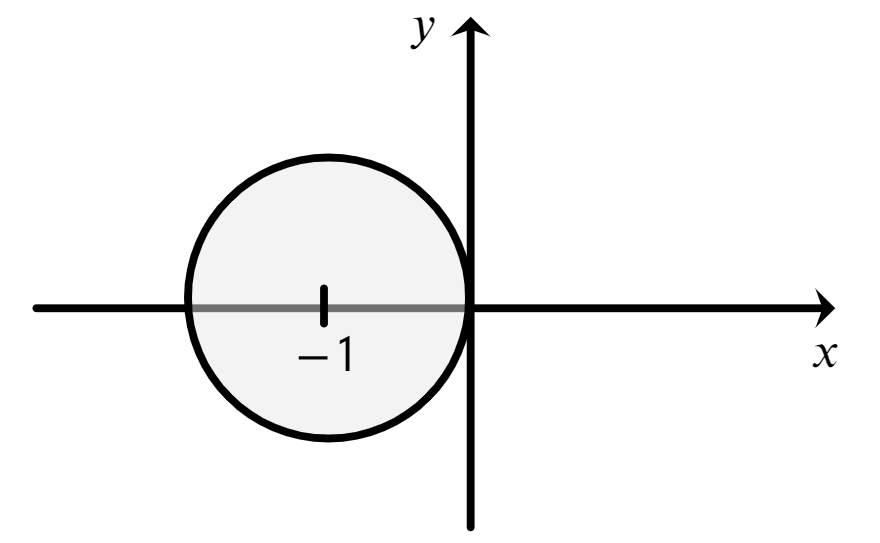
\includegraphics[scale=0.5]{img20}
	 	$$
	 	 Интервалом устойчивости является отрезок $[-2, 0]$. Легко видеть, что требования, чтобы все корни находились внутри круга единичного радиуса приводят к требованию, что если $\Re \lambda < 0$, то $ h \leq \dfrac{2}{|\lambda|}$. Также это требование можно считать \textbf{условием устойчивости явного метода Эйлера}.
	 	 \item \textbf{Неявный метод Эйлера.}\\\\
	 	 Если мы применим явный метод Эйлера для нашей модельной задачи, то получим другое характеристическое уравнение $$(1-z)y_{j+1} = y_j.$$
	 	 Отсюда $$y_{j+1} = \dfrac{1}{1-z}y_j.$$
	 	 Составим характеристическое уравнение и получим корень равный $$q = \dfrac{1}{1-z}.$$ Тогда условие устойчивости $$\left|\dfrac{1}{1-z}\right|\leq 1$$ а область устойчивости имеет вид
	 	 $$
			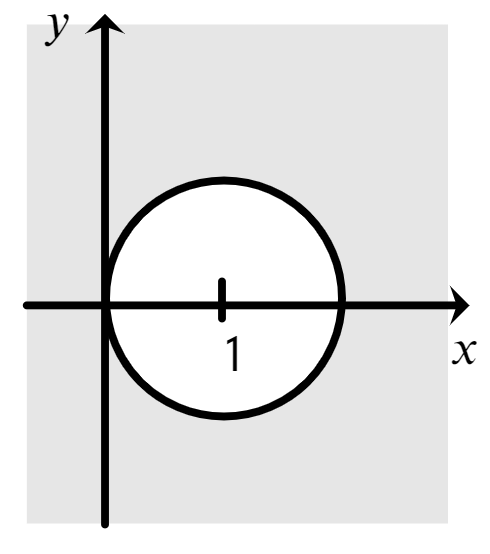
\includegraphics[scale=0.5]{img21}
	 	 $$
	 	 Интервалом устойчивости является вся действительная прямая за исключением отрезка $[0,2]$. Отсюда следует, что если $\Re \lambda < 0$ то $h$ может быть любым.
	 \end{enumerate}
	 $\bullet$ \textit{Численный метод будем называть \textbf{А-устойчивым (абсолютно устойчивым)}, если его область устойчивости содержит всю левую полуплоскость $\Re z < 0.$}\\\\
	 Другими словами, А-устойчивость подразумевает собой, что метод устойчивый $\forall h$.
	 Таким образом, неявный метод Эйлера является А-устойчивым, а явный метод Эйлера не является А-устойчивым.\\\\
	 В свое время было доказано, что не существует явных линейных А-устойчивых методов.\\\\
	 Запишем алгоритм, который применяется на практике для исследования устойчивости численных методов.
	 \begin{enumerate}
	 	\item применяя исследуемый метод к модельному уравнению (65), получаем разностное уравнение, которому удовлетворяет приближенное решение;
	 	\item записываем соответствующее характеристическое уравнение (аналог уравнения (66));
	 	\item находим корни этого уравнения $q_i$, $i=\overline{0,k}$;
	 	\item решая систему неравенств $|q_i| \leq 1$, $i=\overline{0,k}$, определяем область и интервал устойчивости метода.
	 \end{enumerate}
	 На практике чаще применяется способ определения области устойчивости, носящее название метода множества точек границы. Суть метода состоит в следующем. Если мы рассмотрим любую точку $z \in \Cm$, то эта точка будет принадлежать границе области устойчивости, если при данном значении $z$ выполняется равенство $$\underset{i}{\max}|q_i| = 1 = |q^*|,$$
	 причем обозначим $q^* = e^{i\varphi},\ \varphi \in [0, 2\pi].$ Решая записанное характеристическое уравнение относительно $z$, мы получаем множество точек, составляющих границу области устойчивости. Далее остается определить, например путем подстановки, по какую сторону границы находится сама область.\\\\
	 \textbf{Примеры.}
	 \begin{enumerate}
	 	\item \textbf{Метод последовательного повышения порядка точности второго порядка.}\\\\
	 	Для определенности возьмем формулу (29). Применительно к уравнению (65) этот метод имеет следующий вид $$y_{j+1} = \left(1+z + \dfrac {z^2}{2}\right)y_j.$$
	 	Тогда корень характеристического уравнения $$q = 1 + z + \dfrac{z^2}{2}.$$
	 	Поскольку найти область устойчивости уже сложнее, то в соответствии с описанным алгоритмом приравниваем $$q = 1 + z + \dfrac{z^2}{2} = e^{i\varphi}.$$
	 	Тогда получим $$z = z(\varphi) = - 1 \pm \sqrt {2e^{i\varphi}-1},\quad\varphi \in [0,2\pi].$$
	 	Кривая $z(\varphi)$ и есть граница области устойчивости, а сама область есть внутренняя часть ограниченная этой кривой. Интервал устойчивости равен в этом случае $[-2, 0]$.
	 	\item \textbf{Экстраполяционный метод Адамса второго порядка.}
	 	Применим формулу (54) к уравнению (65) и получим разностное уравнение $$y_{j+1}  - \left(1 + \dfrac{3z}{2}\right)y_j + \dfrac z 2 y_{j-1} = 0.$$
	 	Выписываем характеристическое уравнение $$q^2  - \left(1 + \dfrac{3z}{2}\right)q + \dfrac z 2  = 0.$$
	 	Подставляем $q = e^{i\varphi}$ и получаем функцию $$z = z(\varphi) = 2 \dfrac{e^{2i\varphi} - e^{i\varphi}}{3 e^{i\varphi} - 1}.$$
	 	Опять для разных $\varphi$ строим множество этих точек. \\\\
	 	При $\varphi = \pi$ мы получим точку $z(\pi) = -1$, а $z(0) = 0$. Получили интервал устойчивости $[-1, 0]$. А остальные точки позволят задать области устойчивости.  
	 \end{enumerate}
	 Вопрос об исследовании устойчивости одношаговых методов над полем действительных чисел упрощает процедуру исследования. В таком случае модельное уравнение (65) будет иметь вид $$u'(x) = \lambda u(x),\quad \lambda \in \Rm,\ \Re \lambda < 0.$$
	 Требованием устойчивости метода является неравенство $$|y_{j+1}|\leq |y_j|,\quad j = 0,1,\ldots.$$
	 Любой одношаговый метод может быть приведен к виду $$y_{j+1} = S(z) y_j,$$ где $S(z)$ --- множитель перехода от точки $x_j$ к точке $x_{j+1}$. Тогда метод является устойчивым, если выполняется неравенство $$|S(z)|\leq 1.$$ Значения $z$, при которых выполняется это неравенство, и будут являться интервалом устойчивости этого метода.
	 \\\\
	 \textbf{Примеры.}
	 \begin{enumerate}
	 	\item \textbf{Явный метод Эйлера.}\\\\
	 	Записываем метод в виде разностного уравнения $$y_{j+1} = (1+z) y_j.$$
	 	Тогда решаем неравенство $$S(z) = |1+z| \leq 1$$ над полем действительных чисел  и получаем $$-2 \leq z \leq 0.$$ Тогда $$0<h \leq -\dfrac 2 \lambda.$$
	 	\item \textbf{Неявный метод Эйлера.}\\\\
	 	В этом случае $$S(z) = \dfrac{1}{1-z}.$$
	 	Тогда $$\left|\dfrac{1}{1-z}\right|\leq 1,\quad \forall h > 0,$$
	 	а отсюда делаем вывод, что неявный метод Эйлера является А-устойчивым.
	 \end{enumerate}
	 \section{Методы решения краевых задач.}
	 \subsection{Понятия о многоточечных задачах.}
	 В многоточечных задачах дополнительное условие в дифференциальных уравнениях задаются в виде условий содержащих комбинации значений решения и его производных взятых в некоторых точках отрезка, где ищется решение.
	 \\\\
	 Будем считать, что на отрезке $[a,b]$ задано ОДУ $n$-ого порядка $$u^{(n)}(x) = f(x, u(x), u'(x), \ldots, u^{(n-1)}(x)),\ x \in [a,b].\eqno(1)$$
	 На отрезке $[a,b]$ выбраны $k$ различных точек $x_1, x_2,\ldots, x_k$ и в этих точках заданы условия $$v_j\big[u(x_1),\ldots, u^{(n-1)}(x_1),\ldots,u(x_k),\ldots, u^{(n-1)}(x_k)\big]=0,\ j=\overline{1,n}.\eqno(2)$$
	 $\bullet$ \textit{Уравнение $(1)$ и условия $(2)$ определяют \textbf{многоточечную ($k$-точечную) задачу}.}\\\\
	 В частном случае, когда $k=1$, а функции $v_j$ имеют тривиальный вид, мы получаем задачу Коши.\\\\
	 $\bullet$ \textit{Если $k=2$ и $x_1=a$, $x_2 = b$, то такая задача называется \textbf{краевой (граничной).}}\\\\
	 $\bullet$ \textit{Если исходное дифференциальное уравнение $(1)$ или хотя бы одно из дополнительных условий $(2)$ нелинейно, то имеем \textbf{нелинейную краевую задачу}. В противном случае задача называется \textbf{линейной}.}
	 \subsection{Метод редукции.}
	 Метод редукции предназначен для решения линейных краевых задач и основан на сведении линейной краевой задачи к решению задачи Коши.\\\\
	 Определим дифференциальное уравнение с помощью линейного дифференциального оператора
	 $$Lu \equiv u^{(n)}(x) + p_1(x) u^{(n-1)}(x) + \ldots + p_{n-1}(x)u'(x) + p_n(x)u(x) = f(x),\quad a < x < b.\eqno(3)$$
	 Граничные условия мы определим с помощью оператора $l$, в общем виде они будут иметь следующую структуру 
	 $$l_j(x) = \sum_{i=0}^{n-1}\left[\alpha_{ij} u^{(i)} (a) + \beta _{ij}u^{(i)}(b)\right] = \mu _j,\quad j = \overline{1,n},\eqno(4)$$
	 где заданы $\alpha_{ij}, \beta_{ij} = \operatorname{const}$, а количество условий должно совпадать с порядком уравнения. Тогда задача (1)-(2) превратилась в линейную краевую задачу (3)-(4).\\\\
	 Из теории дифференциальных уравнений известно, что общее решение задачи (3)-(4) представимо в виде линейной комбинации $$u(x) = u_0(x) + \sum_{i=1}^{n}C_iu_i(x),\eqno(5)$$
	 где $u_0(x)$ --- это некоторое частное решение неоднородного уравнения (3), а $u_i(x)$ --- решения соответствующего однородного уравнения, причем $u_i(x)$ образую линейную независимую систему. В формуле (5) $C_i$ --- это произвольные постоянные, конкретные значения которых определяются условием (4), а значит могут быть найдены из СЛАУ $n$-ого порядка вида 
	 $$
	 	l_j(u_0) + \sum_{i=1}^{n}C_i l_j(u_i) = \mu _j,\quad j = \overline{1,n}. \eqno (6)
	 $$
	 Если определитель матрицы системы (6) отличен от нуля, то будем иметь единственное решение. В противном случае либо бесконечное множество, либо задача не будет иметь решений, а значит задача будет являться некорректно поставленной.
	 \\\\
	 Таким образом, вопрос решения краевой задачи (3)-(4) сводится к тому, чтобы найти функции $u_0(x), u_1(x),\ldots, u_n(x)$. \\\\
	 При сделанных предположениях сведем задачу (3)-(4) к задачам Коши.\\\\
	 Функцию $u_0(x)$ будем определять из следующей задачи Коши
	 $$\begin{cases}
	 	L u_0(x) = f(x),\quad a<x< b,\\
	 	u_0(a) = 0,\\
	 	\dotfill\\
	 	u_0^{(n-1)}(a) = 0.
	 \end{cases}\eqno(7)$$
	 Функции $u_i(x)$ будем находить из следующей задачи Коши
	 $$
	 \begin{cases}
	 	L u_i(x) = 0,\\
	 	u_i^{(j)}(a)  = \delta_i^{j+1},\quad j = \overline{0,n-1}
	 \end{cases}\eqno(8)
	 $$
	 Такой выбор начальных условий обеспечивает линейную независимость функций $u_i(x)$.\\\\
	 Таким образом, решение краевой задачи (3)-(4) свелось к решению $(n+1)$ задач Коши. После этого из системы уравнений (6) мы найдем коэффициенты $C_i$. Тогда решение исходной задачи может быть представлено в виде (5).\\\\
	 Легко видеть, что решение, которое мы найдем, будет удовлетворять задаче (3)-(4). Мы также предполагаем, что задачи (7)-(8) решаются численно, а тогда возникает вопрос, как использовать полученные приближенные решения для того, чтобы решить краевую задачу.\\\\
	 \textbf{Замечания.}
	 \begin{enumerate}
	 	\item Метод редукции применим и для задач с нелинейными краевыми условиями. При этом для определения $C_i$ вместо СЛАУ необходимо решить соответствующую СНУ.
	 	\item Задачи Коши (7)-(8) могут быть решены с использованием рассматриваемых нами в параграфе 2 методов.
	 \end{enumerate}
	 \textbf{Пример.}
	 Алгоритм метода редукции запишем в случае $n=2$, причем для решения соответствующих задач Коши будем использовать метод Рунге-Кутты второго порядка. Тогда задачу (3)-(4) можем записать в виде 
	 $$Lu \equiv u''(x) + p_1(x)u'(x) + p_2(x)u(x) = f(x)$$
	 $$\begin{cases}
	 	\alpha_0 u(a) + \alpha_1 u'(a) = \mu_1,\\
	 	\beta_0 u(b) + \beta_1 b'(b) = \mu_2.
	 \end{cases}$$
	 Вместо (5) у нас будет $$u(x) = u_0(x) + C_1u_1(x) + C_2u_2(x).$$
	 Мы должны будем решить 3 задачи Коши. Вместо (7)-(8) у нас получится
	 $$\begin{cases}
	 	Lu_0(x) = f(x),\\
	 	u_0(a) = 0,\\
	 	u_0'(a) = 0.
	 \end{cases}\eqno (\rm{I})$$
	 $$\begin{cases}
	 	Lu_1(x) = f(x),\\
	 	u_1(a) = 1,\\
	 	u_1'(a) = 0.
	 \end{cases}\eqno (\rm{II})$$
	 $$\begin{cases}
	 	Lu_2(x) = f(x),\\
	 	u_2(a) = 0,\\
	 	u_2'(a) = 1.
	 \end{cases}\eqno (\rm{III})$$
	 Для решения задачи Коши мы будем применять численный метод, а значит мы будем находить решение в точках $[a,b]$. Для простоты предполагаем, что сетка равномерная.\\\\
	 Чтобы применить метод Рунге-Кутты, нам нужно свести уравнение 2-ого порядка к системе уравнений первого порядка с помощью замены
	 $$\begin{cases}
	 	u'_0(x) = v_0(x),\\
	 	v_0'(x) = -p_1(x)v_0(x) - p_2(x) u_0(x) + f(x),\\
	 	u_0(a) = 0,\\
	 	v_0(a) = 0.
	 \end{cases}\eqno (\rm{I'})$$
	 $$\begin{cases}
	 	u'_1(x) = v_1(x),\\
	 	v_1'(x) = -p_1(x)v_1(x) - p_2(x) u_1(x),\\
	 	u_1(a) = 1,\\
	 	v_1(a) = 0.
	 \end{cases}\eqno (\rm{II'})$$
	 $$\begin{cases}
	 	u'_2(x) = v_2(x),\\
	 	v_2'(x) = -p_1(x)v_2(x) - p_2(x) u_2(x),\\
	 	u_2(a) = 0,\\
	 	v_2(a) = 1.
	 \end{cases}\eqno (\rm{III'})$$
	 Запишем формулы метода Рунге-Кутта применительно к векторному уравнению
	 $$
	 \begin{cases}
	 	\overline u' = \overline f(x, \overline u(x)),\\
	 	\overline u (a) = \overline u_0,
	 \end{cases}\quad 
	 \overline u = \begin{pmatrix}
	 u_1(x) \\ u_2(x)
	 \end{pmatrix},\quad
	 \overline f = \begin{pmatrix}
	 	f_1(x, u_1(x), u_2(x)),\\
	 	f_2(x, u_1(x), u_2(x)),
	 \end{pmatrix}\quad
	 \overline u_0 = \begin{pmatrix}
	 	u_{01} \\ u_{02}
	 \end{pmatrix}.
	 $$
	 В итоге получим систему 
	 $$
	 \begin{cases}
	 	u_1'(x) = f_1(x, u_1, u_2),\\
	 	u_2'(x) = f_2(x, u_1, u_2),\\
	 	u_1(a) = u_{01},\\
	 	u_2(a) = u_{02}.
	 \end{cases}
	 $$
	 Метод Рунге-Кутта 2-ого порядка по формуле (40) из параграфа 2 имеет вид 
	 $$\overline y_{j+1} = \overline y_j + h\overline f\left(x_j + \dfrac 12 h , \overline y_j + \dfrac 12 h \overline f_j\right),\quad \overline y_j = \begin{pmatrix}
	 	y_1(x_j) = y_{1,j}\\
	 	y_2(x_j) = y_{2,j}
	 \end{pmatrix}$$
	 Распишем эту формулу по координатам
	 $$\begin{cases}
	 	y_{1, j+1} = y_{1,j} + hf_1\left(x_j + \dfrac 12 h, y_{1,j} + \dfrac 12 hf_1(x_j, y_{1,j}, y_{2,j}), y_{2,j} + \dfrac12 h f_2(x_j, y_{1,j}, y_{2,j})\right),\\
	 	y_{2, j+1} = y_{2,j} + hf_2\left(x_j + \dfrac 12 h, y_{1,j} + \dfrac 12 hf_1(x_j, y_{1,j}, y_{2,j}), y_{2,j} + \dfrac12 h f_2(x_j, y_{1,j}, y_{2,j})\right)
	 \end{cases}$$
	 Здесь легко видеть, что вместо одного массива будет два массива и для $j = \overline{0, N-1}$ можно организовать рекуррентные формулы для вычисления всех значений $y$, причем
	 $$y_{1,0} = u_{01}, y_{2,0} = u_{02}.$$
	 Таким образом, решение задачи $(\rm{I}')$, то есть функции $u_0(x)$, $v_0(x)$, будем искать в точках отрезк $$x_j = a+jh,\ h = \dfrac{b-a}{N},\ j = \overline{0,N}.$$
	 Обозначим 
	 $$u_0(x) \approx y_0(x_j) = y_{0,j},$$
	 $$v_0(x_j) \approx z_0(x_j) = z_{0,j}.$$
	 Нужно, применяя формулы, найти значения во всех узлах $x_j$:
	 $$\begin{cases}
	 	y_{0, j+1} = y_{0,j} + h\left(z_{0,j} + \dfrac12 h(-p_{1,j} z_{0,j} - p_{2,j}y_{0,j} + f_j)\right),\\
	 	z_{0,j+1} = z_{0,j} + h\left( -p_{1, j+\frac12}(z_{0,j} + \dfrac 12 h (-p_{1,j} z_{0,j} - p_{2,j} y_{0,j} + f_j) - p_{2, j+\frac12} (y_{0,j} + \dfrac12 hz_{0,j}) + f_{j+\frac12})\right),\\
	 	y_{0,0} = 0,\\
	 	z_{0,0} = 0,\quad j = \overline{0,N-1}.
	 \end{cases}$$
	 Аналогично решив задачи $(\rm{II}')$ и $(\rm{III}')$ мы получим приближенные значения функций $y_{1,j}, z_{1,j}$, $y_{2,j}, z_{2,j}$, $j = \overline{0,N-1}$.\\\\
	 Осталось определить константы $C_1, C_2$. Для это подставляем $u(x)$ в краевые условия исходной задачи и получим для определения $C_1$ и $C_2$ СЛАУ второго порядка
	 $$
	 \begin{cases}
	 	\alpha_0 C_1 + \alpha_1 C_2 = \mu _1,\\
	 	\beta_0 (y_{0,N} + C_1y_{1, N} + C_2 y_{2,N}) + \beta_1 (z_{0,N} + C_1z_{1, N} + C_2 z_{2,N}) = \mu_2.
	 \end{cases}
	 $$
	 После того, как мы найдем значения $C_1$, $C_2$, мы можем записать решения задачи в узлах $$y(x_j) = y_0(x_j) + C_1y_1(x_j) + C_2 y_2(x_j),\quad j=\overline{0, N}.$$
	 \subsection{Метод стрельбы.}
	 Данный метод как и метод редукции основан на сведении решения краевой задачи к решению задачи Коши. При этом он применим и для решения нелинейных задач, а в случае линейных краевых задач позволяет уменьшить объем вычислений.
	 \subsubsection{Метод стрельбы для линейных краевых задач.}
	 Рассмотрим идею метода на примере задачи для уравнения второго порядка
	 $$\begin{cases}
	 L u(x)\equiv u''(x) + p_1(x)\cdot u'(x) + p_2(x)\cdot u(x) = f(x), \ a<x<b,\\
	 u(a) = \mu _1,\\
	 u(b) = \mu_2.
	 \end{cases}\eqno(9)$$
	Пусть $u_0(x)$ --- это частное решение задачи (9), но не с произвольными начальными условиями, а зададим такие начальные условия, чтобы оно удовлетворяло левому граничному условию в точке $x=a$. Тогда
	$$\begin{cases}
		Lu_0(x) = f(x), \\ u_0(a) = \mu_1,\\ u'_0(a) = \eta_0.\\ 
	\end{cases}\eqno(10)$$
	В уравнении (10) $\eta_0$ --- произвольная постоянная.
	Рассмотрим также частное решение $u_1(x)$ однородного уравнения
	$$\begin{cases}
		Lu_1(x) = 0, \\ u_1(a) = 0, \\ u'_1(a) = \eta_1.
	\end{cases}\eqno(11)$$
	Если мы составим линейную комбинацию $$u(x) = u_0(x) + Cu_1(x),\eqno(12)$$
	то данная функция заведомо удовлетворяет исходному ДУ и его граничному условию при любом значении произвольной постоянной C.
	$$u_0(b) + C u_1(b) = \mu_2,$$
	тогда $$C = \dfrac{\mu_2 - u_0(b)}{u_1(b)},\ u_1(b)\ne 0.\eqno(13)$$
	Изложим метод стрельбы в общем случае для системы ЛОДУ-1 
	$$\begin{cases}
		u'(x) = A(x)\cdot u(x) + f(x),\\
		Bu(a) = c,\\
		Du(b) = d;
	\end{cases}\eqno(14)$$
	где $u(x), f(x), c, d$ --- это векторы размерностей $n, n, n-r, r$ соответственно, $A(x), B, D$ --- матрицы размерностей $n\times n, (n-r)\times n, r\times n$. Предположим, что $$\rank B = n-r, \ \rank D = r.$$
	Для системы (14) рассмотрим метод стрельбы. СЛАУ $$Bu = c\eqno(15)$$ задает граничное условие на левом конце отрезка $[a,b]$. Так как $\rank B = n-r$, то общее решение этой системы может быть записано в виде $$u = u_0 + \sum_{i=1}^{r}c_i u_i.$$
	где $u_0$ --- это произвольное решение неоднородной системы (15), а $u_1,\ldots, u_r$ --- это произвольная система из $r$ линейно независимых решений соответствующей однородной системы $$Bu = 0.$$
	Пусть мы определили функции $u_0, u_1,\ldots, u_r$. Тогда мы можем рассмотреть задачу $$\begin{cases}
		u_0'(x) = A(x)\cdot u_0(x) + f(x),\\
		u_0(a) = u_0.
	\end{cases}\eqno(16)$$
	Остальные функции $u_1,\ldots, u_r$ мы можем найти исходя из решения соответствующей однородной системы:
	$$\begin{cases}
		u_j'(x) = A(x)\cdot u_j(x),\\
		u_j(a) = u_j;
	\end{cases}j=\overline {1,r}.\eqno(17)$$
	Предположим, что мы решили задачи (16) и (17). Тогда мы можем составить функцию 
	$$u(x) = u_0(x) + \sum_{j=1}^{r}c_j u_j(x).\eqno(18)$$
	Видно, что для любых $c_j$ функции $u_j(x)$ удовлетворяет левому граничному условию задачи (14). Постоянные $c_j$ определяются из следующего 
	$$D\left(u_0(b) + \sum_{j=1}^{r}c_ju_j(b)\right) = d.\eqno(19)$$
	Уравнение (19) представляет собой СЛАУ размерности $r\times r$. Матрица этой системы невырождена, поэтому система имеет единственное решение. \\\\
	Окончательно сформулируем алгоритм метода стрельбы решения задачи (14). \begin{enumerate}
		\item Находим частное решение $u_0$ неоднородной системы (15) и $r$ линейно независимых частных решений соответствующей однородной системы $u_1,\ldots, u_r$.
		\item Решаем задачу Коши (16)-(17) начальными условиями которых являются найденные на первом этапе решения значения функции $u_0, u_1,\ldots, u_r$.
		\item Составляем и решаем систему (19) и находим $c_j$, $j = \overline{1,r}$
		\item По формуле (18) определяем решение исходной краевой задачи (14).
	\end{enumerate} 
	Важно, чтобы выполнялось $r+1 < n$. В зависимости от размерности матриц $B$ и $D$ подбирается общее количество решаемых задач Коши, которое будет минимальным. Например, если $n-r < r$, то начальные условия следует подбирать не на левом конце, а на правом конце, то есть решая систему $Du = d$. Тогда общее количество задач Коши будет $(n-r+1)$.
	\subsubsection{Метод стрельбы для нелинейных задач.}
	Рассмотрим алгоритм метода стрельбы в случае, когда исходное уравнение нелинейно, а граничные условия первого рода
	$$\begin{cases}
		u''(x) = f(x, u(x), u'(x)),\ a<x<b,\\
		u(a) = \mu_1,\\
		u(b) = \mu_2.
	\end{cases}\eqno(20)$$
	В данном случае метод стрельбы превращается в сведение краевой задачи к сведению задач Коши для того же уравнения, но с различными начальными условиями
	$$u(a) = \mu_1,\ u'(a) = \eta,\eqno(21)$$
	где $\eta$ --- произвольный параметр.\\\\
	Предположим, что $\eta = \tg \alpha$, где $\alpha$ --- угол наклона касательной к интегральной кривой в точке $x=a$.
	$$
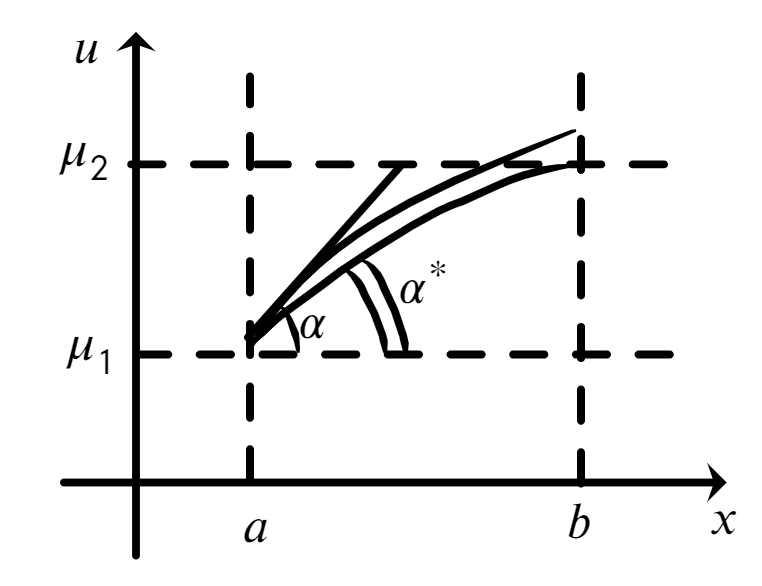
\includegraphics[scale=0.5]{img22}
	$$
	Считая решение задачи зависящим от параметра $\eta$, будем искать такую интегральную кривую $u(x,\eta^*)$, которая выходит из точки $(a, \mu_1)$ и попадает в точку $(b, \mu_2)$.
	Для определения $\eta$ можно записать простое уравнение относительно $\eta$: $$F(\eta) = u(b, \eta) - \mu_2 = 0.\eqno(22)$$
	Хотя уравнение (22) нельзя представить в виде некоторого аналитического выражения, но для его решения могут быть использованы методы рассматриваемых ранее нелинейных уравнений.\\\\
	Запишем алгоритм метода стрельбы с реализацией по методу половинного деления отрезка.
	Рассматриваем начальную задачу
	$$\begin{cases}
		u''(x) = f(x, u(x), u'(x)),\ a<x<b,\\
		u(a) = \mu_1,\\
		u'(a) = \eta.
	\end{cases}\eqno(20)$$
	\begin{enumerate}
		\item При различных значениях $\eta$ находим отрезок $[\eta_0, \eta_1]$, на котором функция $F(\eta)$ меняет знак.
		\item Берем $\eta_2 = \dfrac{\eta_0 + \eta_1}{2}$ и снова решаем задачу Коши (23).
		\item Сужаем отрезок до тех пор, пока $|\eta_{k+1} - \eta_k|\leq \epsilon$. Тогда решение найденное при последнем значении $\eta$ и является приближенным значением исходной задачи (20) $u(x, \eta_{k+1})\approx u(x)$.
	\end{enumerate}
	Можно на этапе 2 применять методы с более высокой скоростью сходимости. На практике часто берут метод секущих. По методу секущих каждое последующее приближение будет вычисляться по формуле
	$$\eta_{k+1} = \eta_k - \dfrac{(\eta_k - \eta_{k-1}) F(\eta_k)}{F(\eta_k)-F(\eta_{k-1})},\ k=1,2,\ldots.\eqno(24)$$
	Скорость процесса (24) зависит от выбора $\eta_0$ и $\eta_1$.\\\\
	В случае условия на левой границе для производной $$u'(a) = \mu_1,\ u(b) = \mu _2$$ пристрелку нужно проводить не по углу наклона интегральной кривой, а по ее расположению в начальной точке.
	\\\\
	Рассмотрим случай двух уравнений с двумя неизвестными и с нелинейными краевыми условиями. Пусть дана задача $$\begin{cases}
		u'(x) = f(x, u(x), v(x)),\ a<x<b,\\
		v'(x) = g(x, u(x), v(x)),\ a<x<b,\\
		\varphi(u(a), v(a)) = 0,\\
		\psi (u(b), v(b)) = 0.
	\end{cases}\eqno(25)$$
	Сразу сформулируем алгоритм.
	\begin{enumerate}
		\item Выберем произвольное значение $u(a) = \eta$. Из левого граничного условия выразим $v(a) = \xi(\eta)$, где $\xi$ --- известная функция
		При этих начальных условиях будем решать задачу Коши вида
		$$\begin{cases}
			u'(x) = f(x, u(x), v(x)),\ a<x<b,\\
			v'(x) = g(x, u(x), v(x)),\ a<x<b,\\
			u(a) = \eta,\\
			v(a) = \xi(\eta).
		\end{cases}\eqno(26)$$
		\item Вычисляем значение $\eta_0, \eta_1,\ldots,\eta_k,\ldots$ по любому методу (половинного деления, секущих и так далее) из уравнения $$\psi(\eta) = \psi(u(b,\eta), v(b,\eta)) = 0.$$
		\item Если выполнено условие остановки $|\eta_{k+1} - \eta_k|< \epsilon$, то решениями будут являться функции $u(x, \eta_{k+1})$ и $v(x, \eta_{k+1})$.
	\end{enumerate}
	Мы можем обобщить этот метод до большего числа уравнений и неизвестных, но тогда выполнение правого краевого условия становится сложнее обеспечить с точки зрения реализации методов решения нелинейных уравнений в многомерном случае.
	\subsection{Метод Ритца.}
	Метод Ритца является одним из известных вариационных методов решения задач математической физики.
	\\\\
	Пусть $H$ --- некоторое вещественное гильбертово пространство со скалярным произведением $(\cdot, \cdot)$ и нормой, которая определяется через скалярное произведение $\Norm{\cdot} = \sqrt{(\cdot, \cdot)}$. Обозначим через $A$ линейный оператор, определенный на множестве $H_A$, то есть $$A:H_A \to H.$$ Тогда мы можем рассматривать операторное уравнение $$Au = f,\eqno(28)$$ где $f$ --- заданный элемент в пространстве $H$, а $u\in H_A$  --- искомый элемент. Можно доказать, что если $A = A^* > 0,$ то уравнение (28) не может иметь более одного решения, то есть если его решение существует, то оно будет единственно. Задача нахождения решения уравнения (28) равносильна нахождению такого элемента $u$, доставляющего минимум функционала $$\mathcal J(u) = (Au, u) - 2(f,u).\eqno(29)$$
	Метод Ритца состоит в следующем. Для решения задачи минимизации функционала (29), то есть нахождения такого элемента $u^* \in H_A$, что $$\mathcal J(u^*) = \underset{u \in H_A}{\min}\mathcal J(u).$$
	В пространстве $H_A$ рассмотрим последовательность конечномерных пространств $\{H_n\}$, $n=1,2,\ldots$ таких, что всякий элемент $u\in H_A$может быть с любой степенью точности приближен его элементами (свойство полноты). 
	Таким образом, требуется построить последовательность элементов $\{u_n\}$, $u_n \in H_n$, доставляющую минимум функционала $\mathcal J (u_n)$ в пространстве $H_n$ $$\mathcal J (u_n) = m_n \xrightarrow[n\to\infty]{} m = \mathcal J (u).$$
	Если при этом $u_n \xrightarrow[n\to\infty]{}u^*$, то любой элемент $u_n$ можно брать в качестве приближенного значения к $u^*$.\\\\
	Предположим, что в пространстве $H_n$ известен базис $\varphi_i$. Тогда построение минимизирующей последовательности эквивалентно нахождению коэффициентов $a_i$ разложения $$u_n = \sum_{i=1}^n a_i \varphi_i\eqno(30)$$ из условия минимума функционала $\mathcal J(u_n)$. Подставим (30) в (29), тогда получим $$\mathcal J(u_n) = (Au_n, u_n)-2(f, u_n)=\sum_{i=1}^n \sum_{j=1}^n a_i a_j (A\varphi_j, \varphi_i) - 2\sum_{i=1}^n q_i(f_i,\varphi_i)=\Phi(a_1,\ldots, a_n).$$
	Таким образом, минимизация функции от $n$ переменных --- это более простая задача. Минимум функции $\Phi$ достигается, если $$\dfrac{\partial \Phi}{\partial a_i}=0, \ \dfrac{\partial^2 \Phi}{\partial a_i^2} >0,\ i = \overline{1,n}$$
	Причем единственность функционала следует из того, что $$\dfrac{\partial^2 \Phi}{\partial a_i^2} >0.$$
	И $$\dfrac{\partial \Phi}{\partial a_i} = 2\sum_{j=1}^n a_j(A\varphi_j, \varphi_i)- 2(f_i, \varphi_i)=0,\ i=\overline{1,n}.$$
	Тогда получаем СЛАУ $$\sum_{j=1}^{n}c_{ij}a_j = d_i,\ i=\overline{1,n},$$ где коэффициенты матрицы $c_{ij} = (A\varphi_j ,\varphi_i)$, $d_i = (f, \varphi_i)$, $i,j = \overline{1,n}$. Решив систему (31), приближенное решение исходной задачи находим по формуле (30).\\\\
	Рассмотрим метод Ритца применительно к краевой задаче следующего вида с однородными граничными условиями первого рода
	$$\begin{cases}
		Au\equiv -(k(x) u'(x))' + q(x)u(x) = -f(x),\ a<x<b,\\
	u(a)=u(b) = 0
	\end{cases}\eqno(32)$$
	В задаче (32) $k(x)\geq k_0 > 0$, $k(x) \in C^1[a,b]$, $q(x)\geq 0$, $q(x) \in C[a,b]$, $f(x)\in C[a,b]$. Эта задача описывает стационарное одномерное уравнение теплопроводности, где $u(x)$ --- функция, описывающая температуру стержня нулевого сечения, $k$ --- коэффициент теплопроводности, $q(x)$ и $f(x)$ отвечают за внутренние и внешние источники стока тепла соответственно. Более того именно для такого оператора можно доказать все необходимые теоремы для использования вариационного подхода. \\\\
	Оператор $A$ на множестве $$H_A=\{ u(x)\in W_2^1 | u(a)=u(b) = 0\}$$ является самосопряженным. Действительно 
	$$\forall u, v \in H_A\quad (Au, uv) = \int\limits_a^b ((-k(x)u'(x))' + q(x)u(x))v(x)dx = -ku' v\Big|_a^b + \int\limits_a^b (ku'v' + quv)dx = (Av, u),$$
	$$(Au, u) = \int\limits_a^b (-(ku')'+qu))udx > 0,$$
	то есть выполняется условие, необходимое для того, чтоб применить метод Ритца. \\\\
	Применяя метод Ритца, формула (29) превратится в следующий функционал $$\mathcal J(u) = \int\limits_a^b (k(u')^2 + qu^2 + 2fu)dx.\eqno(33)$$
	Мы должны построить минимизирующую последовательность. Для этого выберем последовательность базисных функций $\{\varphi_i(x)\}$ такую, что \begin{enumerate}
		\item $\varphi_i(x) \in C^1 [a,b],\ i=1,2,\ldots$, причем $\varphi_i(a) = \varphi_i(b) = 0$;
		\item $\forall h$ $\varphi_1,\ldots, \varphi_n$ линейно независимые;
		\item образованное по множеству функций $\{\varphi_i\}$ семейство функций $\{u_n\}$, где $u_n$ определяется по формуле (30), в пространстве $C^1[a,b]$ обладает свойством полноты.
	\end{enumerate}
	Таким образом, мы можем построить $u_n$, а для каждого $n$ можем найти свой набор коэффициентов $a_i$. $$\sum_{j=i}^{n}c_{ij}a_j = d_i, i = \overline {1,n},\eqno(34)$$
	$$c_{ij} = \int\limits_a^b (k(x)\varphi_j ' \varphi _i ' + q(x) \varphi_j \varphi_i)dx,$$
	$$d_i = -\int\limits_a^b f(x)\varphi_i(x)dx.$$
	СЛАУ (34) разрешима и имеет единственное решение для любого $n$. В качестве $\varphi_i(x)$ можно выбирать следующие:
	\begin{enumerate}
		\item $\varphi_i(x) = (x-a)^i(x-b)$, $\varphi_i(x) = (x-a)(x-b)^i$, $i=1,2,\ldots$;
		\item $\varphi_i(x) = \sin i\pi \dfrac{x-a}{b-a}$, $i=1,2,\ldots$.
	\end{enumerate}
	Подытоживая, запишем алгоритм метода Ритца:
	\begin{enumerate}
		\item выбираем систему базисных функций $\varphi_i(x)$;
		\item составляем систему (34) для заданного значения $n$, решаем ее и получаем значения $a_i$;
		\item по $a_i$ строим $u_n(x)$ по формуле (30).
	\end{enumerate}
	Функция $u_n(x)$ и будет являться приближенным решением к решению нашей задачи.
	\textbf{Замечания.}
	\begin{enumerate}
		\item Если поставлена третья краевая задача с условиями третьего рода $$\alpha_0 u(a) + \alpha_1 u'(a) = \mu_1,$$ $$\beta_0 u(a)+\beta_1 u'(b)=\mu _2,$$
		то можно сформировать $$u_n(x) = \varphi_0 + \sum_{i=1}^n a_i\varphi_i.\eqno(35)$$ 
		$\varphi_0$ --- это функция, удовлетворяющая граничным условиям, а функции $\varphi_i$ и $\varphi_i'$ обращаются в ноль на концах отрезка. При сделанных предположениях функция $\varphi_n(x)$ также будет удовлетворять поставленным краевым условиям. При этом $a_i$ можно находить из системы (34) с немного измененной правой частью:
		$$d_i = -\int_a^b (f\varphi_i + k(x)\varphi_0' \varphi_i' + q(x)\varphi_0 \varphi_i)dx.\eqno(36)$$ 
		В данном случае можно выбрать $$\varphi_0(x) = C_0x + C_1,$$ где $C_0$, $C_1$ --- это постоянные, которые принадлежат определению из системы уравнений $$\begin{cases}
			\alpha_0 (C_0a + C_1) + \alpha_1 C_0 = \mu _1,\\
			\beta_0(C_0 b + C_1) + \beta_1 C_1 = \mu _2;
		\end{cases}$$ а $$\varphi_i(x) = (x-a)^{i+1}(x-b)^2, \ i= \overline{1,n}.$$
		\item 
	\end{enumerate}
	\subsection{Метод Галеркина.}
	Основным недостатком метода Ритца является то, что он применим только для уравнений с самосопряженным положительно определенным оператором. Идея метода Ритца была доказана для случая несамосопряженного оператора. Подход остается тот же: мы будем искать приближенное решнеие по прежнему в виде (30), но коэффициенты будем определять из условия невязки в системе функций $\varphi_i$, а именно $$(Au_n - f, \varphi_i) = 0,\ i=1,2,\ldots,n.\eqno(37)$$
	Можно показать, что из условий (37) для вычисления коэффициентов $a_i$ получим систему (34), но на оператор $A$ не накладывается условий самосопряженности и положительности. 
	Например, $$\begin{cases}
		u''(x) + p(x) u'(x) + q(x)u(x) = f(x), \ a< x < b,\\
		u(a) = 0,\\
		u(b) = 0.
	\end{cases}\eqno(38)$$
	Проделывая аналогичные методу Ритца действия, получим систему (34), в которой $$c_{ij} = \int\limits_a^b (\varphi_j'' + p\varphi_j' + q\varphi_j)dx,\ d_i = \int\limits_a^b f(x)\varphi_i(x)dx.$$
	Метод Галеркина является обобщением метода Ритца и в частном случае с самосопряженным положительным оператором он превращается в метод Ритца.\\\\
	Метод Галеркина в свою очередь является частным случаем метода моментов. Метод моментов основан на том, что мы ищем элемент $u_n$, ортогональный некоторой системе функций $$(Au_n-f, \psi_i) = 0,\ \varphi_i \ne \psi_i.\eqno(40)$$
	
	\end{document}
	


	